%%% On-going present
%%
%% Beginning of file 'sample.tex'
%%
%% Modified 2005 December 5
%%
%% This is a sample manuscript marked up using the
%% AASTeX v5.x LaTeX 2e macros.

%% The first piece of markup in an AASTeX v5.x document
%% is the \documentclass command. LaTeX will ignore
%% any data that comes before this command.

%% The command below calls the preprint style
%% which will produce a one-column, single-spaced document.
%% Examples of commands for other substyles follow. Use
%% whichever is most appropriate for your purposes.
%%
%%\documentclass[12pt,preprint]{aastex}

%% manuscript produces a one-column, double-spaced document:

%%\documentclass[manuscript]{aastex}

%% preprint2 produces a double-column, single-spaced document:

 %\documentclass[preprint2]{aastex}
%\documentclass[preprint2]{aastex}
%\documentclass[manuscript]{aastex}
\documentclass[iop]{emulateapj}
\usepackage{color}
\renewcommand{\baselinestretch}{0.95}
%% Sometimes a paper's abstract is too long to fit on the
%% title page in preprint2 mode. When that is the case,
%% use the longabstract style option.

%% \documentclass[preprint2,longabstract]{aastex}

%% If you want to create your own macros, you can do so
%% using \newcommand. Your macros should appear before
%% the \begin{document} command.
%%
%% If you are submitting to a journal that translates manuscripts
%% into SGML, you need to follow certain guidelines when preparing
%% your macros. See the AASTeX v5.x Author Guide
%% for information.

\usepackage{enumitem} 

\newcommand{\hMsun}{{\ifmmode{h^{-1}{\rm
        {M_{\odot}}}}\else{$h^{-1}{\rm{M_{\odot}}}$~}\fi}} 
\newcommand{\hMpc}{{\ifmmode{h^{-1}{\rm Mpc}}\else{$h^{-1}$Mpc }\fi}}
\def\be{\begin{equation}}
\def\ee{\end{equation}}
\def\ba{\begin{eqnarray}}
\def\ea{\end{eqnarray}}

\newcommand{\scr}{\textcolor{red}}


%% You can insert a short comment on the title page using the command below.

%\slugcomment{Not to appear in Nonlearned J., 45.}

%% If you wish, you may supply running head information, although
%% this information may be modified by the editorial offices.
%% The left head contains a list of authors,
%% usually a maximum of three (otherwise use et al.).  The right
%% head is a modified title of up to roughly 44 characters.
%% Running heads will not print in the manuscript style.

%\title[]
%{}

\shorttitle{Reshift Dependent Volume effect}
\shortauthors{X.-D. Li, C. Park, C.G. Sabiu, H. Park, C. Cheng, J. Kim, S.E. Hong}

%% This is the end of the preamble.  Indicate the beginning of the
%% paper itself with \begin{document}.

\begin{document}

%% LaTeX will automatically break titles if they run longer than
%% one line. However, you may use \\ to force a line break if
%% you desire.

\title{Cosmological constraints from the redshift dependence of the volume effect using the galaxy 2-point correlation function across the line-of-sight}


%\author{Xiao-Dong~Li\altaffilmark{1}, Changbom~Park\altaffilmark{1}, J.~E.~Forero-Romero\altaffilmangulatark{2} and Juhan Kim%\altaffilmark{3}}
%\affil{\altaffilmark{1}School of Physics, Korea Institute for Advanced Study, Heogiro 85, Seoul 130-722, Korea }
%\affil{\altaffilmark{2}Departamento de F\'{i}sica, Universidad de los Andes, Cra. 1 No. 18A-10, Edificio Ip, Bogot\'a, %Colombia}
%\affil{\altaffilmark{3}Center for Advanced Computation, Korea Institute for Advanced Study, 85 Hoegi-ro, Dongdaemun-%gu, Seoul 130-722, Korea }
%\affil{\it (xiaodongli@kias.re.kr, cbp@kias.re.kr, je.forero@uniandes.edu.co, kjhan@kias.re.kr)}

%\author[Xiao-Dong~Li, Changbom~Park, Cristiano G. Sabiu, Juhan Kim and Sungwook E. Hong]
%{ Xiao-Dong Li$^{1,\dagger}$, Changbom Park$^{1}$, Cristiano G. Sabiu$^{2}$, Juhan Kim$^{3,1,\star}$, Sungwook E. Hong$^{1}$\\
%$^1$School of Physics, Korea Institute for Advanced Study, 85 Heogi-ro, Dongdaemun-gu, Seoul 130-722, Korea\\
%$^2$Korea Astronomy and Space Science Institute, 776, Daedeokdae-ro, Yuseong-gu, Daejeon, 305-348, Korea\\
%$^3$Center for Advanced Computation, Korea Institute for Advanced Study, 85 Hoegi-ro, Dongdaemun-gu, Seoul 130-722, Korea\\
%$^{\dagger}$xiaodongli@kias.re.kr\\
%$\star$Corresponding Author: ***@kasi.re.kr}

\author{Xiao-Dong Li, Changbom Park, }
\affil{School of Physics, Korea Institute for Advanced Study, 85 Heogiro, Dongdaemun-gu, Seoul 130-722, Korea}
\author{Cristiano G. Sabiu\altaffilmark{1}, Hyunbae Park, }
\affil{Korea Astronomy and Space Science Institute, Daejeon 305-348, Korea}
%\author{David H. Weinberg,}
%\affil{Department of Astronomy and CCAPP, The Ohio State University, 140 West 18th Avenue, Columbus, OH 43210, USA}
%\author{Donald P. Schneider,}
%\affil{Department of Astronomy and Astrophysics, The Pennsylvania State University, 
%University Park, PA 16802 }
%\affil{Institute for Gravitation and the Cosmos, The Pennsylvania State University, 
%University Park, PA 16802 }
\author{Cheng Cheng, }
\affil{Kavli Institute for Theoretical Physics China, Institute of Theoretical Physics, Chinese Academy of Sciences, Zhong Guan Cun Street 55\#, Beijing, 100190, P.R. China}
\affil{University of Chinese Academy of Sciences, P.R. China}
\author{Juhan Kim,}
\affil{Center for Advanced Computation, Korea Institute for Advanced Study, 85 Hoegi-ro, Dongdaemun-gu, Seoul 130-722, Korea}
\and
\author{Sungwook E. Hong}
\affil{School of Physics, Korea Institute for Advanced Study, 85 Heogiro, Dongdaemun-gu, Seoul 130-722, Korea}
\affil{Korea Astronomy and Space Science Institute, Daejeon 305-348, Korea}

%\altaffiltext{1}{xiaodongli@kias.re.kr}
%\altaffiltext{2}{cbp@kias.re.kr}
%\altaffiltext{3}{csabiu@kasi.re.kr}
%\altaffiltext{4}{\bf Hyunbae: your email}
\altaffiltext{1}{Corresponding Author: csabiu@kasi.re.kr}

% \email{xiaodongli@kias.re.kr}
% \email{cbp@kias.re.kr}
% \email{je.forero@uniandes.edu.co}



% \author{S. Djorgovski\altaffilmark{1,2,3} and Ivan R. King\altaffilmark{1}}
% \affil{Astronomy Department, University of California,
%     Berkeley, CA 94720}
%
% \author{C. D. Biemesderfer\altaffilmark{4,5}}
% \affil{National Optical Astronomy Observatories, Tucson, AZ 85719}
% \email{aastex-help@aas.org}
%
% \and
%
% \author{R. J. Hanisch\altaffilmark{5}}
% \affil{Space Telescope Science Institute, Baltimore, MD 21218}
%
% %% Notice that each of these authors has alternate affiliations, which
% %% are identified by the \altaffilmark after each name.  Specify alternate
% %% affiliation information with \altaffiltext, with one command per each
% %% affiliation.
%
% \altaffiltext{1}{Visiting Astronomer, Cerro Tololo Inter-American Observatory.
% CTIO is operated by AURA, Inc.\ under contract to the National Science
% Foundation.}
% \altaffiltext{2}{Society of Fellows, Harvard University.}
% \altaffiltext{3}{present address: Center for Astrophysics,
%     60 Garden Street, Cambridge, MA 02138}
% \altaffiltext{4}{Visiting Programmer, Space Telescope Science Institute}
% \altaffiltext{5}{Patron, Alonso's Bar and Grill}

%% Mark off your abstract in the ``abstract'' environment. In the manuscript
%% style, abstract will output a Received/Accepted line after the
%% title and affiliation information. No date will appear since the author
%% does not have this information. The dates will be filled in by the
%% editorial office after submission.

\begin{abstract}
We propose to use the redshift dependence of the galaxy 2-point correlation function across the line-of-sight (2pCF), $\xi(r_{\bot})$, to constrain cosmological parameters.
When an incorrect set of cosmological parameters is assumed for transforming galaxy redshifts to comoving distances, 
it produces {\it redshift-dependent mis-scaling} in the galaxy distribution.
As a result, we observe a redshift-dependent rescaling in the measured $\xi(r_{\bot})$.
Using mock galaxy catalogues (containing hundreds of millions of galaxies at redshifts 0, 0.5, 1, 1.5, 2) from the Horizon Run 4 N-body simulation, we find that the redshift evolution of the $\xi(r_{\bot})$ shape, as a function of scale,
is sensitive to the adopted cosmological parameters. 
% mock galaxy catalogues having hundreds of millions of galaxies at redshifts 0, 0.5, 1, 1.5, 2.
However, it is relatively insensitive to the gravitational growth of structure,
the galaxy bias, and the effect of redshift space distortions.
Analyzing the 2pCF shape on scales $5  h^{-1} {\rm Mpc} \leq r_\perp \leq 40 h^{-1} {\rm Mpc}$, 
we derive tight constraints on $\Omega_m$ and $w$ with 68.3\% CL uncertainties of 0.015 and 0.05.
%Our method is complementary to current works using 2pCF to constrain cosmological parameters.
This method could be applicable to future large scale structure surveys, especially photometric surveys such as DES, LSST, 
to derive tight cosmological constraints.
This work is a continuation of our previous works \citep{Li2014,Li2015,Li2016}
as a strategy to constrain cosmological parameters using redshift-invariant physical quantities.
They are all powerful in constraining cosmology and have many merits,
e.g., they are less affected by the systematic effects induced by non-linear clustering or RSD,
they do not require accurate modeling of galaxy clustering,
and are applicable on relatively small clustering scales.
\end{abstract}

%% Keywords should appear after the \end{abstract} command. The uncommented
%% example has been keyed in ApJ style. See the instructions to authors
%% for the journal to which you are submitting your paper to determine
%% what keyword punctuation is appropriate.

\keywords{large-scale structure of Universe --- dark energy --- cosmological parameters}

%% From the front matter, we move on to the body of the paper.
%% In the first two sections, notice the use of the natbib \citep
%% and \citet commands to identify citations.  The citations are
%% tied to the reference list via symbolic KEYs. The KEY corresponds
%% to the KEY in the \bibitem in the reference list below. We have
%% chosen the first three characters of the first author's name plus
%% the last two numeral of the year of publication as our KEY for
%% each reference.


%% Authors who wish to have the most important objects in their paper
%% linked in the electronic edition to a data center may do so by tagging
%% their objects with \objectname{} or \object{}.  Each macro takes the
%% object name as its required argument. The optional, square-bracket
%% argument should be used in cases where the data center identification
%% differs from what is to be printed in the paper.  The text appearing
%% in curly braces is what will appear in print in the published paper.
%% If the object name is recognized by the data centers, it will be linked
%% in the electronic edition to the object data available at the data centers
%%
%% Note that for sources with brackets in their names, e.g. [WEG2004] 14h-090,
%% the brackets must be escaped with backslashes when used in the first
%% square-bracket argument, for instance, \object[\[WEG2004\] 14h-090]{90}).
%%  Otherwise, LaTeX will issue an error.

\section{Introduction}

The discovery of cosmic acceleration \citep{Riess1998,Perl1999} implies the existence of a ``dark energy'' component in the Universe 
or the breakdown of Einstein's gravity theory on cosmological scales \citep[see ][for a recent review]{2012IJMPD..2130002Y}.
The theoretical explanation and observational probes of cosmic acceleration have attracted 
tremendous attention in the last two decades and are still far from being well understood or accurately measured \citep{SW1989,Li2011,DHW2013}.
%, but its properties still remain far from accurately known and its nature still remains mystery. 
%The simplest and currently favored solution is the additional field called dark energy which has negative pressure and is spatially homogeneous.
%The simplest explanation for dark energy is that it is a cosmological constant or vacuum energy, with constant equation of state (EoS) $w = -1$.


In an effort to probe the cosmic expansion history the large scale structure (LSS) surveys enable measurements of two geometrical quantities, 
the angular diameter distance $D_A$ and the Hubble factor, $H$. 
If they were precisely measured as a function of redshift, 
tight constraints can be placed on cosmological parameters, 
e.g. the matter density $\Omega_m$ and the equation of state (EoS) of dark energy $w$.

When an incorrect cosmological model is assumed when transforming galaxy redshifts to comoving distances,
geometric distortions are produced in the resultant galaxy distribution. It should be noted that this effect is not related to galaxy peculiar velocities which could cause redshift space distortions.
The distortions due to coordinate transforms include the ``volume effect'' which is the mis-scaling of the size of structures,
and the Alcock-Paczynski (AP) effect, the shape distortion induced by the fact that distances along and perpendicular to the line of sight are fundamentally different.
%Measuring the ratio of galaxy clustering in the radial and transverse directions, provides a probe of the Alcock-Paczynski (AP) effect \citep{AP1979}.
%There have been a series of works studying the application of the AP test to the LSS

Various statistical methods have been proposed to measure these effects.
The AP effect was first suggested to be measured through the anisotropic clustering of galaxies \citep{Ballinger1996,Matsubara1996}. Later, with the advent of large observational spectroscopic programs, this was applied to a series of LSS surveys
\citep{Outram2004,Blake2011,ChuangWang2012,Reid2012,Beutler2013,Linder2013,2014arXiv1407.2257S, Jeong2014,Sutter2014,2014ApJ...781...96L,Alam2016, Beutler2016, Sanchez2016}, while considering the detailed effect of systematics for unbiased estimates of $D_A(z)$ and $H(z)$ \citep{2014MNRAS.445....2V,2016MNRAS.tmp.1473R,2016arXiv160302389S}.

However, there have also been alternative approaches in utilising the AP effect using the symmetry properties of galaxy pairs \citep{Marinoni2010,Jennings2011,BB2012}
and cosmic voids \citep{Ryden1995,LavausWandelt1995,Sutter2014,Qingqing2016}.
Methods proposed to measure the volume effect include the number counting of 
galaxy clusters \citep{PS1974,VL1996}, the topology of LSS \citep{topology},
the BAO scale \citep{EHT1998,BG03,SE03},
and the shape of 2pCF and power spectrum \citep{Sanchez2006,Sanchez2009}.



In \cite{Li2014,Li2015,Li2016} we developed a novel strategy to probe $D_A$ and $H$ from the LSS data.
%proposed a series of methods to probe the geometric information encoded in the LSS data.
We found that the AP or volume effect in general introduces a geometric distortion that evolves significantly with redshift;
this phenomenon can be utilized to distinguish the AP effect from the other effects, such as the redshift-space distortion (RSD).
The radial distances of galaxies are inferred from the measured redshifts, which are distorted by the peculiar motion of galaxies, 
leading to apparent distortion in the redshift space galaxy distribution \citep{FOG,Kaiser1987,Ballinger1996}.
It is the major systematic effects limiting our ability to probe the geometry of LSS from the galaxy distribution.
However, we found that the influence of RSD is significantly reduced when we consider only the redshift dependence of the distortion.

\cite{Li2014} attempted to use the {\it galaxy density gradient field} 
to characterize the redshift evolution of the large scale galaxy distribution. 
We tested the idea on the Horizon Run 3 (HR3) N-body simulations \citep{horizonrun},
showing that the redshift evolution of the gradient field 
can be used to infer unbiased constraints on cosmological parameters and that it is, largely, insensitive to RSD.
The same topic was revisited in \cite{Li2015}, 
using a slightly modified version of the usual anisotropic galaxy two-point correlation function (2pCF), $\xi(\mu)$, 
where $\mu\equiv \cos \theta$ and $\theta$ is the angle between the connection of the galaxy pairs and the line of sight direction.
When an incorrect cosmological model is adopted, 
the shape of $\xi(\mu)$ is altered due to the anisotropic distortion of the LSS (the AP effect), 
and the amplitude is shifted due to the change in the comoving volume elements;
both effects have significant redshift dependence.
Although the RSD effect significantly distorts $\xi(\mu)$, 
it exhibits much less redshift evolution.
The method was applied to BOSS DR12 galaxies \citep{Li2016} to probe the redshift dependence of the AP effect, 
and we arrive at tight cosmological constraints competitive with the mainstream probes of SNIa, BAO, and CMB.

In this paper we continue our exploration of this strategy and present 
a new method using the redshift evolution of the shape of the galaxy 2pCF across the line-of-sight as a function of radial scale, $\xi(r_{\bot})$,
to constrain cosmology.
A wrongly adopted cosmology results in {\it redshift-dependent mis-scaling} of the galaxy distribution,
which leads to redshift-evolution of the shape of $\xi(r_{\bot})$.
The signal is sensitive to the cosmological parameters but relatively insensitive to the other effects such as the gravitational growth of structure,
the galaxy bias, and the RSD effect.
We apply our method to HR4 mock catalogues, using hundreds of millions of galaxies at redshifts $0\leq z\leq2$
and develop the statistical procedure to constrain cosmological parameters.
 

%In this paper we continue our series of work and probe to use the angular correlation function as a statistical tool to probing the volume effect in the angular direction.
%The method of redshift dependent AP effect has been shown great power to constrain cosmological parameters \cite{Li2014,Li2015,Li2015}.
%We hope this method also.
%The two methods probe different information encoded in the 2pCF and can be combined to fully probe the geometrical effect in LSS.
%Or one can also use the redshift evolution of 2D 2pCF xi(s,mu) to have all information included.
%We developed a method measuring the redshift of the shape of galaxy angular correlation function, $\hat \xi_{r_\perp}$, to constrain cosmology.
%A wrongly adopted cosmology result in redshift-dependent mis-scaling in the constructed galaxy distribution,
%which shifts apparent scale of the clustering patterns;
%this manifests itself as a redshift-dependent rescaling of the measured angular correlation function.
%We find this signal is sensitive to the adopted cosmological parameters and relatively insensitive to the gravitational growth of structure,
%the galaxy bias, and the RSD effect.
%We test our method on the HR4 mock galaxies.
%The method can be applied to current and future LSS surveys,
%especially, the photometric surveys such as DES and LSST which probe a large amount of galaxies and the large redshift error will not quite affect the angular 2pCF measurement.

The outline of this paper proceeds as follows. 
In \S 2 we briefly review the nature and consequences of the LSS geometric distortion when performing coordinate transforms in a cosmological context. 
In \S 3 we describe the N-body mock galaxies used to test our method.
The methodology is presented in \S 4.
We conclude in \S 5.



\section{Volume Effect in a Nutshell}
\label{sec:Voleffect}

\begin{figure*}
   \centering{
   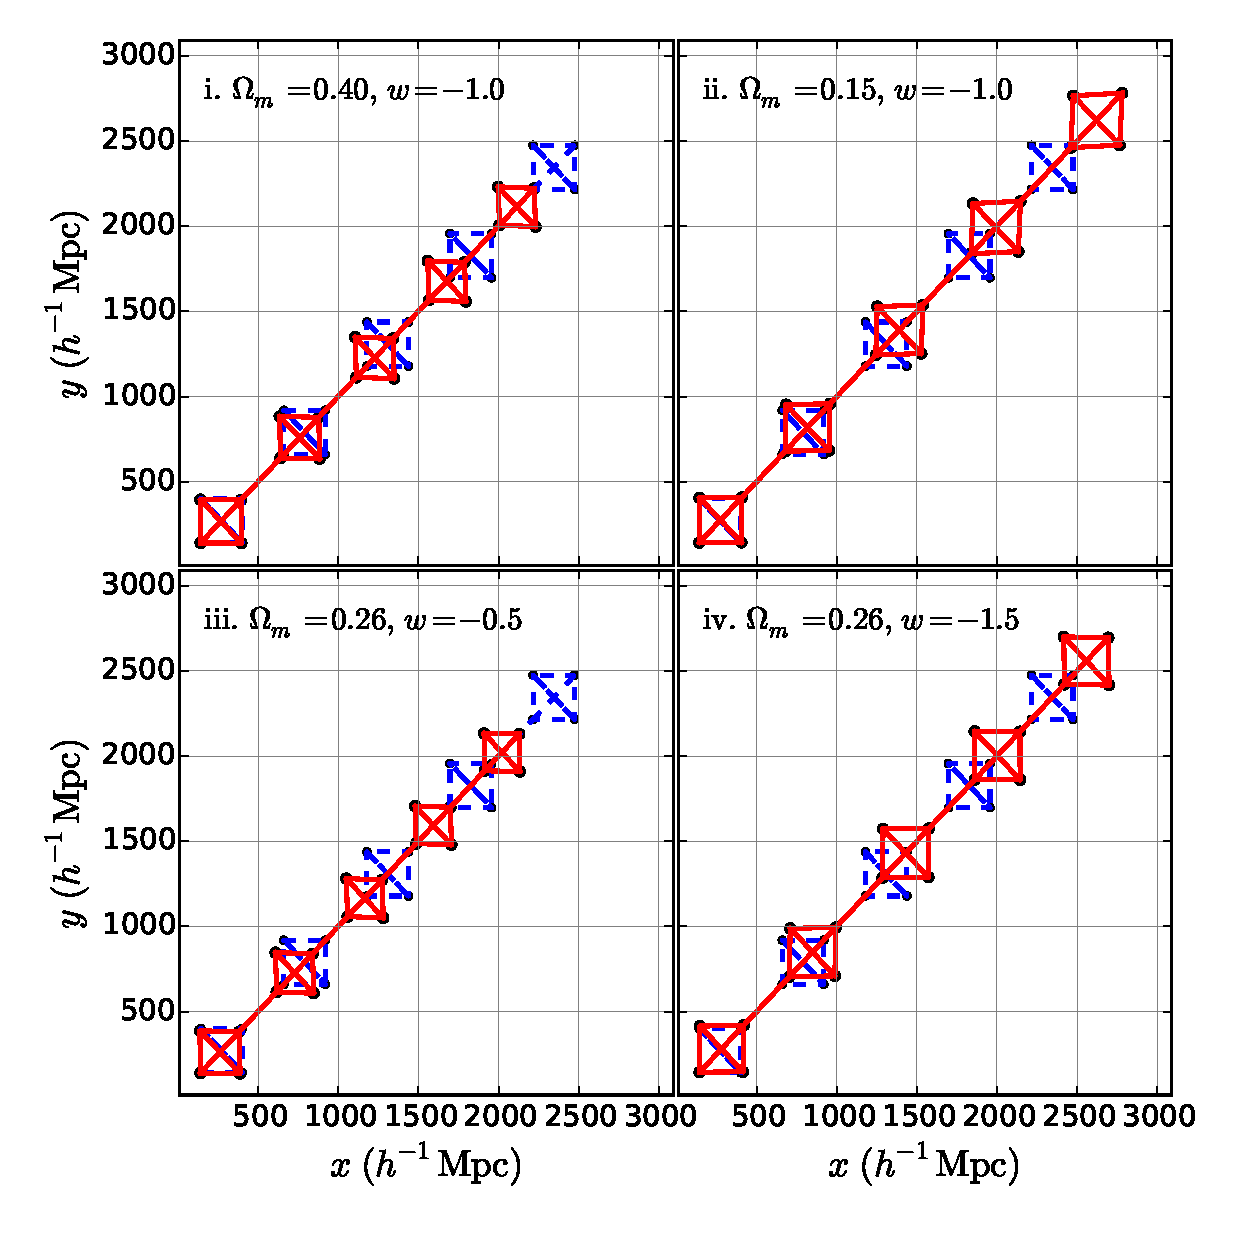
\includegraphics[height=8cm]{fig1_a.eps}
   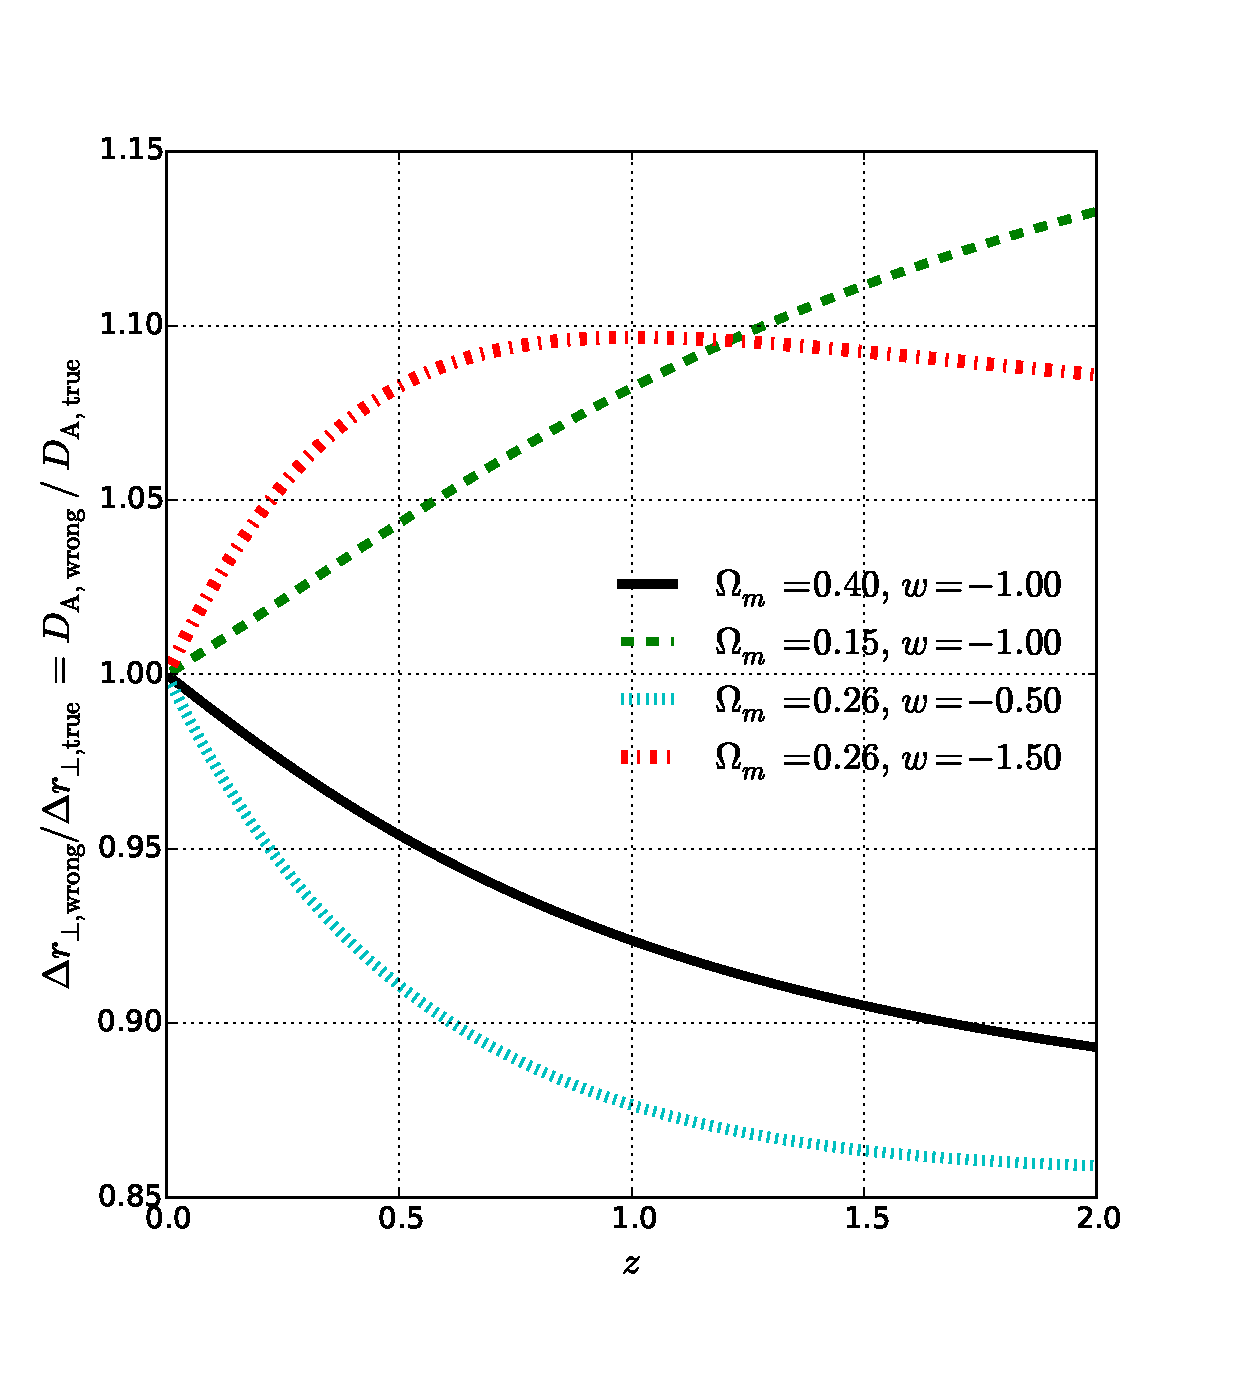
\includegraphics[height=8.5cm]{fig1_b.eps}
   }
   \caption{\label{fig_xyquan}
   A description of how incorrectly assumed cosmologies can distort the interpretation of observation,
   assuming $\Omega_m=0.26,w=-1$ is the true cosmology. 
   Left panel shows a series of five regular squares, measured by an observer at the origin.
   Their true positions and shapes are plotted in blue dashed lines.
   When the observer adopts incorrect cosmologies when computing distances from redshifts and infering the positions and shapes of the squares,
   they obtain distorted shapes (red solid lines).
   Right panel shows the redshift evolution of the wrongly estimated angular diameter distance (divided by the correct value).
   }
   % Need a better plot to show angular size variation!!!
\end{figure*}

%Considering we are Let us consider an object in the universe with certain size and shape.
%Its observed redshift span $\Delta z$ and angular size $\Delta \theta$ are related with the comoving sizes by
In this section we briefly introduce the scaling effect caused by incorrectly assumed cosmological parameters.
A more detailed description has been provided in \cite{Li2014,Li2015,Li2016}.

Suppose that we are probing the size of some objects in the Universe.
We measure their redshift span $\Delta z$ and angular size $\Delta \theta$,
then compute their sizes in the radial and transverse directions using the following formulas
\begin{equation}\label{eq:distance}
\Delta r_{\parallel} = \frac{c}{H(z)}\Delta z,\ \ \Delta r_{\perp}=(1+z)D_A(z)\Delta \theta,
\end{equation}
where $H$ is the Hubble parameter and $D_A$ is the angular diameter distance.
In the particular case of a flat universe composed of a cold dark matter component and a constant EoS dark energy, they take the forms
\begin{eqnarray}\label{eq:HDA}
& &H(z) = H_0\sqrt{\Omega_ma^{-3}+(1-\Omega_m)a^{-3(1+w)}},\nonumber\\
& &D_A(z) = \frac{1}{1+z}r(z)=\frac{1}{1+z}\int_0^z \frac{dz^\prime}{H(z^\prime)},
\end{eqnarray}
where $a=1/(1+z)$ is the cosmic scale factor,
$H_0$ is the present value of Hubble parameter and $r(z)$ is the comoving distance.

When incorrect values of $\Omega_m$ and $w$ are adopted, 
the inferred $\Delta r_{\parallel}$ and $\Delta r_{\perp}$ are also incorrect,
resulting in erroneous estimation of the object's shape (AP effect) and size (volume effect).
These effects and their cosmological consequences have been studied in \cite{Li2014,Li2015,Li2016}.

In this paper we focus on the mis-estimation of the angular size $\Delta r_{\perp}$. %scaling of angular size,
The ratio of mis-estimation is
\begin{equation}\label{eq:DA}
 %{\rm Degree\ of\ volume\ magnification \equiv}
 %{\rm rat}_{\rm volume\ mag}\equiv
 \alpha_{\perp} \equiv \frac{\Delta r_{\perp, \rm wrong}}{\Delta r_{\perp, \rm true}}
 = \frac{D_{A, \rm wrong}}{D_{A, \rm true}},
\end{equation}
where ``true'' and ``wrong'' denote the values in the true cosmology and wrongly assumed cosmologies respectively.

An illustration is provided in the left panels of Figure \ref{fig_xyquan}.
Suppose that the true cosmology is a flat $\Lambda$CDM with present matter ratio $\Omega_m=0.26$
and standard dark energy EoS $w=-1$.
If we were to distribute a series of perfect squares at distances ranging from 500 Mpc/h to 3\,000 Mpc/h,
and an observer located at the origin were to measure their redshifts and infer the sizes of the squares
using the distance-redshift relations of four incorrect cosmologies
\begin{eqnarray}
 & &{\rm (i)}.\ \Omega_m=0.40,\ w=-1.0, \nonumber \\ 
 & &{\rm (ii)}.\ \Omega_m=0.15,\ w=-1.0, \nonumber\\ \noindent
 & &{\rm (iii)}.\ \Omega_m=0.26,\ w=-0.5,\nonumber\\ \noindent
 & &{\rm (iv)}.\ \Omega_m=0.26,\ w=-1.5,  \nonumber \noindent 
\end{eqnarray}
then the shapes of the squares would appear distorted (AP effect),
and their sizes would be wrongly estimated (volume effect).
Cosmological models (i,iii) result in compressed volume elements (in both angular and LOS directions),
and the degree of compression increases with increasing distance;
the situation is opposite for the other two cosmologies.

The mis-estimation of angular size, ${\Delta r_{\perp, \rm wrong}}/{\Delta r_{\perp, \rm true}}$, 
is displayed in the right panel of Figure \ref{fig_xyquan}.
In all cosmologies, ${\Delta r_{\perp, \rm wrong}}/{\Delta r_{\perp, \rm true}}$ evolves significantly in the redshift range $0\leq z\leq 2$.
As an example, when adopting the quintessence cosmology $\Omega_m=0.26,\ w=-0.5$,
the angular size is underestimated by 
%12.5\%, 17.7\%, 20.1\%, 21.3\%
8.9\%, 12.3\%, 13.6\%, 14.1\% 
at $z=0.5,1,1.5,2$.

%Thus, when wrong cosmological parameters are adopted,
%the apparent size of objects are distorted, and the magnitude of distortion also varies with redshift.

In sum, as a consequence of incorrect cosmologies 
the size of objects is mis-estimated and the magnitude of mis-estimation depends on the redshift.
We use the galaxy 2pCF across the line-of-sight to probe the mis-estimation of angular size, ${\Delta r_{\perp, \rm wrong}}/{\Delta r_{\perp, \rm true}}$.


\section{The Simulation Data}\label{sec:data}

We test the method using the mock galaxy samples produced by the Horizon Run 4  (HR4) N-body simulation \citep{hr4,hong2016}.

HR4 was made within a cube of volume $({3.15}\ h^{-1}\rm Gpc)^3$ using  $6300^3$ particles with mass $m_p\simeq 9 \times 10^9 \hMsun$.
The simulation adopted the second order Lagrangian perturbation theory (2LPT) initial conditions at $z_{i}=100$
and a WMAP5 cosmology $(\Omega_{b},\Omega_{m},\Omega_\Lambda,h,\sigma_8,n_s)$  = (0.044, 0.26, 0.74, 0.72, 0.79, 0.96) \citep{komatsu 2011}.
%The particle mass is $\simeq m_{p} \simeq 9.02 \times 10^9 \hMsun$.
%This starting redshift, combined  with 2LPT initial conditions, ensures an accurate mass function and power spectrum \citep{2014NewA...30...79L}. 

Mock galaxies are produced from the simulation based on a modified one-to-one correspondence scheme \citep{hong2016}. 
The most bound member particles (MBPs) of simulated halos are adopted as tracers of galaxies.
The merger timescale is computed to obtain the lifetime of merged halos.
Merger trees of halos are constructed by tracking their MBPs from $z = 12$ to 0;
when a merger event occurs, the merger timescale is computed using the formula of \cite{jiang2008} to 
determine when the satellite galaxy is completely disrupted.
%We modeled the position and the velocity of a galaxy from the position and velocity of its corresponding MBP.
%By using the abundance matching, 
%we modeled the luminosity of a central/isolated galaxies from their current mass
%and of satellite galaxies from their mass at the time of infall.

The resulting mock galaxies were found to reproduce the 2pCF of the SDSS DR7 volume-limited galaxy sample \citep{zehavi2011} very well.
The mock galaxies shows a similar finger of god (FOG) feature \citep{FOG} as the observation.
The projected 2pCF of the mock and observational samples agree within 1$\sigma$ CL
on scales greater than 1 ${h^{-1}}$Mpc.

%As will be introduced in the next section, 
%The output of HR4 simulation includes one all-sky light cone mock galaxy catalogue reaching $r=3\,150$ ${h^{-1}}$Mpc 
%and a series ({\bf how many?}) of snapshot mock galaxy catalogues at different redshifts.
We take the snapshot data of the mock galaxies at $z=0,0.5,1,1.5,2$.
%We require subhalos to have at least 30 member particles, 
%so the minimal mass of galaxies is $\simeq m_{p} \simeq 2.7 \times 10^{11} \hMsun$.
Setting a minimal halo mass of $3\times 10^{11} \hMsun$, 
%$4.57\times 10^8$, $4.06\times 10^8$, $3.52\times 10^8$, $3.06\times 10^8$ and $2.28 \times 10^8$ mock galaxies,
we select 457, 406, 352, 306 and 228 million mock galaxies at the five redshifts,
corresponding to a number density of 
%$1.46\times 10^{-2}$, $1.30\times 10^{-2}$, $1.13\times 10^{-2}$, $0.98\times 10^{-2}$ and $0.73\times 10^{-2}\ (h^{-1} \rm Mpc)^{-3}$,
1.46, 1.30, 1.13, 0.98 and 0.73 in units of $ 10^{-2} h^{3} \rm Mpc^{-3}$
%$1.46\times 10^{-2}$, $1.30\times 10^{-2}$, $1.13\times 10^{-2}$, $0.98\times 10^{-2}$ and $0.73\times 10^{-2}\ (h^{-1} \rm Mpc)^{-3}$,
respectively.
Applying a uniform mass cut, at higher redshift we obtained a smaller number of galaxies with {\it larger bias}.

As an illustration, Figure \ref{fig_scatter} displays the 2D distribution of a subsample of mock galaxies in five redshifts,
with $x$, $y$ coordinates computed using the ``correct'' cosmological parameters $\Omega_m=0.26,\ w=-1$ (left panels) 
and a set of wrong cosmological parameters $\Omega_m=0.05,\ w=-1.5$ (right panels), respectively.

When the correct cosmology is adopted the cosmic scale is correctly estimated,
the main factor leads to redshift evolution of galaxy distribution is the gravitational growth of structure.
With decreasing redshift, we clearly see the clusters and filaments form and grow.
On the other hand, when the wrong cosmology is adopted, there is an artificial scaling of distances in the constructed map.
The separations among galaxies are over-estimated by 
$25.6\%,47.3\%,62.2\%,71.7\%$ at redshifts of $0.5,1.0,1.5,2.5$,
leading to a clear redshift evolution of sizes of structures.

The growth of structure increases the clustering and results in more compact structures,
while the volume effect maintains the clustering pattern and uniformly re-scales structures on all scales.
The imprint of each of these effects on the large scale structure is different and should be distinguishable.
In the following section we show that they affect $\xi(r_{\bot})$ measurements in different ways, 
and thus can be easily separated.

%The growth of structure also make the size of structures evolves with redshift.
%In the next subsection we will discuss how to distinguish these two effects in the galaxy angular 2pCF.


%The left panels of Figure \ref{fig_scatter} show the $x,y$ coordinates of galaxies in a 
%$260 h^{-1} {\rm Mpc} \times 130 h^{-1} {\rm Mpc} \times 105 h^{-1} {\rm Mpc}$ volume, 
%taken from the five snapshots.
%The gravitational growth of structures with decreasing redshift is clearly shown.
%We display all mock galaxies with $M> 3.0 \times 10^{11} \hMsun$.
%At lower redshift, galaxies become more massive, so they are more galaxies satisfying the threshold.

%If one adopts a wrong cosmology to compute galaxy positions, there would be a scaling of the galaxy distribution.
%In the left panel we show the case when a wrong set of parameters $\Omega_m=0.05,\ w=-1.5$ is assumed,
%leading to large upscaling of $25.6\%,47.3\%,62.2\%,71.7\%$ at redshifts $z=0.5,1.0,1.5,2.5$.

%Compared with the true galaxy distribution, the apparent distribution inferred by wrong set of parameters
%show clear evolution with redshift due to the different scaling at different redshifts.
%In case of Figure \ref{fig_scatter}, the apparent size of large scale structures increases with redshift.

%The growth of structure also make the size of structures evolves with redshift.
%In the next subsection we will discuss how to distinguish these two effects in the galaxy angular 2pCF.

\begin{figure*}
   \centering{
   %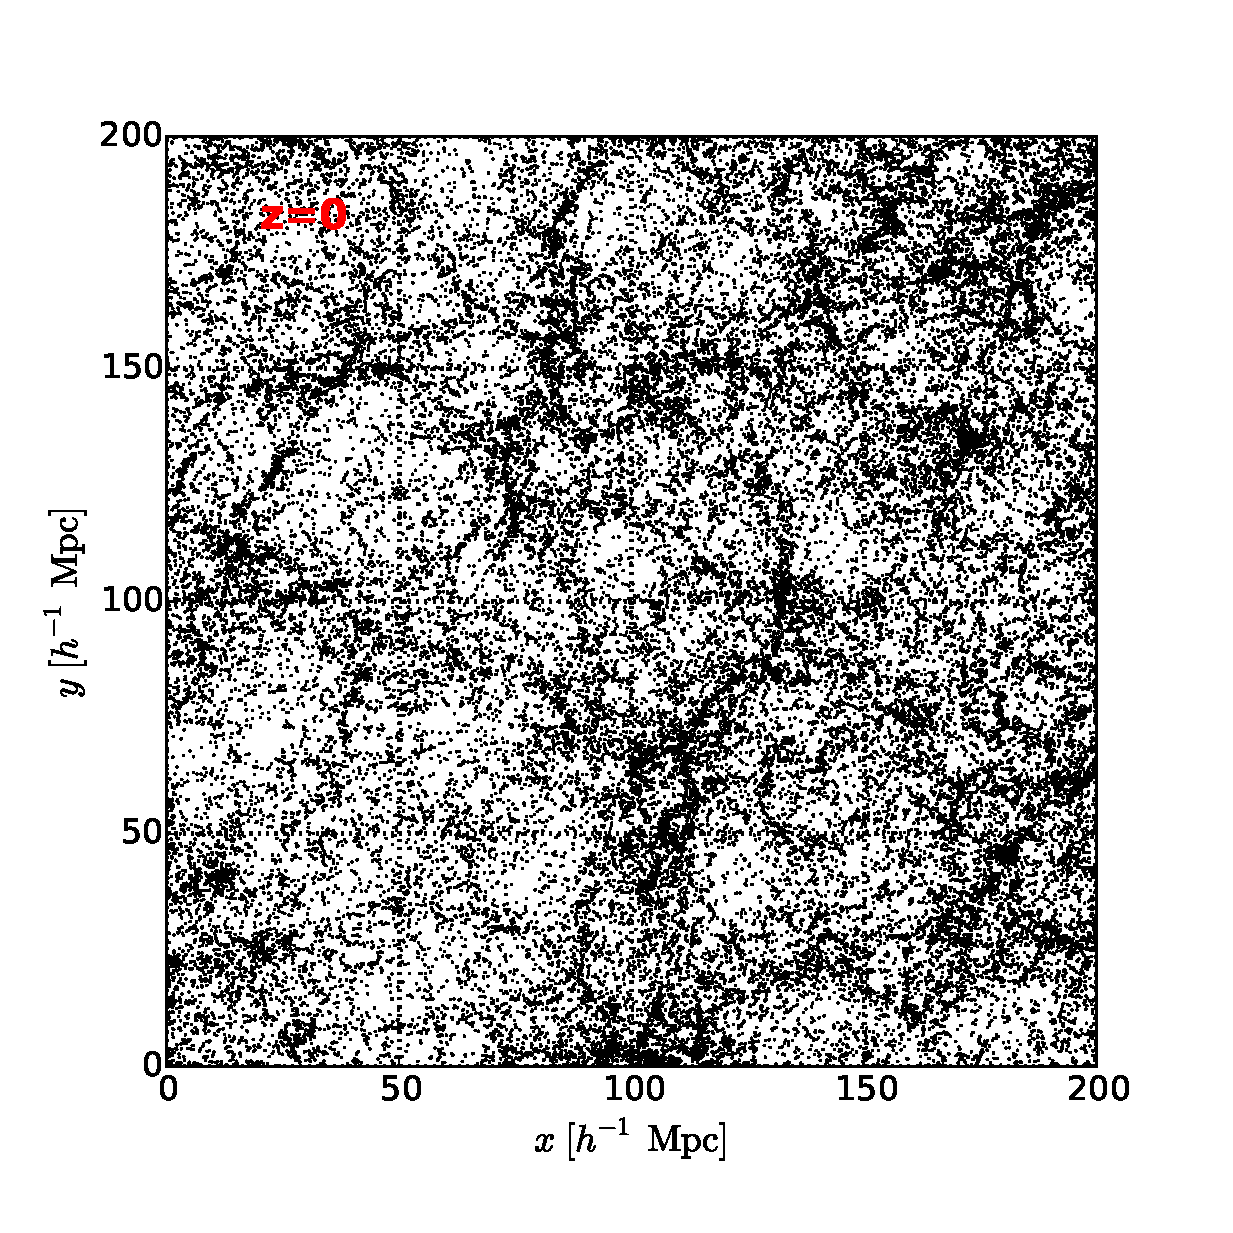
\includegraphics[height=5.9cm]{fig8_0.eps}
   %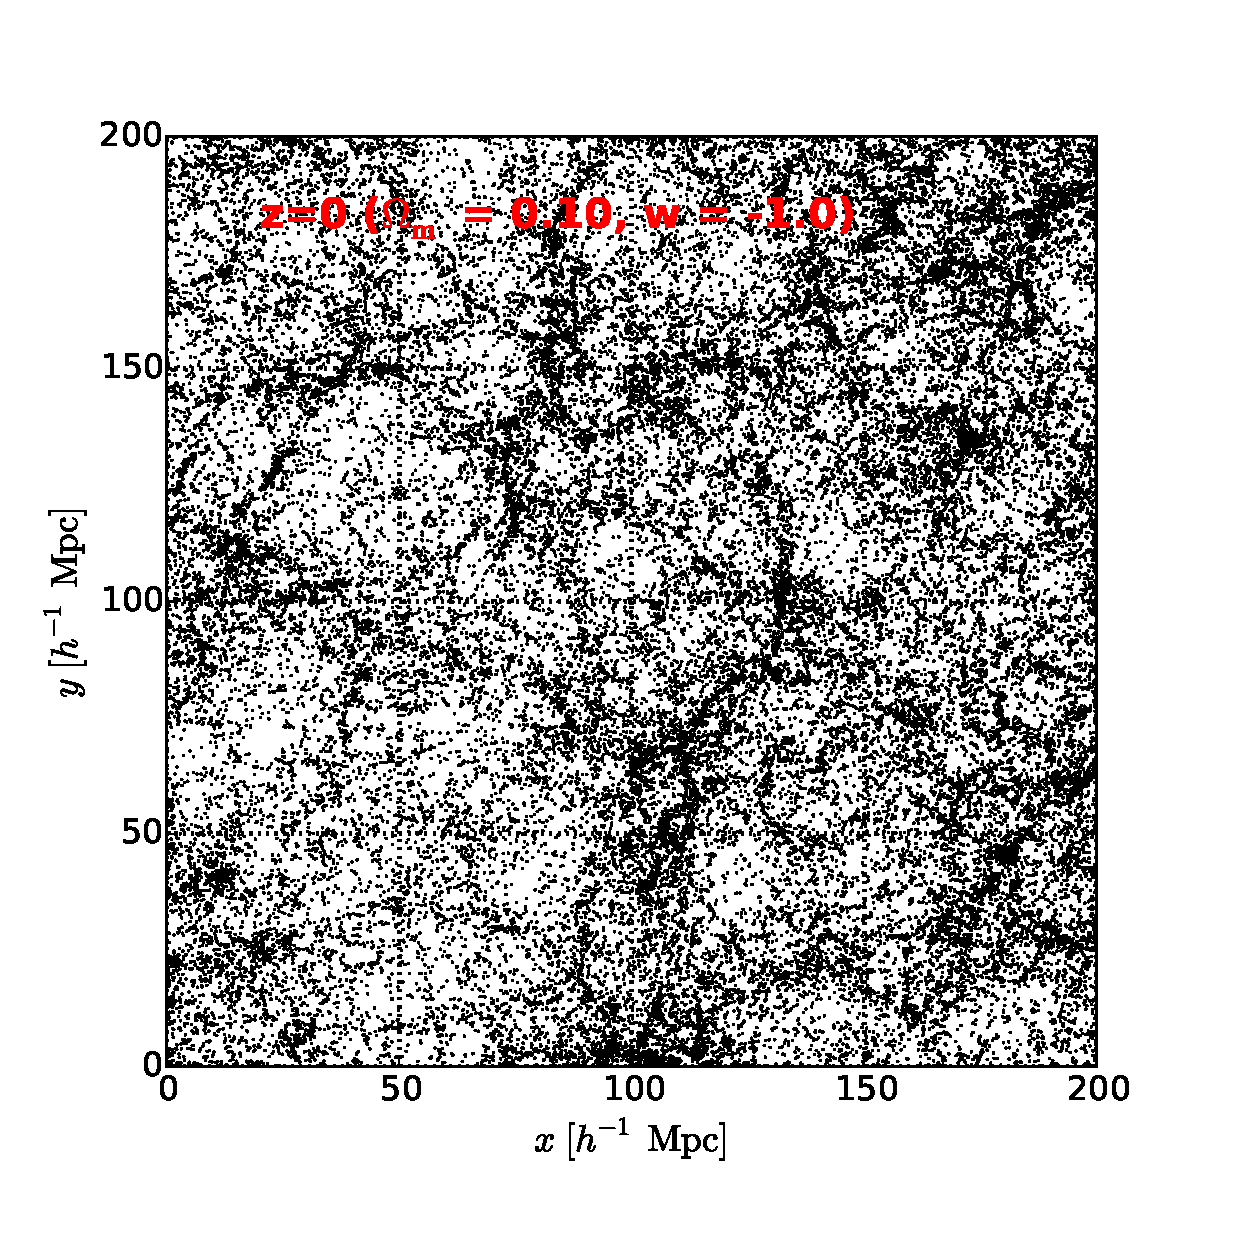
\includegraphics[height=5.9cm]{fig8_wrongcos_0.eps}
   %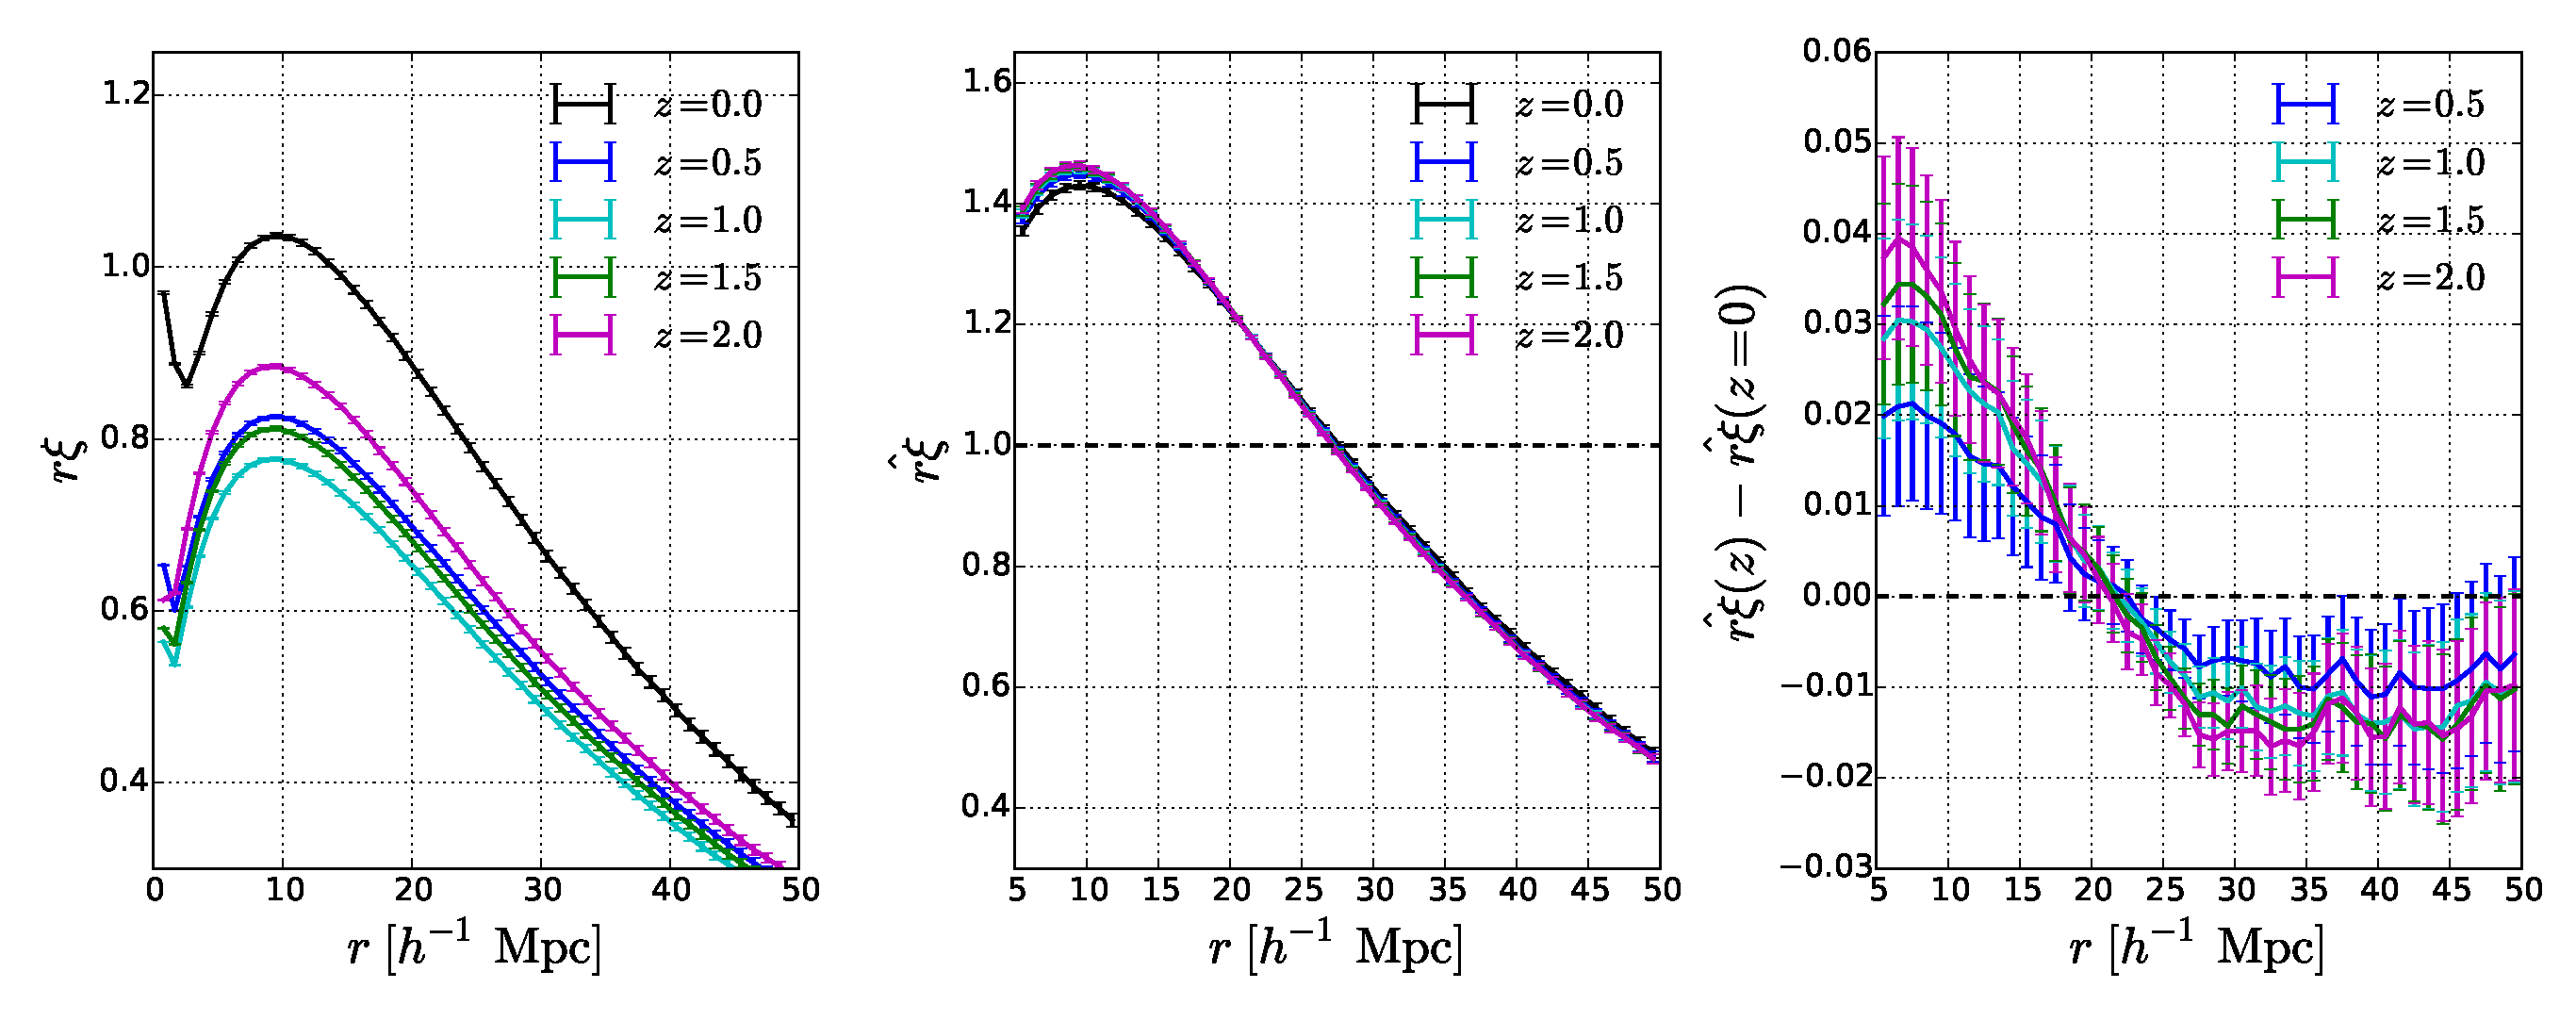
\includegraphics[width=16cm]{fig2.eps}
   %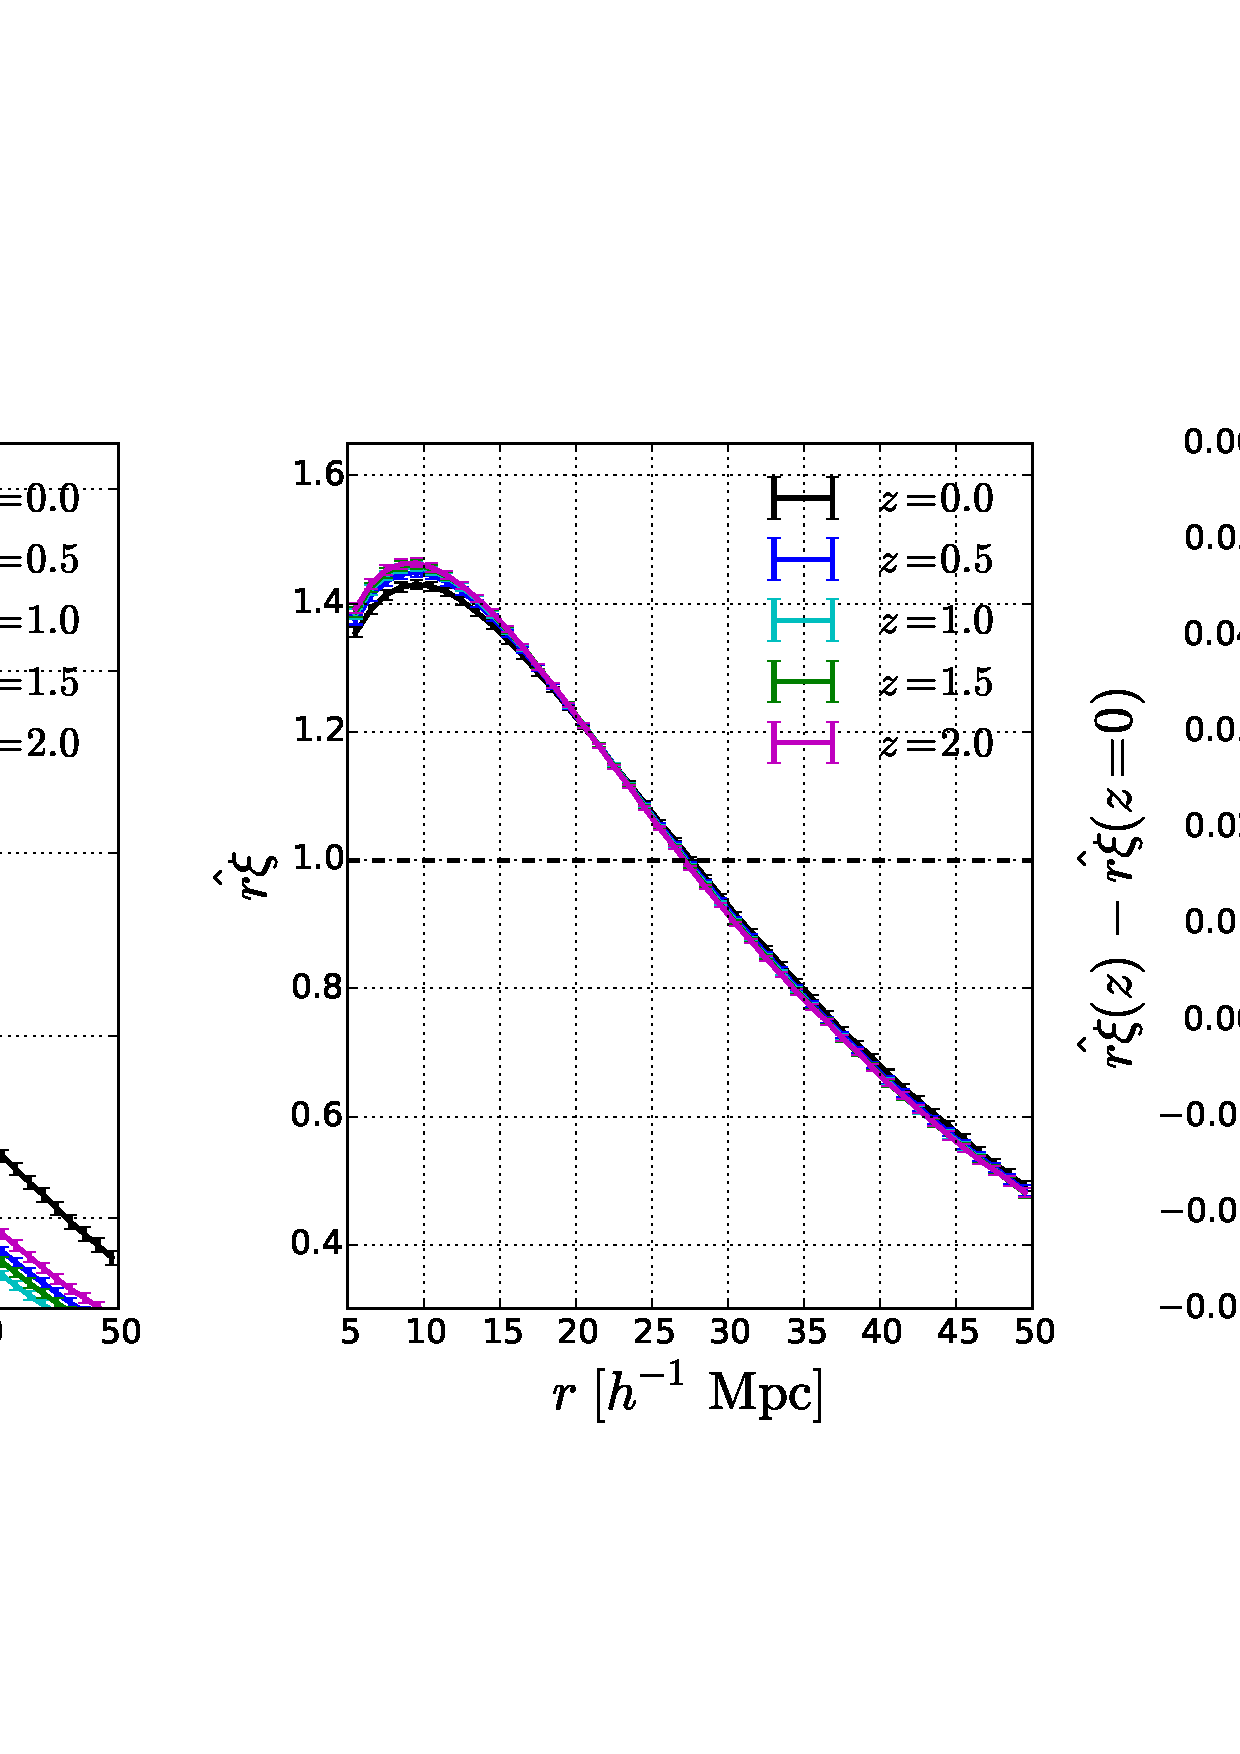
\includegraphics[width=16cm,natwidth=8,natheight=14]{fig2.pdf}
   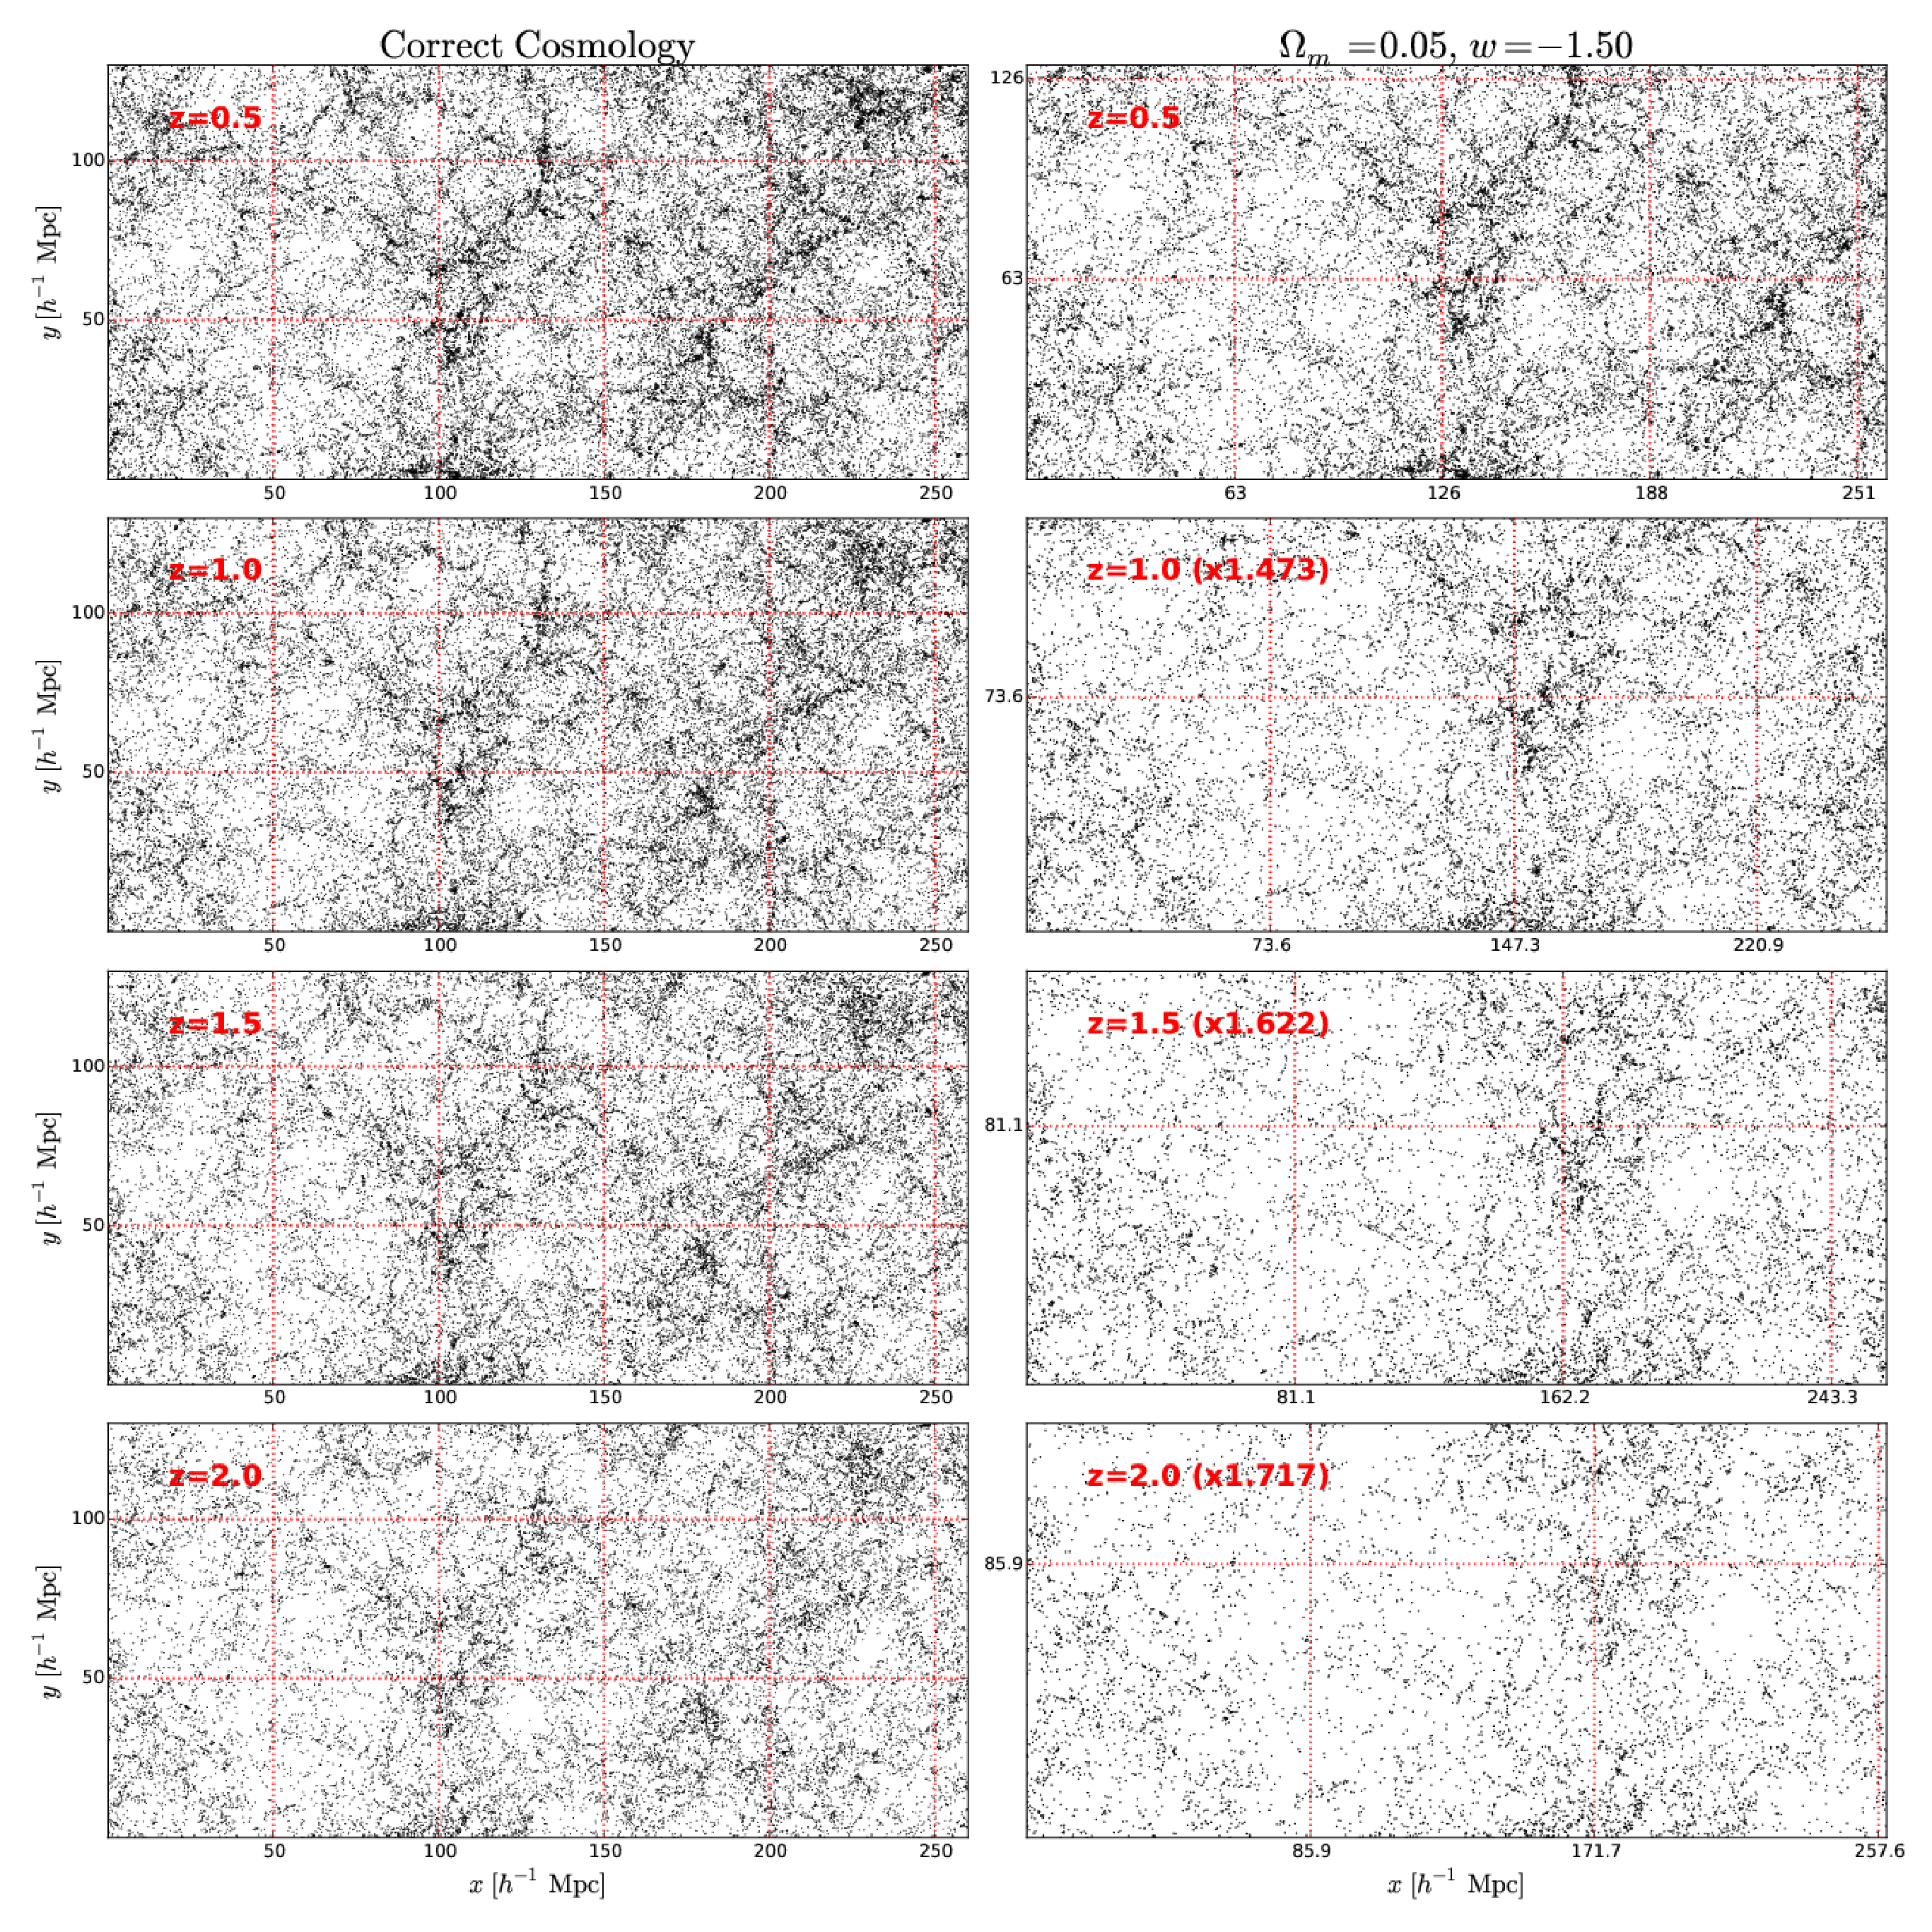
\includegraphics[width=16cm]{fig2_0.eps}
   }
   \caption{\label{fig_scatter}
  The 2D distribution of a $260\times130\times105 (h^{-1}{\rm Mpc})^3$ subsample of HR4 mock galaxies, 
  at redshifts 0.5, 1, 1.5 and 2.
  Left and right panels show the $x$, $y$ coordinates computed using the ``correct'' parameters $\Omega_m=0.26,\ w=-1$ 
  and a set of wrong cosmological parameters $\Omega_m=0.05,\ w=-1.5$, respectively.
  The growth of structure strengths the clustering and make structures more compact at lower redshift.
  When the wrong cosmology is adopted, the comoving distances are mis-scaled and over-estimated by $25.6\%,47.3\%,62.2\%,71.7\%$ at redshifts of $0.5,1.0,1.5,2.5$, respectively,  leading to a clear redshift evolution of the sizes of structures.
   }
   % Need a better plot to show angular size variation!!!
\end{figure*}

\section{Methodology}

%\subsection{Galaxy distribution at different redshifts}

We use the 2pCF across the line-of-sight as a statistical tool to probe the volume effect.
The galaxy 2pCF as a function of galaxy separation perpendicular to the LOS, $\xi(r_\perp)$, is computed for snapshot data of mock galaxies at redshifts 0.5, 1, 1.5 and 2.
We adopt the Landy-Szalay estimator~\citep{1993ApJ...412...64L},
\begin{equation}
\xi(r_\perp)=\frac{DD-2DR+RR}{RR}\ ,
\end{equation}
where $DD$ is the number of galaxy--galaxy pairs, 
$DR$ the number of galaxy-random pairs, 
and $RR$ is the number of random--random pairs, 
all separated by a distance defined by $r_\perp\pm\Delta_{r_\perp}$ where we choose $\Delta_{r_\perp}=1h^{-1}\rm Mpc$.
The random catalogue consists of unclustered points uniformly distributed in the same space as the simulated data. 
In an effort to reduce the statistical variance of the estimator, we use 50 times as many random points as we have galaxies.

Considering the large number of galaxies and random points the 2pCF is computed part by part in subsamples with 
size of 1575 $h^{-1}{\rm Mpc}\times 1575\ h^{-1}{\rm Mpc}\times 105\ h^{-1}{\rm Mpc}$.
The `sheet'-like shape of the subsample is similar to the shape of redshift shells in the real observational case.
The Z direction with thickness $105\ h^{-1}\rm Mpc$ is treated as the radial direction (the $r$ direction) 
and the X-Y directions %with each of width $1575 h^{-1}\ \rm Mpc$ 
are the angular plane.
For our simulation box size we have 120 such subsamples.
The average of the measurements in all subsamples is taken as the 2pCF of the whole sample,
while the covariances of them are taken to be the covariance matrix (after multiplying by a factor of $1/\sqrt{119}$).


\subsection{Galaxy 2pCF across the line-of-sight: at different redshifts}\label{sec_2pCF_diffz}

\begin{figure*}
   \centering{
%   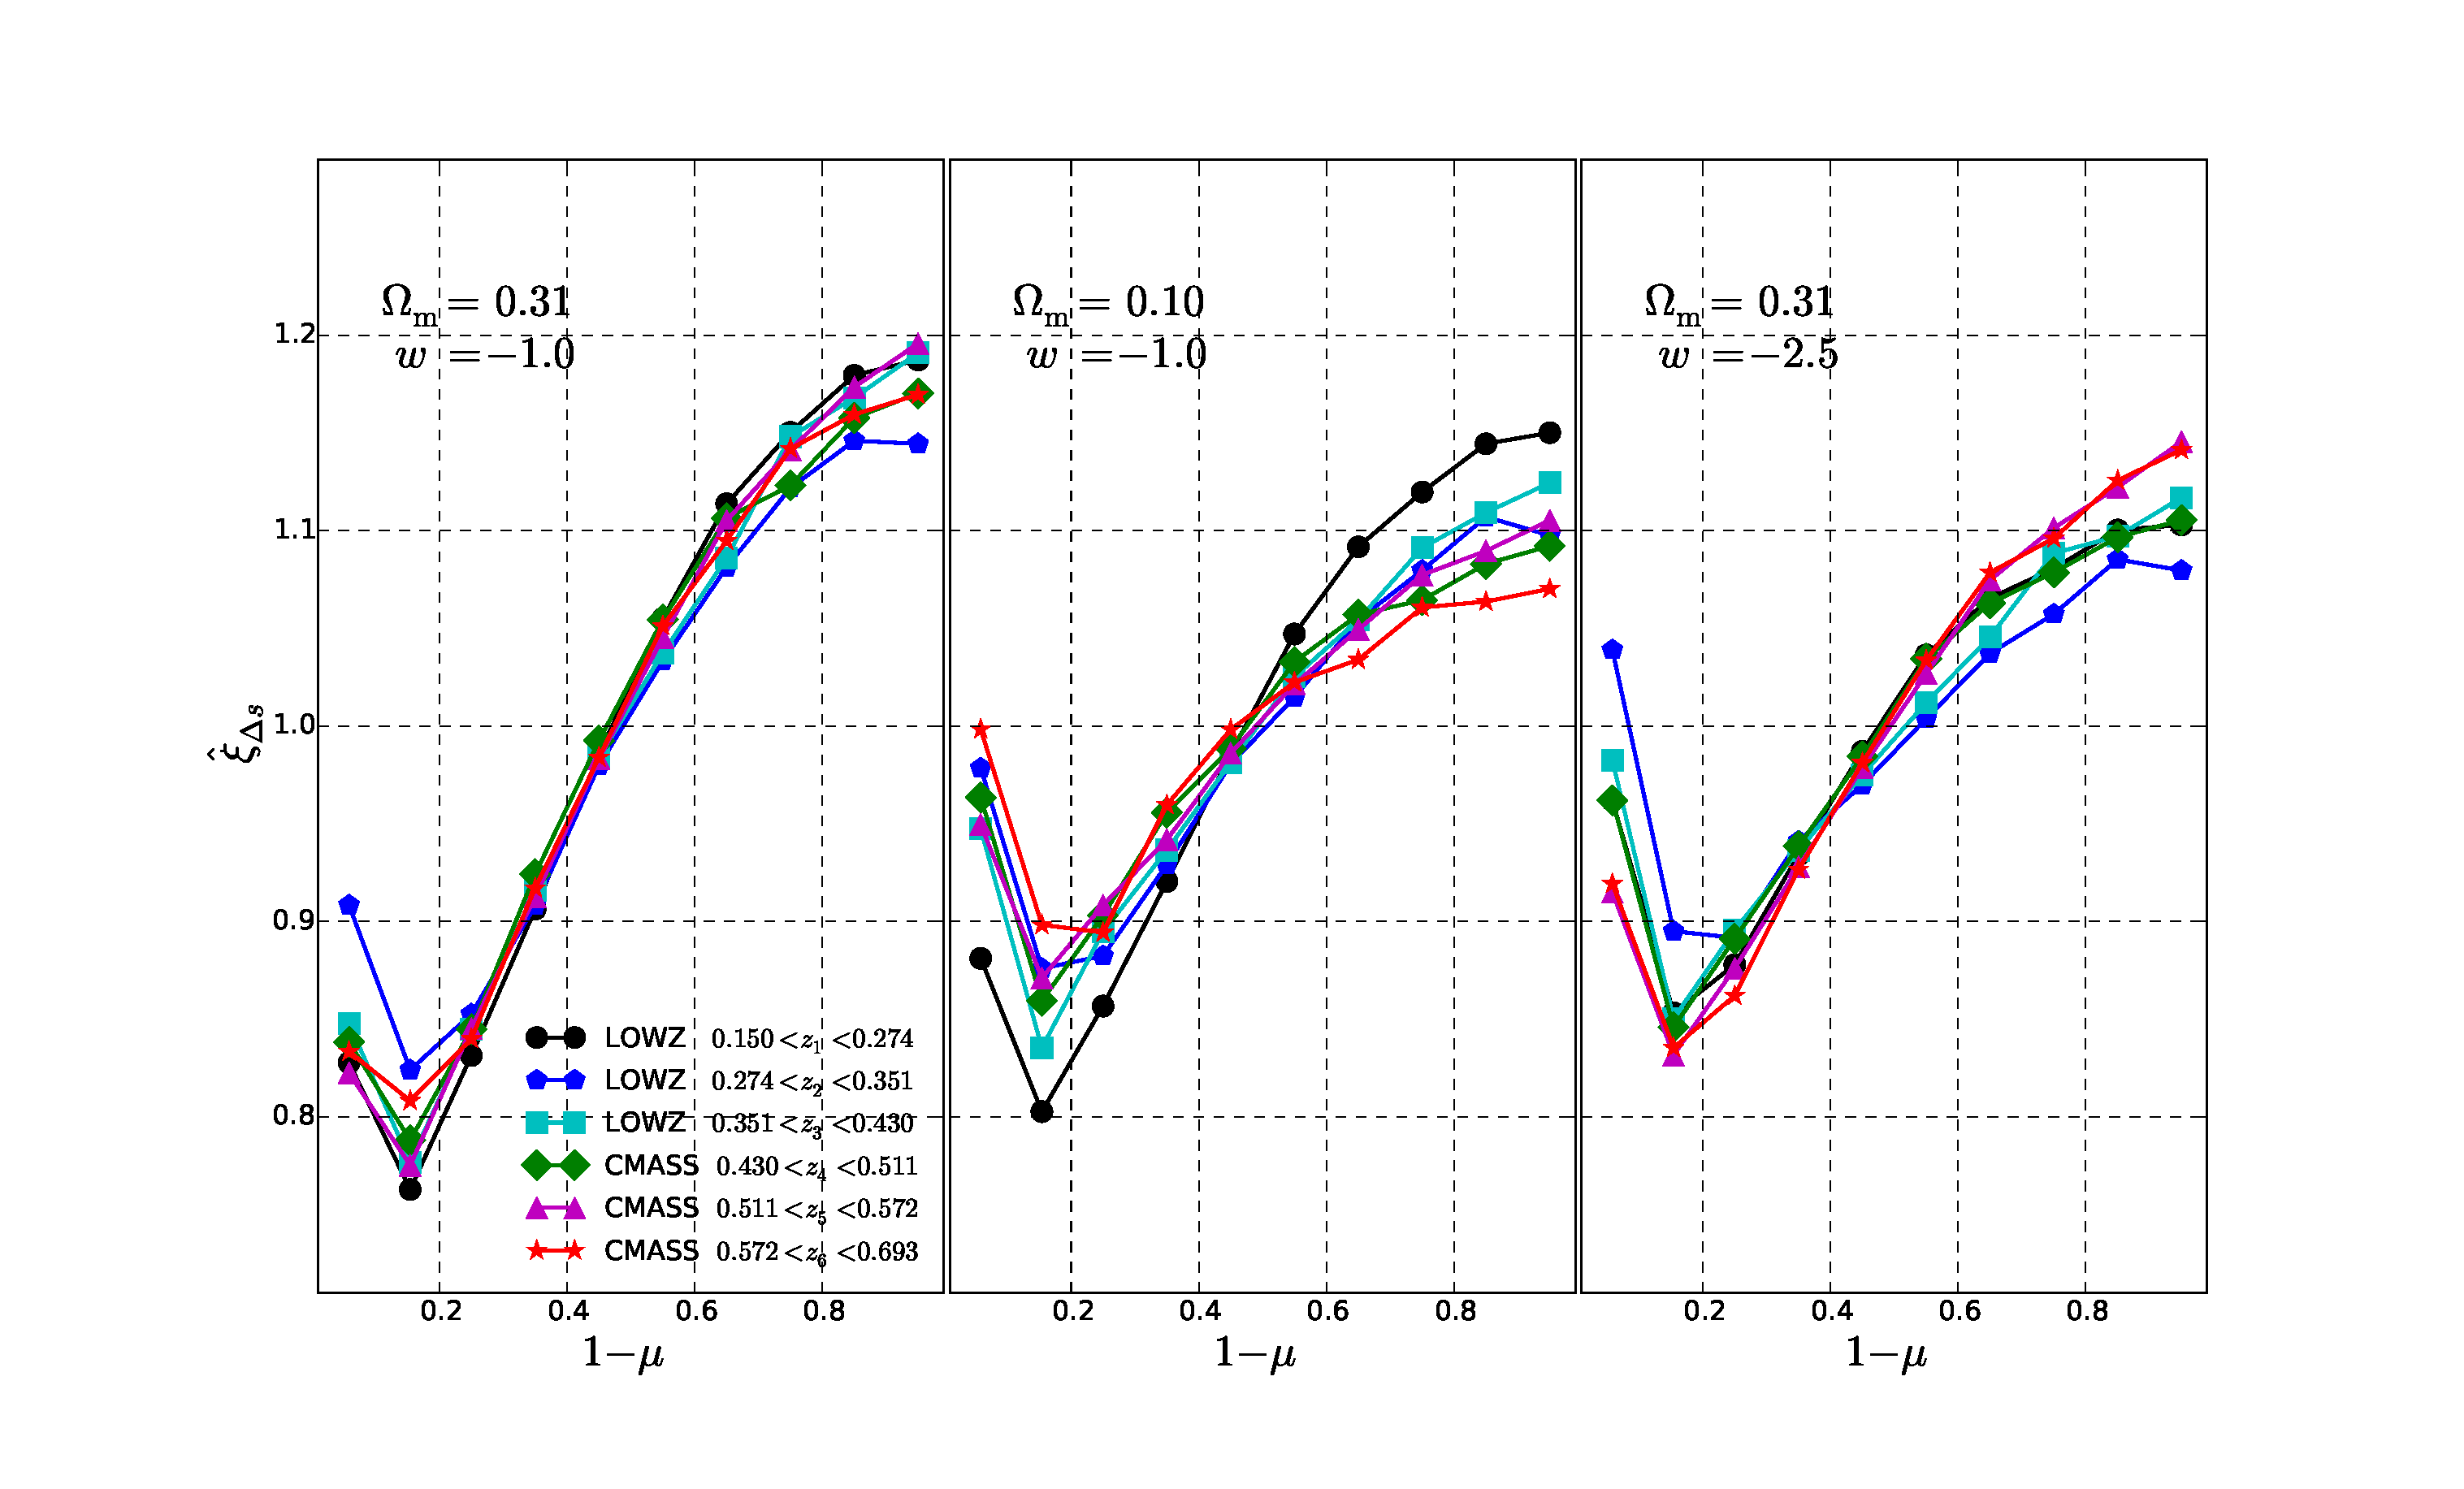
\includegraphics[width=18cm]{fig9_0.eps}
%   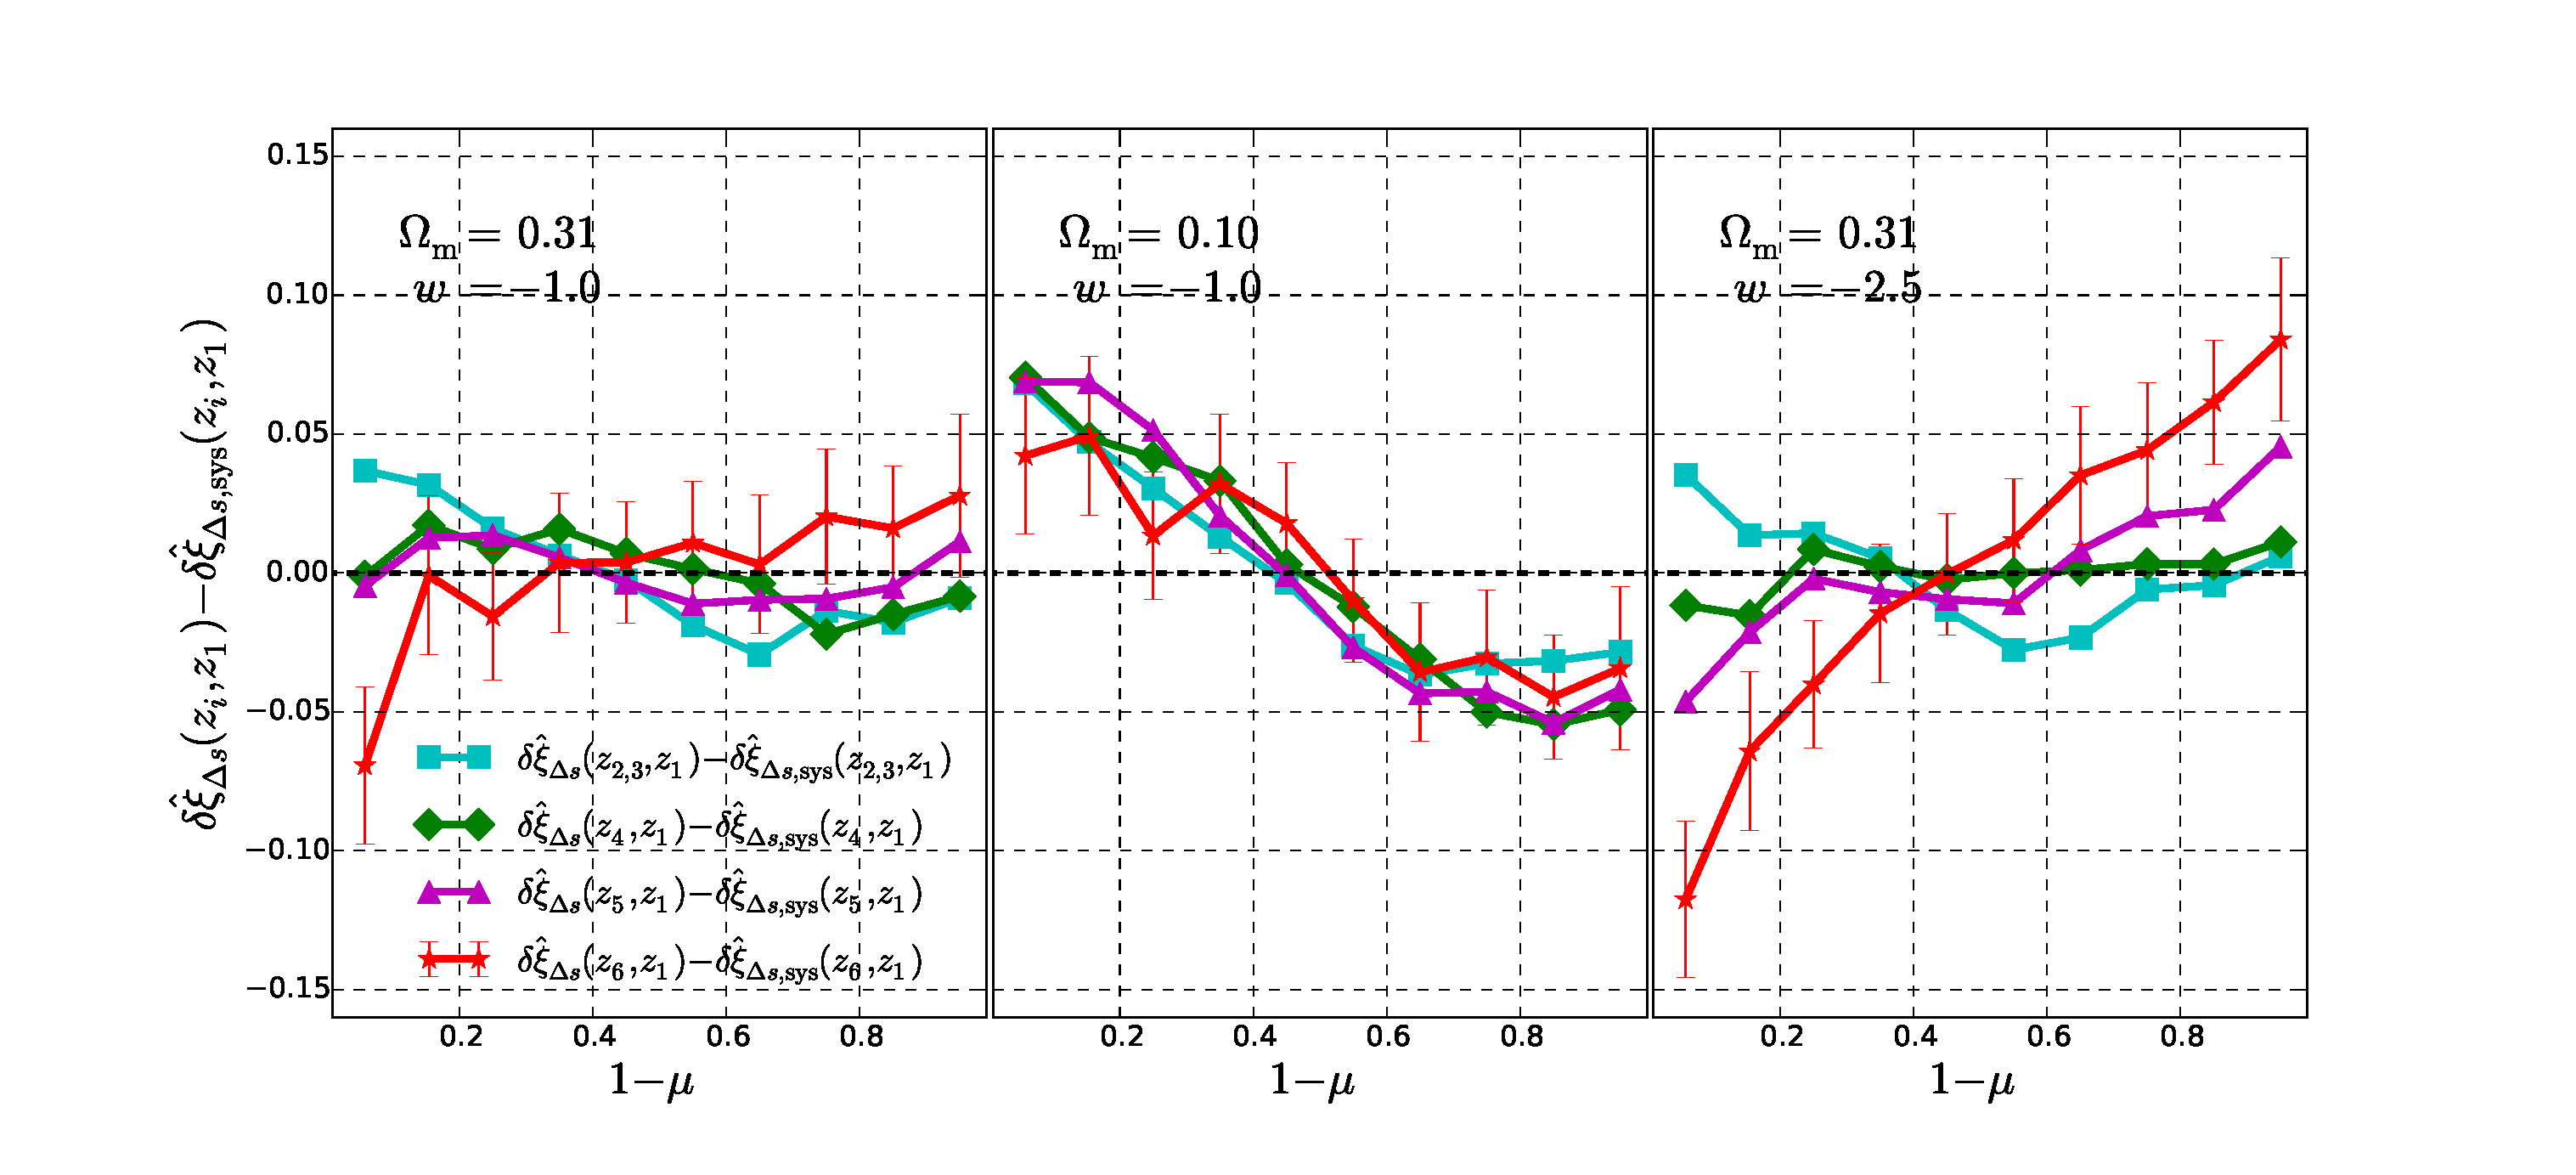
\includegraphics[width=18cm]{fig9_1.eps}
%   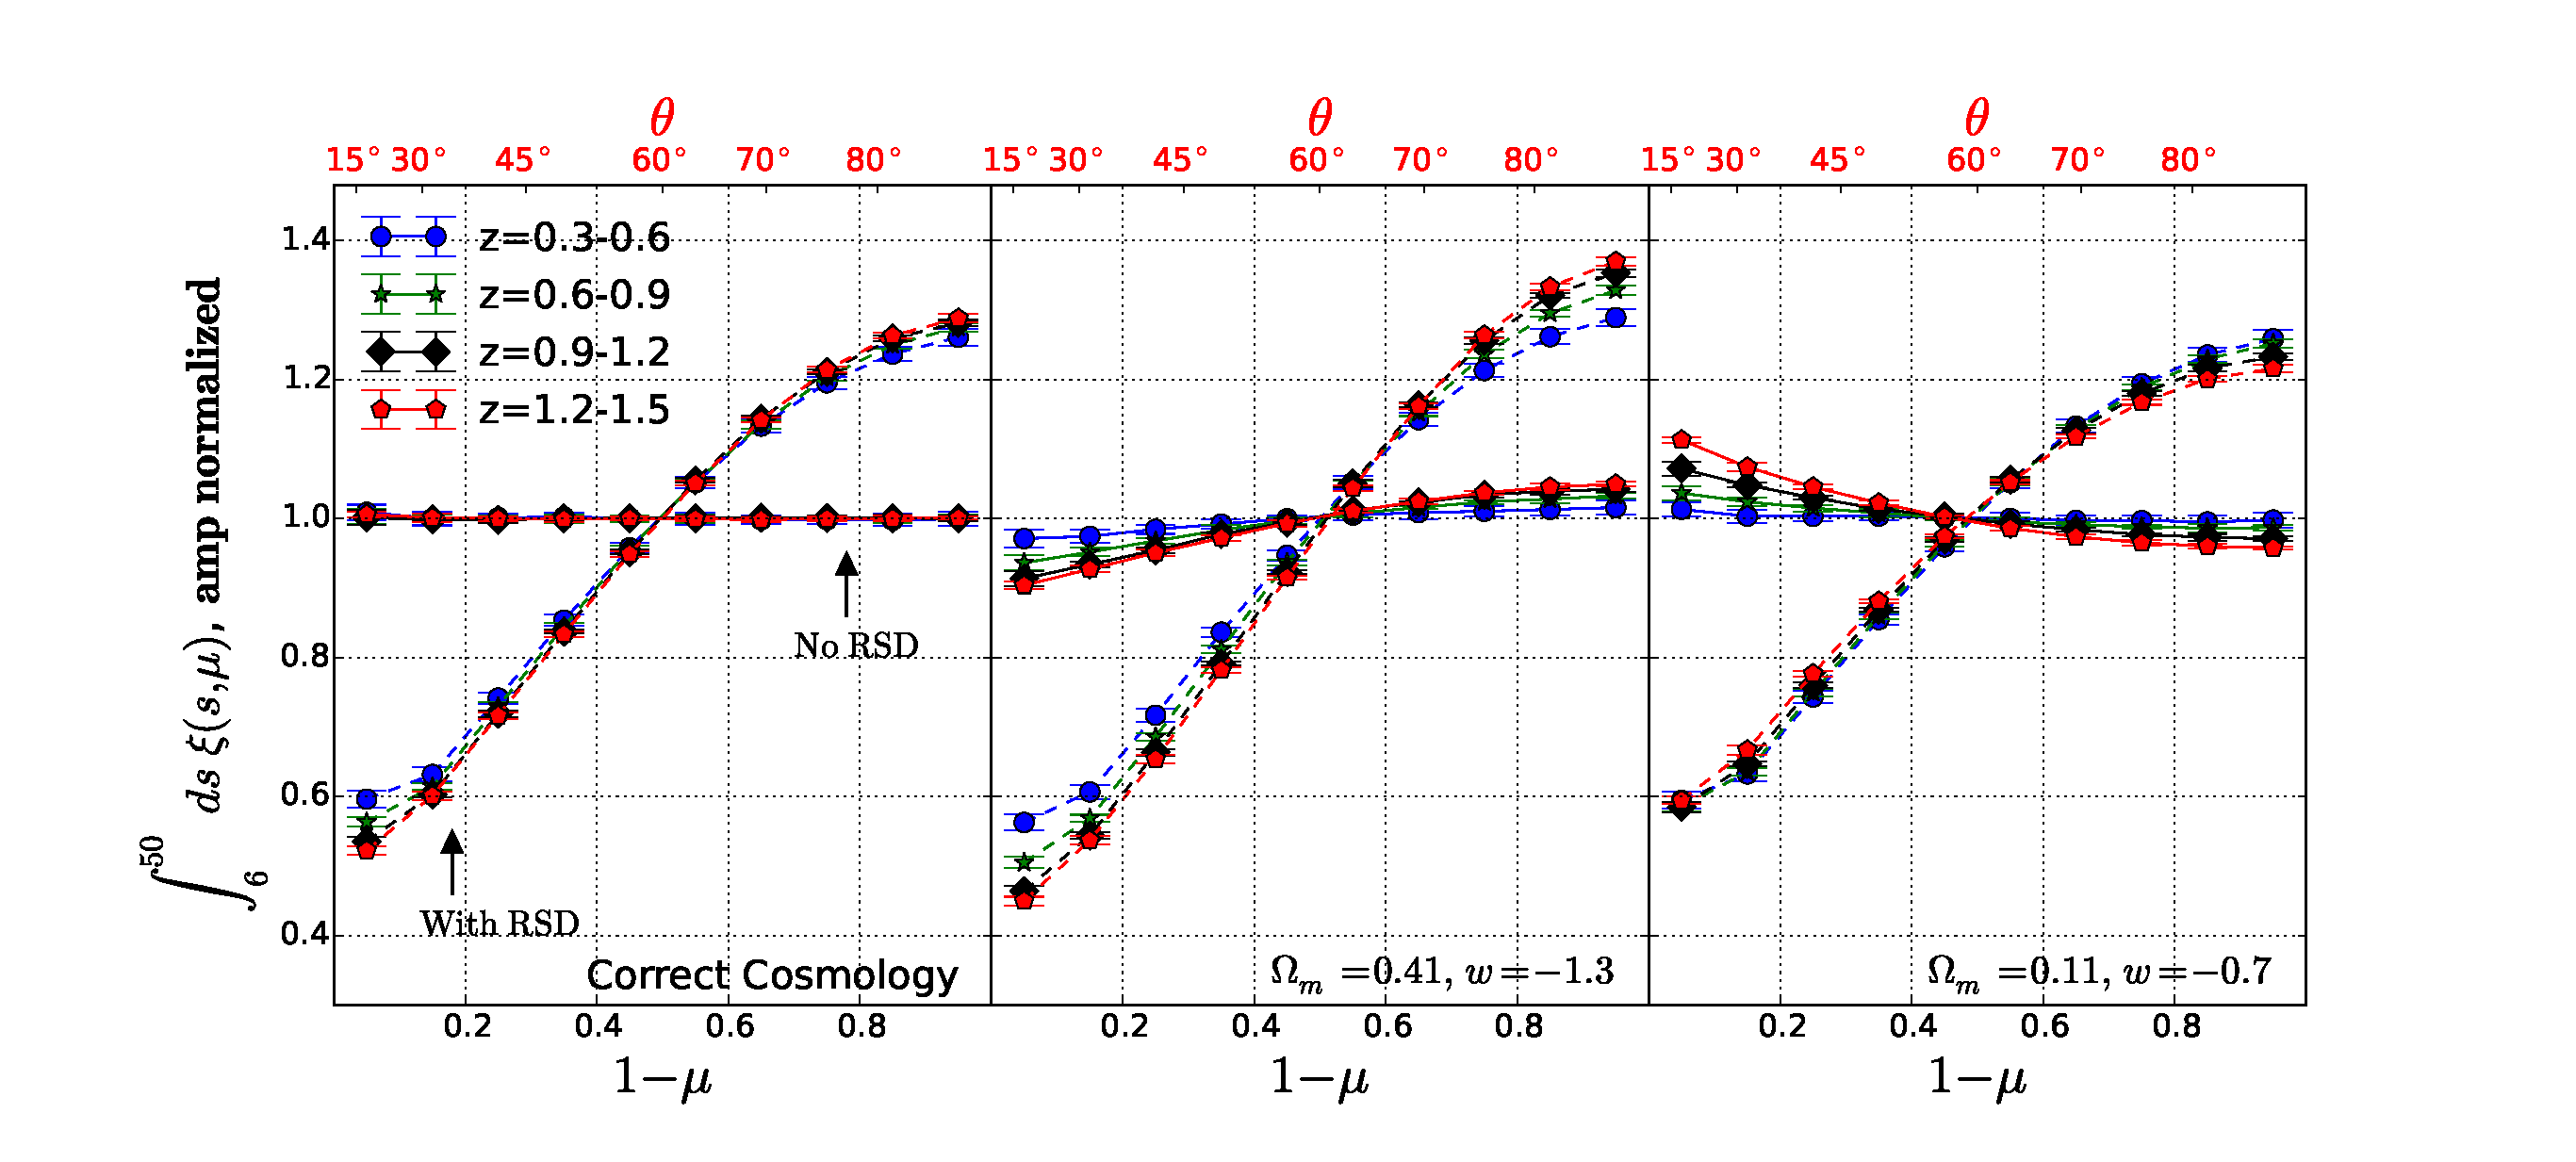
\includegraphics[height=8cm]{Tpcf--plot--Normed.eps}
%    \includegraphics[height=8cm]{smu.eps}
 %   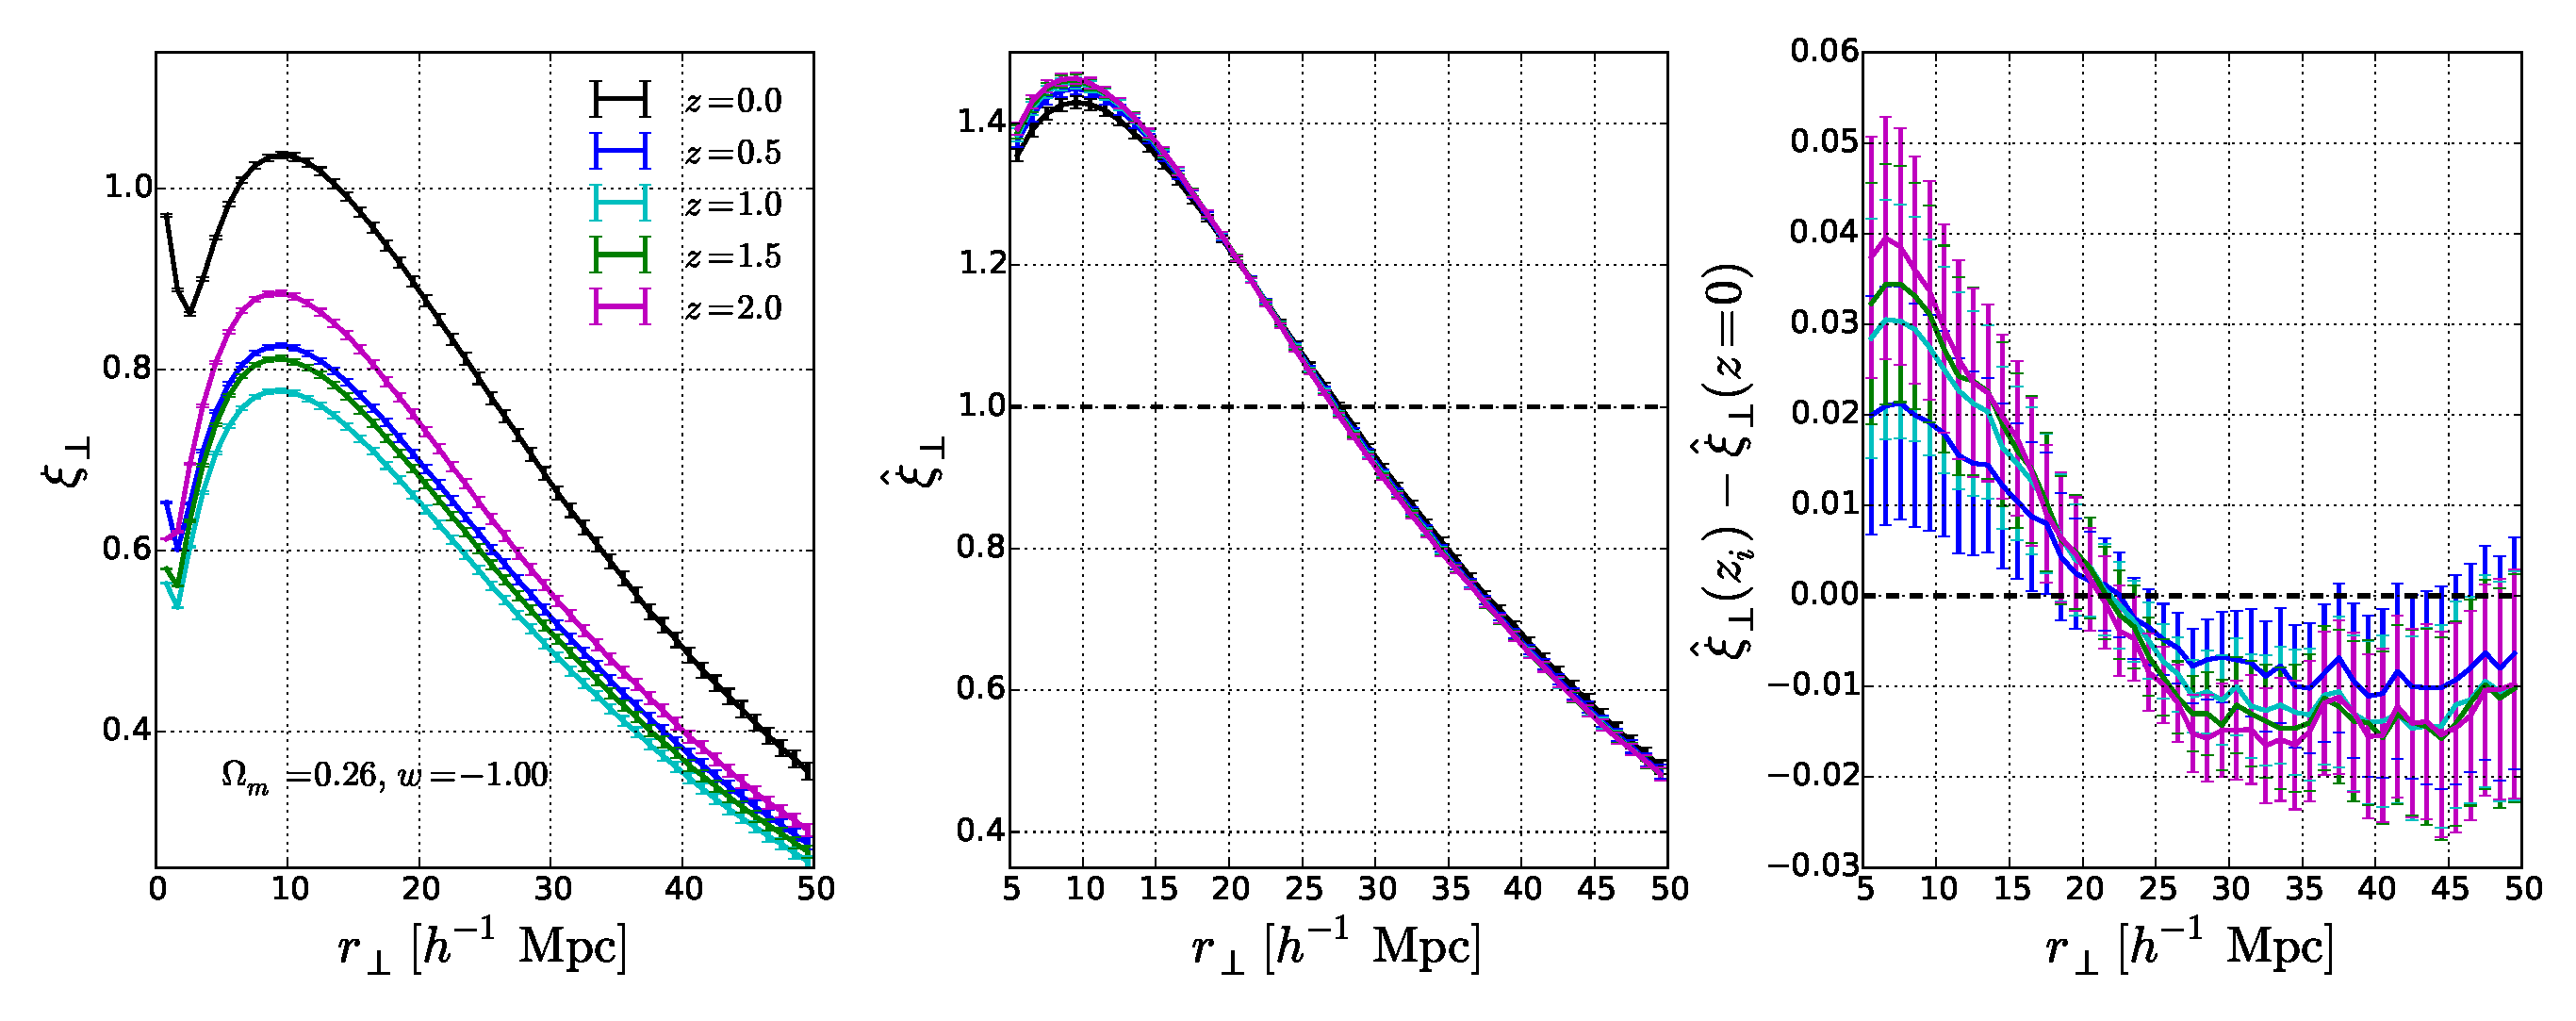
\includegraphics[width=18cm]{fig3.eps}
%    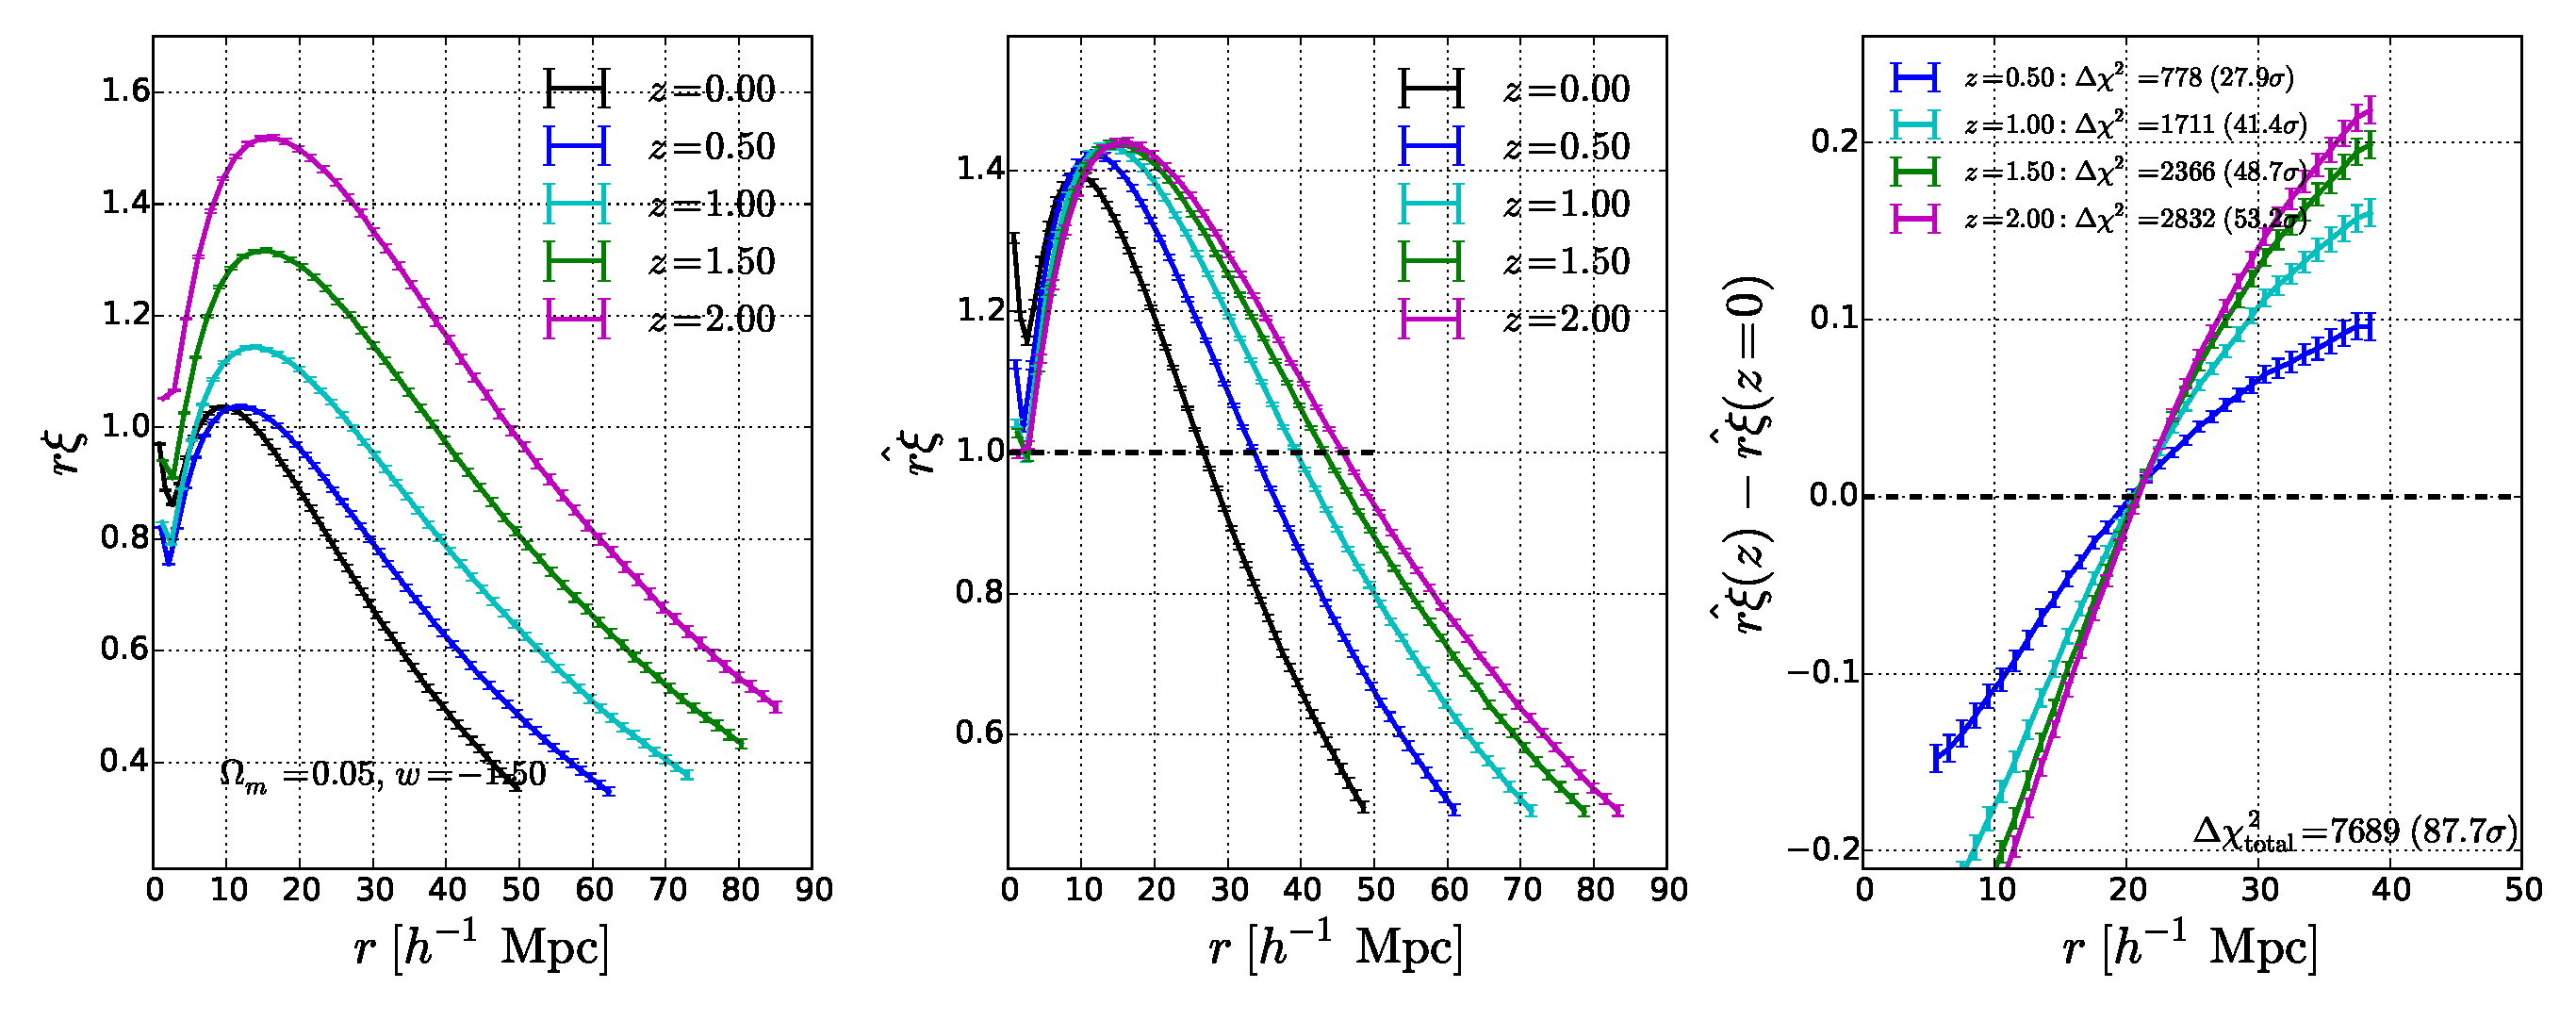
\includegraphics[width=18cm]{fig3_b.eps}
    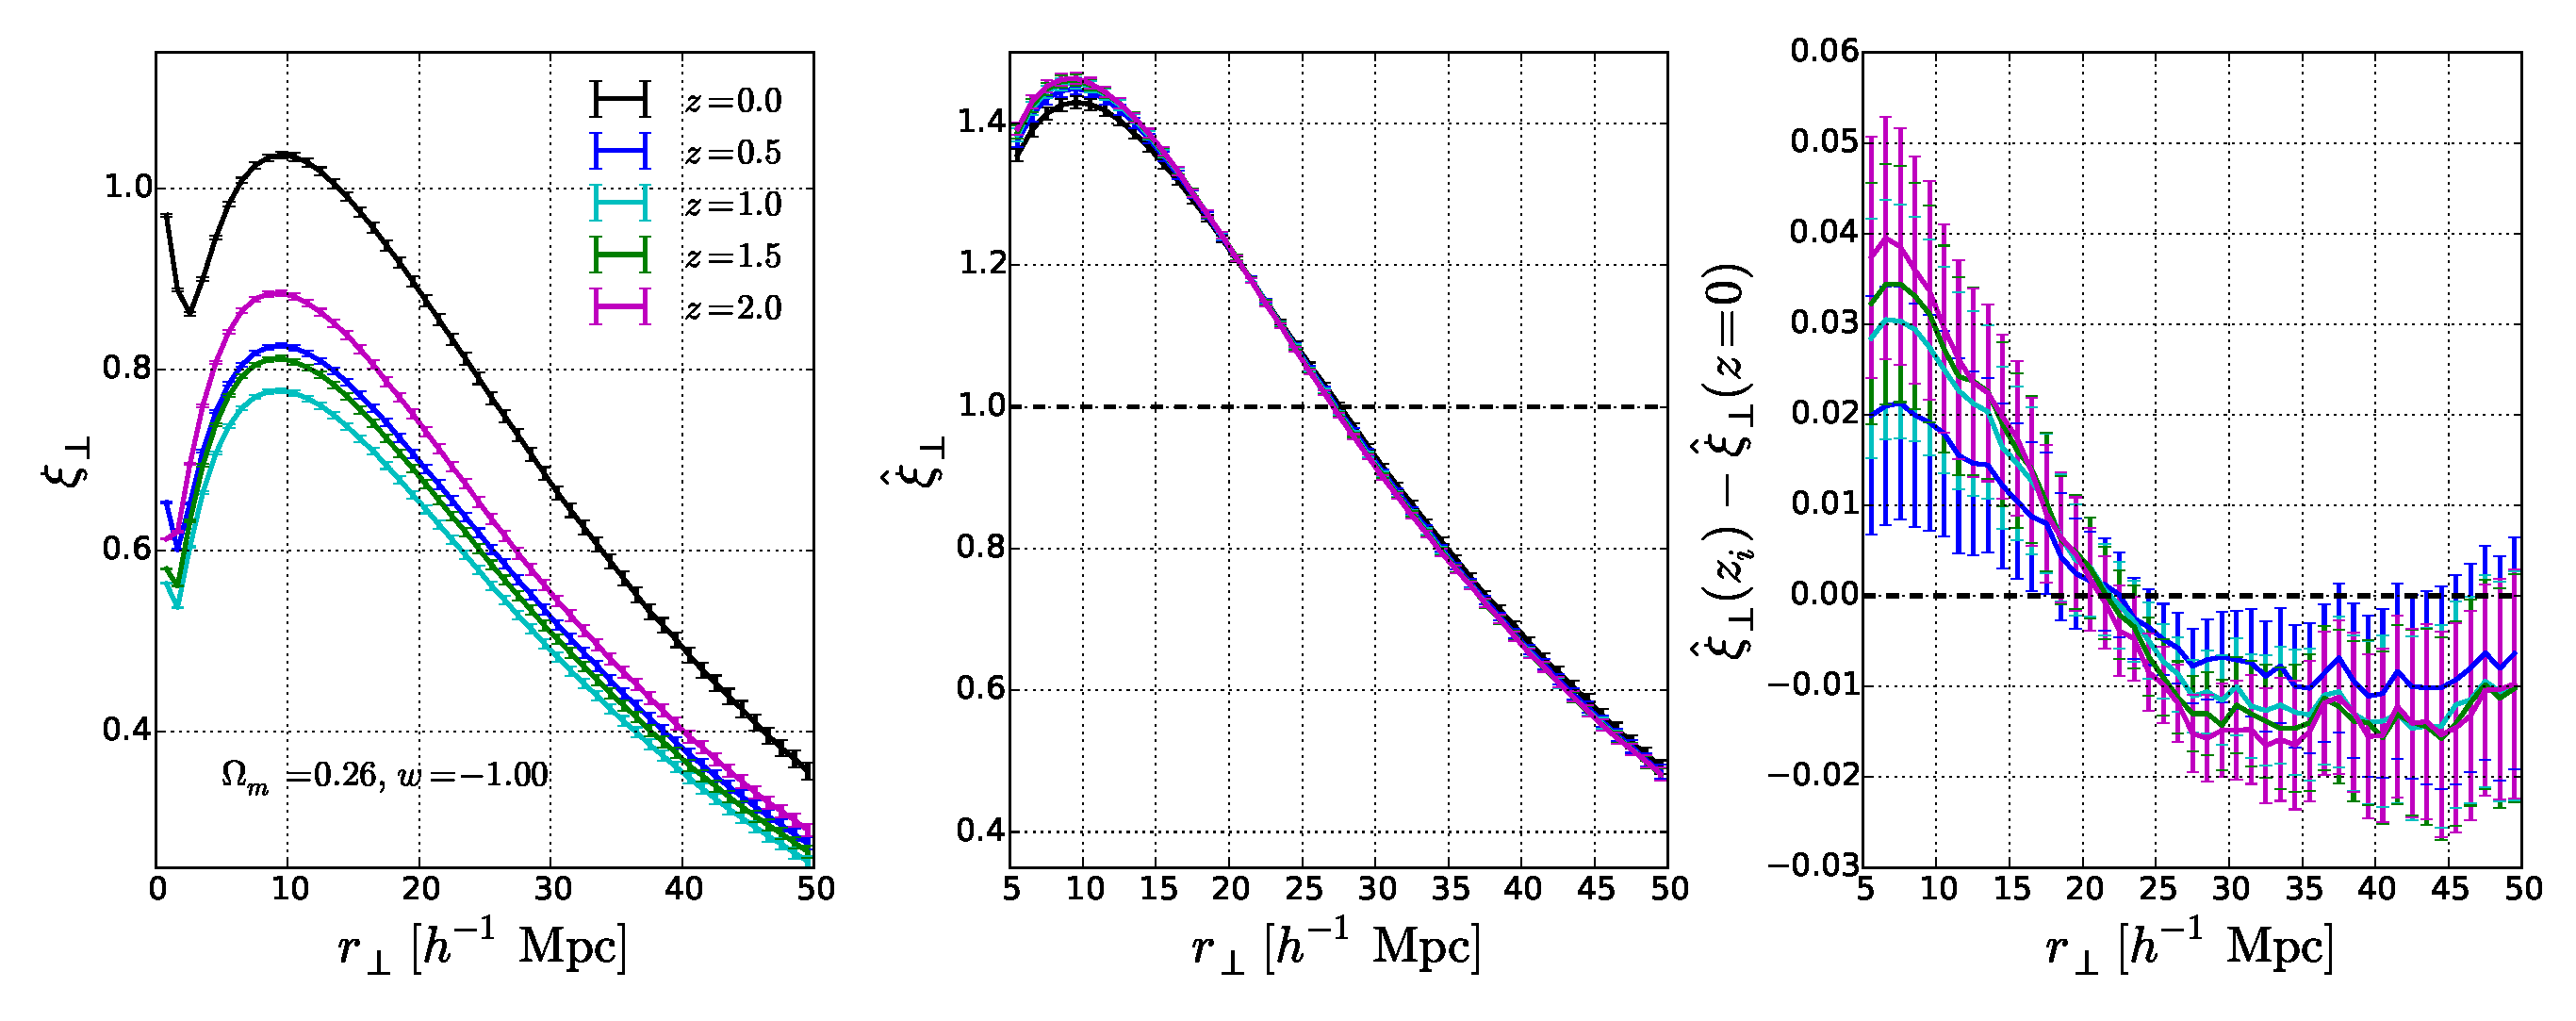
\includegraphics[width=2\columnwidth]{fig3.eps}
    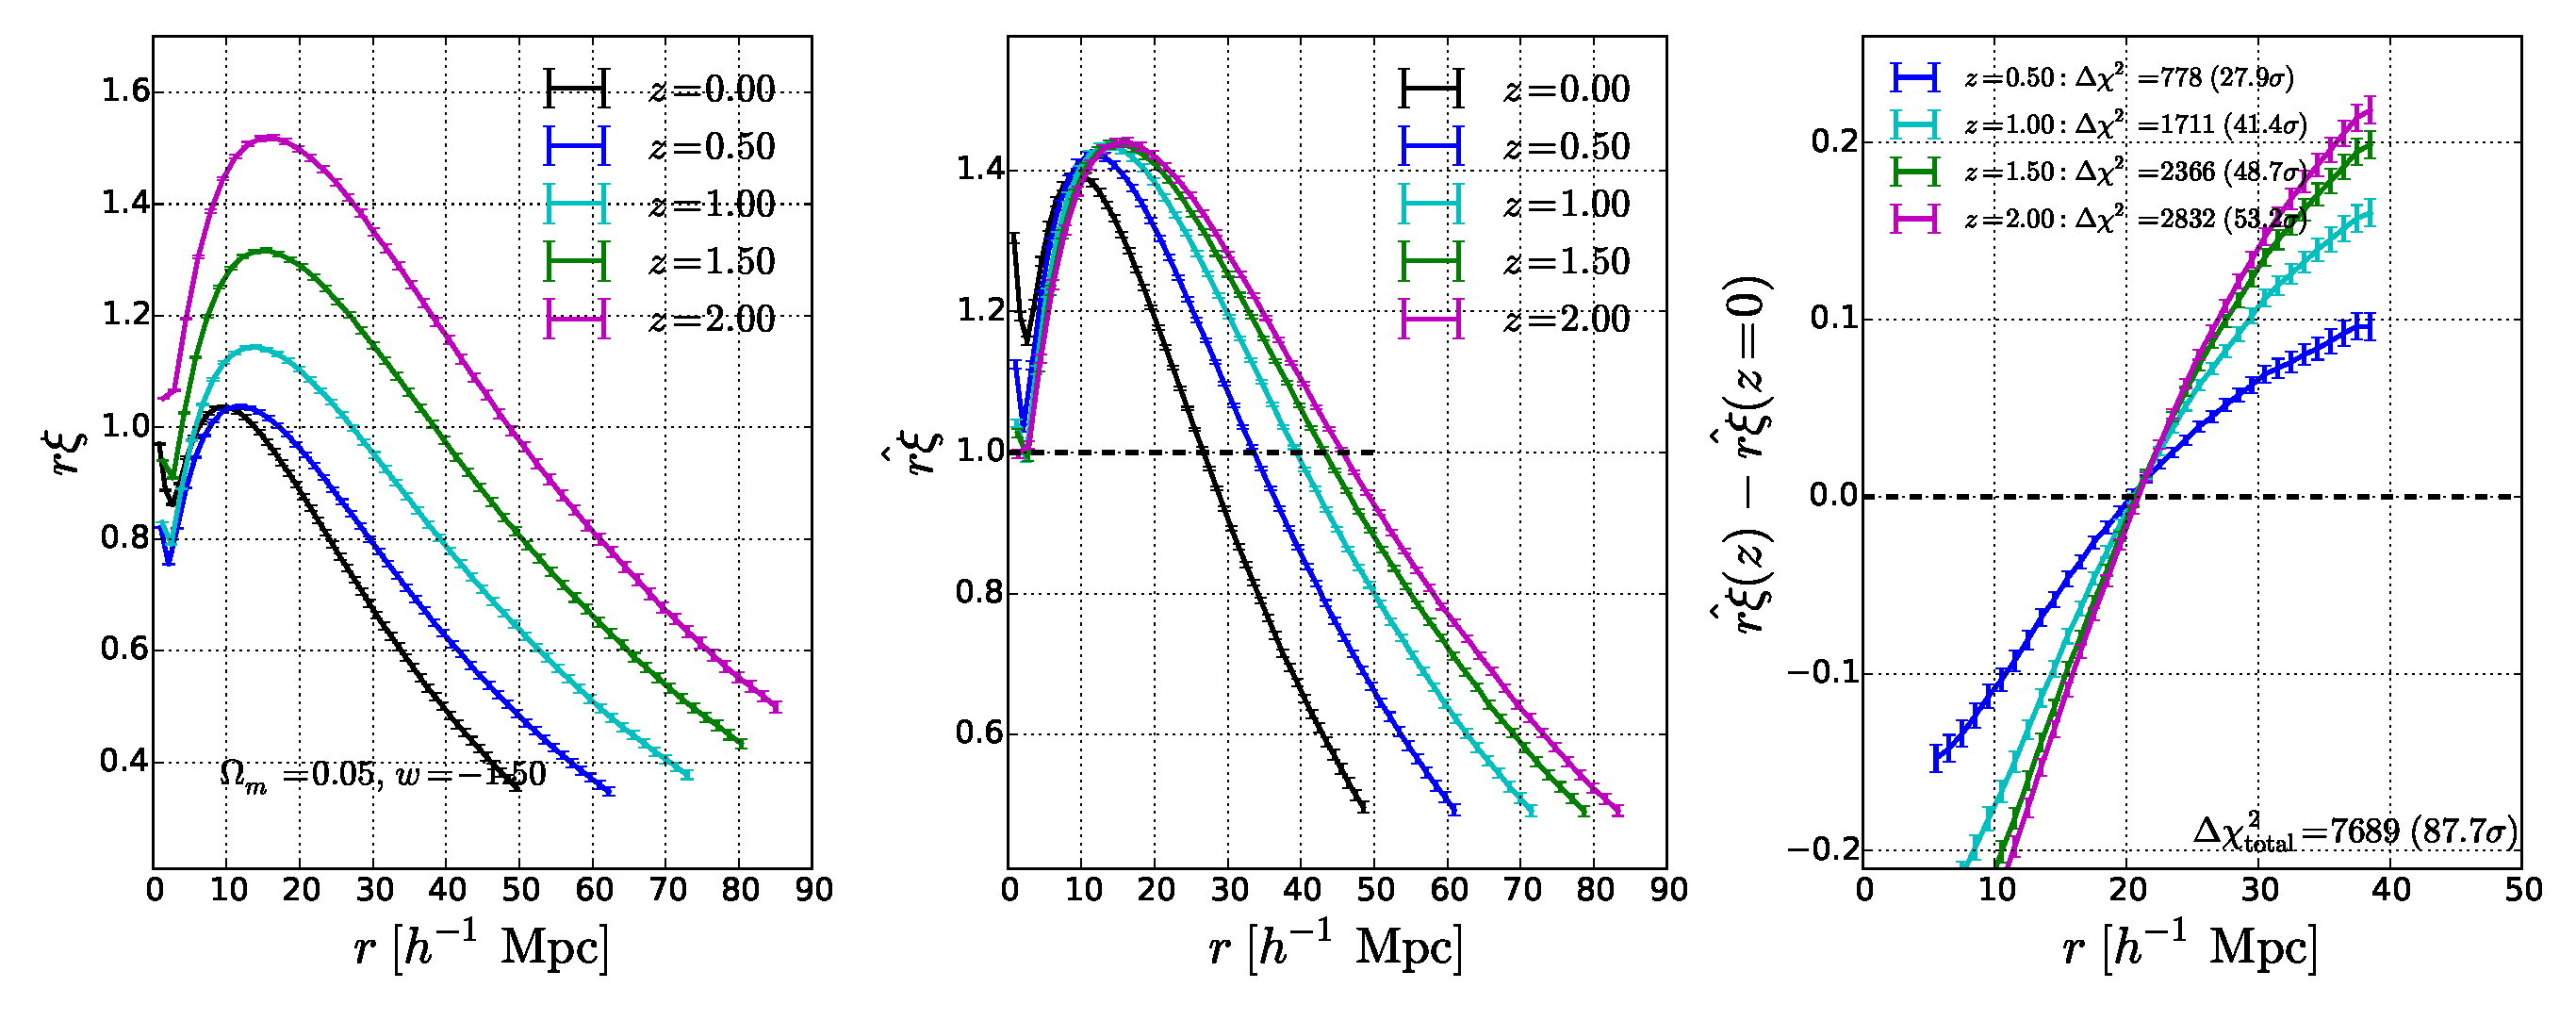
\includegraphics[width=2\columnwidth]{fig3_b.eps}
   }
   \caption{\label{fig_diffz}
  The 2pCF across the line-of-sight, $\xi_{r_\perp}$ (left panels), the shape of $\hat{\xi}_{r_\perp}$ (middle panels),
  and the evolution with respect to the $z=0$ value, $\hat{\xi}_{r_{\perp}}(z=z_i) - \hat{\xi}_{r_{\perp}}(z=0)$ (right panels). 
  Upper panels show that in the correct cosmology the redshift evolution of the shape of 2pCF is rather small regardless of the large redshfit evolution of the amplitude, 
  whereas the lower panels show that, in a wrong cosmology $\Omega_m = 0.05,w=-1.5$, the redshift evolution of $\hat{\xi}_{r_\perp}$ is very significant.
   }
\end{figure*}

The upper-left panel of Figure \ref{fig_diffz} displays the 2pCF across the line-of-sight measured from HR4 mock galaxies. % (multiplied by scale $r$) in the five snapshot.
We multiply $\xi$ by the separation $r_\perp$ to obtain a similar statistical uncertainty on all scales.
For convenience we will use the denotation
\begin{equation}
 \xi_{r_{\perp}} \equiv r_{\perp} \xi.
\end{equation}


Among the different redshift bins there is large variation in the amplitude of $\xi(r_\perp)$.
The amplitude is proportional to the clustering strength, which is affected by the gravitational growth of structures and the galaxy bias.
The amplitude is highest at $z=0$ where the structures experienced the most growth.
$\xi(r_\perp)$ increases at $z>1$ with increasing redshift 
due to the increasing galaxy bias.
%leading to stronger clustering strength and higher amplitude of 2pCF.
%On the contrary, at higher redshift we find $\xi(z=2)>\xi(z=1.5)>\xi(z=1)$,
%The trend is different from $z=1,1.5,2$,
%simply because by applying a uniform mass cut we are selecting more biased galaxies at higher redshift.

Although there is large variation in amplitude between the different redshifts bins, 
%The shape of $r_\perp\xi$ also evolves with redshift.
the shape of $\xi_{r_{\perp}}$  remains similar at all redshifts;
in general it peaks at $r\sim9 h^{-1}\rm Mpc$ and monotonically drops or increases at larger or smaller scales.
The only exception is the small enhancement at $r\lesssim 2 h^{-1}\rm Mpc$,
which is caused by the non-linear growth of structures 
and is much more significant at lower redshift.

In order to directly compare the shape of the 2pCF at different redshifts,
in the middle panel of Figure \ref{fig_diffz} 
we show the $r_\perp\xi$ normalized by the overall amplitude within 
$5h^{-1}{\rm Mpc} < r < 40h^{-1}{\rm Mpc}$
(here after $\hat \xi_{r_\perp}$):
\begin{equation}
 \hat \xi_{ r_\perp} \equiv  \frac{ {r_\perp\xi}(r_{\perp})}{ \int_{r_{\perp, \rm min}}^{r_{\perp, \rm max}}r_{\perp} \xi(r_{\perp}) d r_{\perp} / (r_{\perp,\rm max}-r_{\perp,\rm min}) },
\end{equation}
where we choose $r_{\perp, \rm min}=5 h^{-1}$ Mpc, $r_{\perp, \rm max}=40 h^{-1}$ Mpc in this analysis.
Below $5 h^{-1}$ Mpc the non-linear growth of structure 
leads to systematic redshift evolution which could be difficult to be reliably accounted;
On scales larger than $40 h^{-1}$ Mpc,
the analytical modeling of the shape of $\xi_{r_{\perp}}$ is relatively well understood;
one can just fit the 2pCF with the theoretical predictions \citep{BCGS2001,Salvador2014,Salvador2016} 
instead of using our method 
(although our method should also be applicable).

In the upper-middle panel, the overlapping of $\hat\xi_{r_{\perp}}$
clearly show the minimal redshift evolution of the shape.
In the upper-right panel, 
we further show the residual evolution at high redshifts 
with respect to $z=0$.
There is only 1-4\% enhancement 
at $r<10h^{-1}\rm Mpc$,
and $<1.5\%$ suppression at $r>25 h^{-1}\rm Mpc$.
The trend is monotonic with redshift.

There is one detail in the analysis that should be emphasized here.
In real observations we may be selecting {\it different} types of galaxies at different redshifts.
Considering this fact in the comparison of $\hat\xi_{r_\perp}$ 
we compare subsamples of galaxies at {\it different} locations.
As an example, if at $z=0$ we take $\hat\xi_{r_\perp}$ measured within $0h^{-1}{\rm Mpc}<Z<105 h^{-1}{\rm Mpc}$,
at higher redshifts we then adopt measurement within $105h^{-1}{\rm Mpc}<Z<210 h^{-1}{\rm Mpc}$ for a comparison.
%and take the difference between them to get $\delta \hat{r_\perp\xi}$.
%So we are always comparing 2pCF measured from different samples of galaxies.
If we simply compare the 2pCF of the {\it same} subsample of galaxies at different redshifts, 
one would significantly underestimate the statistical uncertainty of $\delta \hat{\xi}_{r_\perp}$ by ignoring cosmic variance.
%The error bars and covariance are always estimated in this way to take the cosmic variance into consideration.
%\footnote{In all figures of this paper The error bars displayed in all figures are estimated in this way; 
%from the 120 subsamples and for the error bar of redshift evolution of 2pCF 
%we always take the cosmic variance into consideration.}.


%As shown by Figure \ref{fig_scatter}, the gravitational growth of strucutre enhance the clustering strengh of structures on all scales;
%here it manifests itself as an enhanced amplitude of 2pCF at low redshift.
%The shape of 2pCF, which represents the {\it relative strength of clustering among different scales},
%maintain similar with redshift except the non-linear scales of $r_\perp < 5 h^{-1}\rm Mpc$.
%mainly increases the amplitude of 

%In all, we conclude that the shape of the 2pCF is more robust than the amplitude against redshift and galaxy bias.

\subsection{Galaxy 2pCF across the line-of-sight: cosmological effect }

The 2pCF across the line-of-sight for galaxy positions constructed in a wrongly assumed cosmology $\Omega_m=0.05,\ w=-1.5$
is displayed in the lower panels of Figure \ref{fig_diffz}.
The mis-scaling uniformly shifts the clustering pattern on all scales, 
leading to a biased $\hat \xi_{r_\perp}$, which is 
related with the true $\hat \xi$ as
\begin{equation}
 \hat \xi_{r_\perp,\rm wrong}(r) = \hat \xi_{r_\perp, \rm correct}(\alpha_{\perp} r),
\end{equation}
a simple consequence of the fact that the clustering pattern at scale $r$ is rescaled to $\alpha_{\perp} r$.

The redshift evolution of $\alpha_{\perp}$ leads to redshift evolution of 
$\hat \xi_{r_\perp, \rm correct}$,
%Lower panels of Figure \ref{fig_diffz} shows the $r_\perp\xi$ in five 
%snapshots, in case that the cosmology $\Omega_m=0.05,\ w=-1.5$ 
%is adopted to construct the galaxy distribution (the right panels of Figure \ref{fig_scatter}).
which is displayed in the lower-middle panel.
The upscaling of comoving distance leads to a stretched shape.
When increasing redshift,
the peak location is shifted from $\sim9h^{-1} \rm Mpc$ to $\sim15 h^{-1}\rm Mpc$ at $z=2$,
as a result of the fact that the $\hat\xi_{r_{\perp}}$ separation is upscaled by $71.7\%$.
Correspondingly, the right panel shows that, 
compared with $\hat \xi_{r_\perp}$ at $z=0$ there is a 20-40\% change at higher redshifts.

The mis-scaling not only changes the shape of the 2pCF but also changes the value of $ \xi_{r_\perp}$. %The amplitude of $r_\perp\xi$ is amplified due to the stretch of scale.
As is shown in the left panel, due to the stretch of scale the amplitude is enhanced at higher redshifts;
the higher the redshift, the greater the enhancement
\footnote{The value of $\xi$ is not affected by the mis-scaling. 
But since we are using $r_\perp\xi$ rather than $\xi$, the y-axis values are affected. 
For a 20\% up-rescaling, the peak value of $r_\perp\xi$ is also increased by 20\%.}.%the amplitude monotonically increases as a function of redshift.

Although the change of amplitude could be a more significant cosmological consequence 
than the alteration of shape,
it is mixed with the other effects; i.e.
the growth of structure and a larger galaxy bias can also lead to a stronger clustering and thus an enhanced amplitude.
%it is more difficult to 
%But this phenomenon can also appear in case of gravitational growth of structure or increasing of bias,
%so we will not make use of it to do cosmological constraint.
In order to reliably extract the cosmological information, 
we just utilize the redshift evolution of the 2pCF shape, 
which is less affected by these complicated factors.
%which is as a signal suggesting that the assumed cosmological parameters are wrong.


\subsection{Systematic effects}

\begin{figure*}
   \centering{
   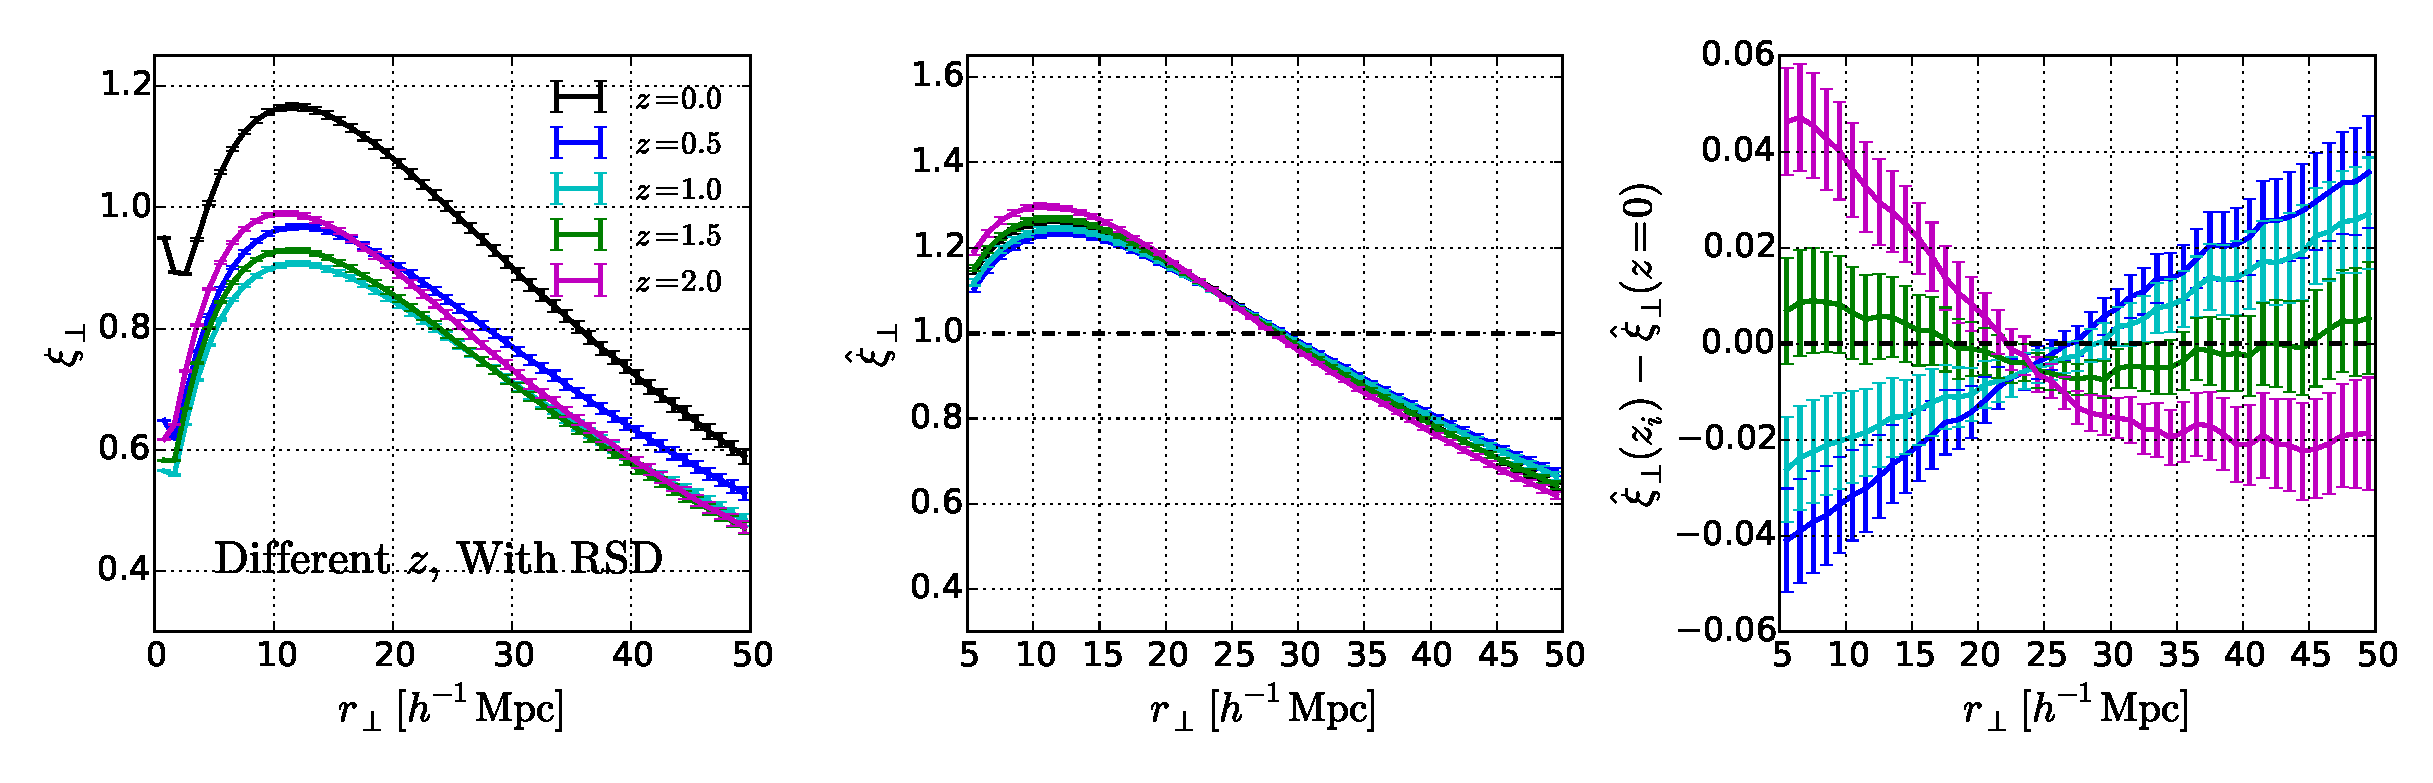
\includegraphics[width=2\columnwidth]{fig4_a.eps}
   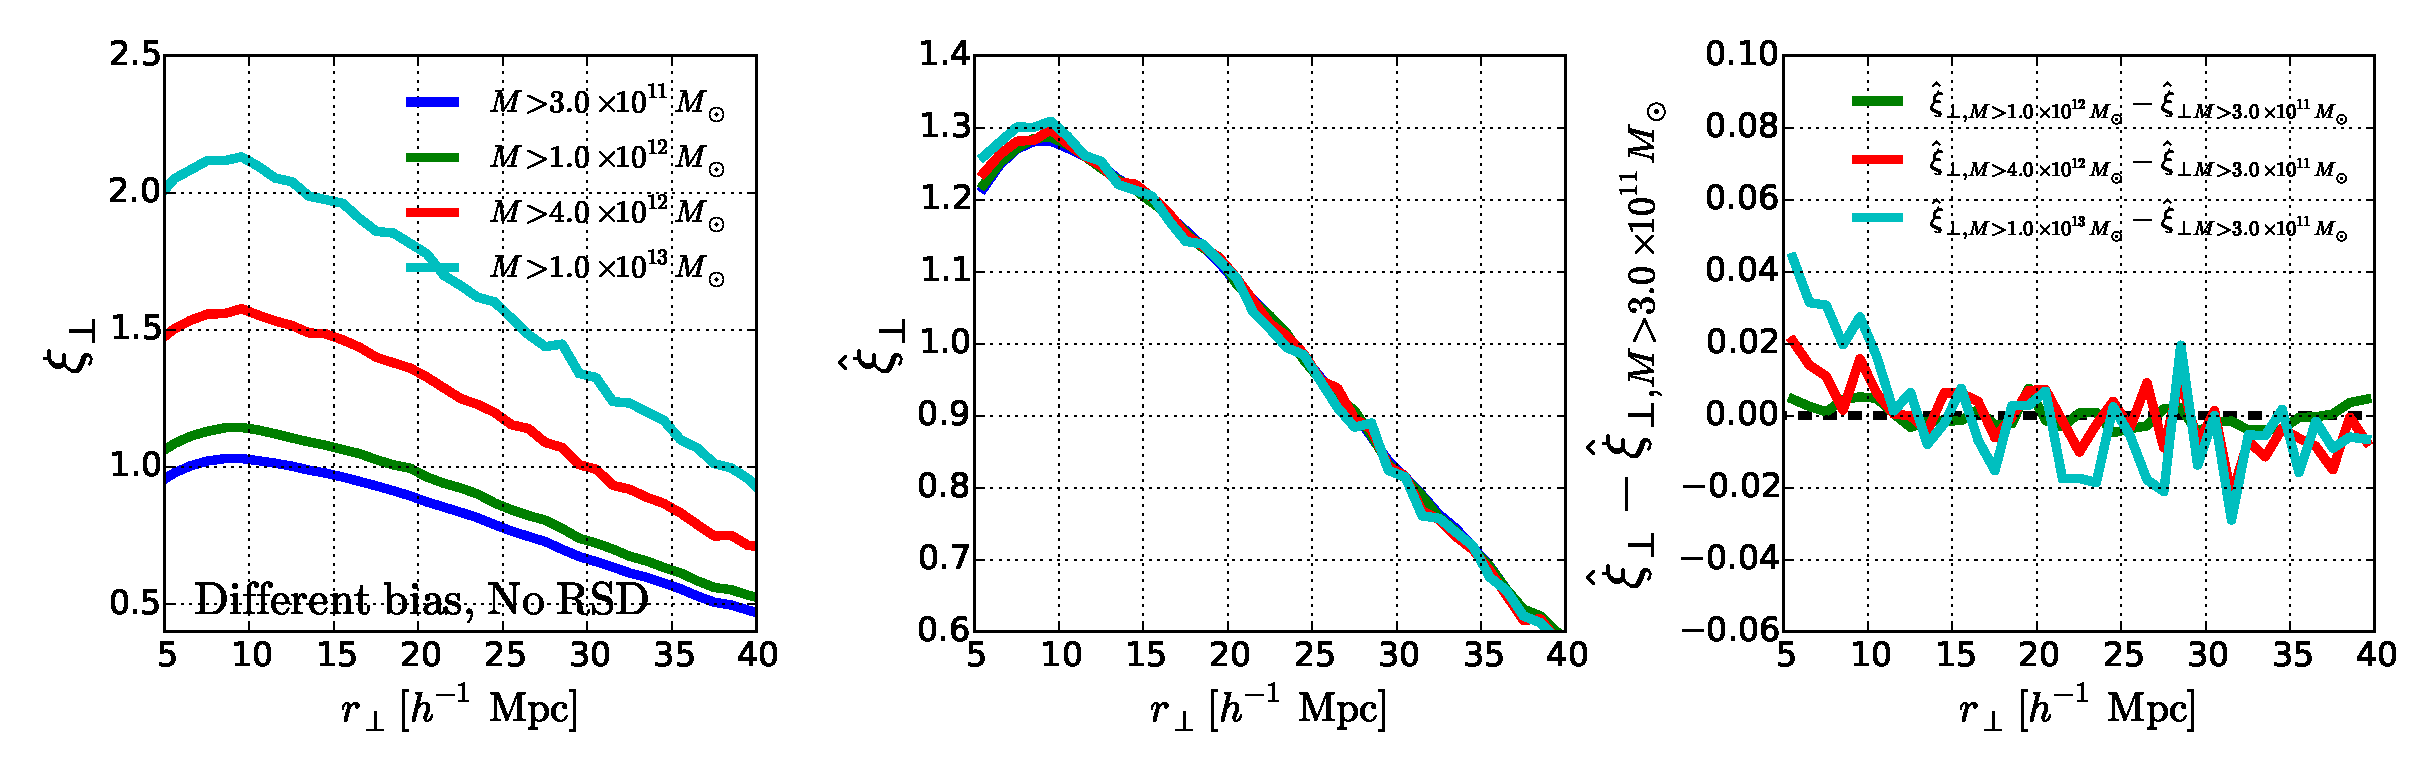
\includegraphics[width=2\columnwidth]{fig4_b.eps}
   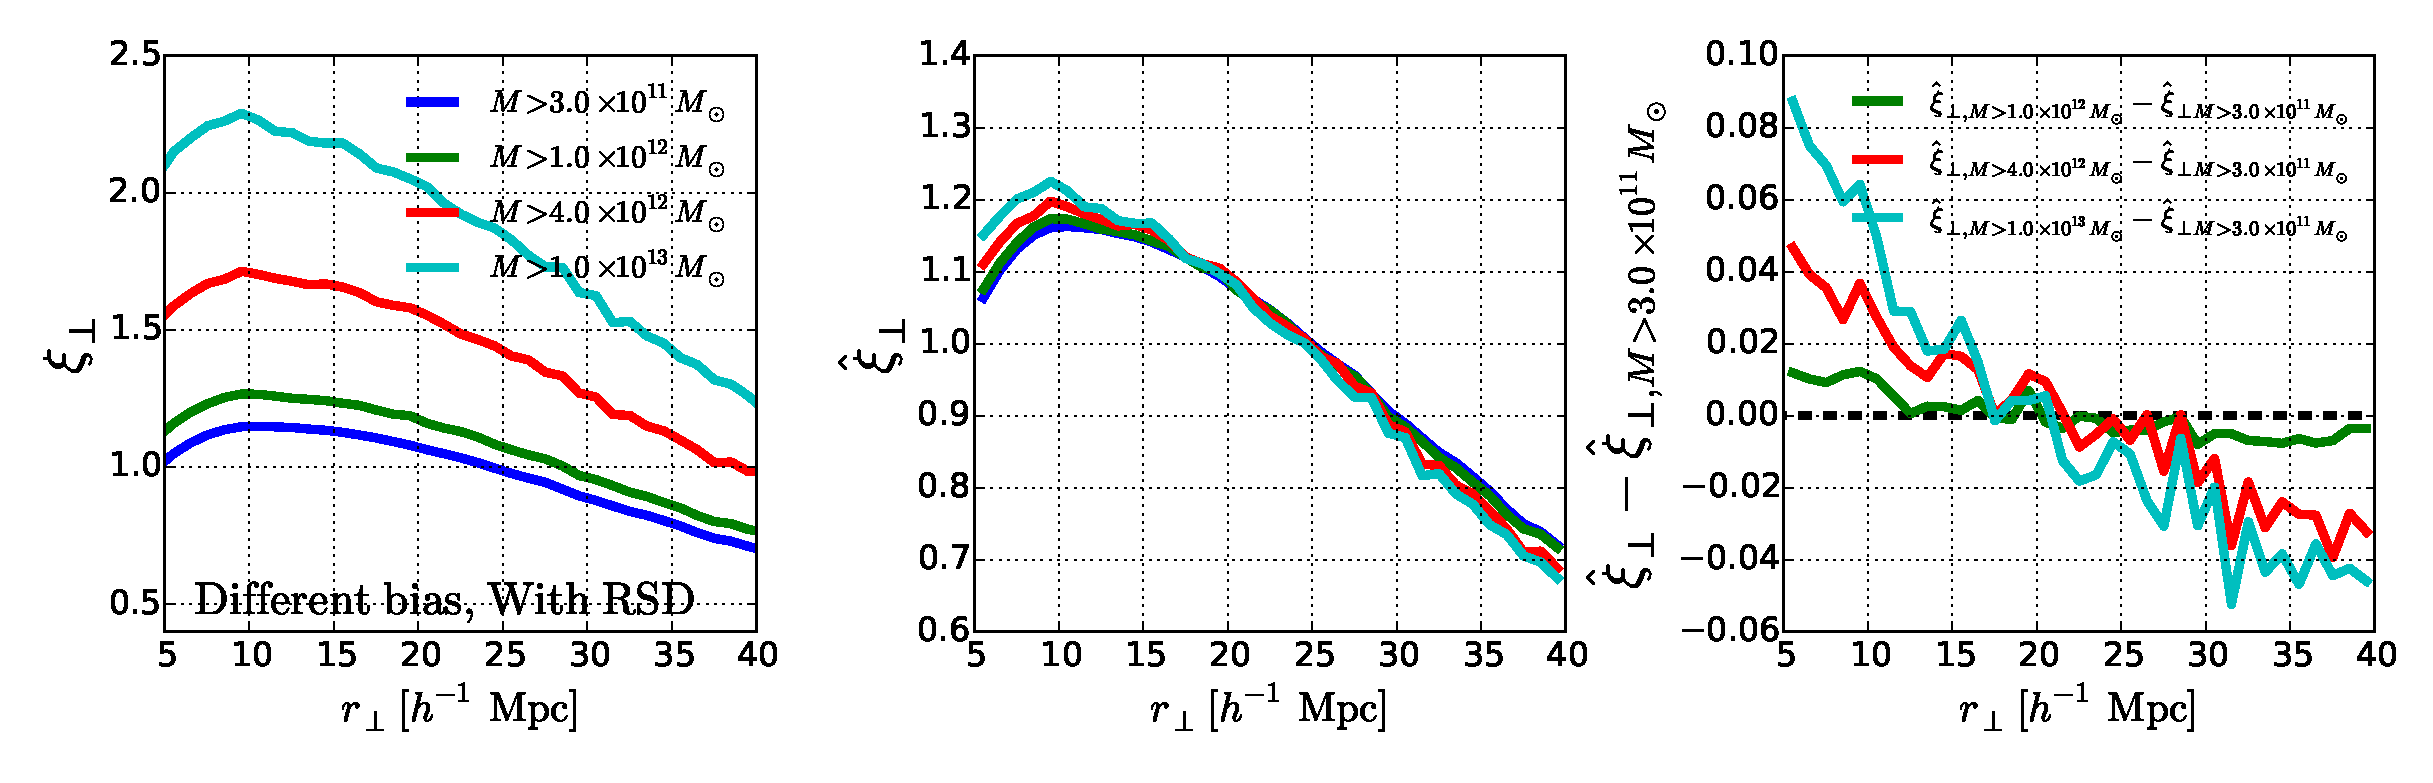
\includegraphics[width=2\columnwidth]{fig4_c.eps}
   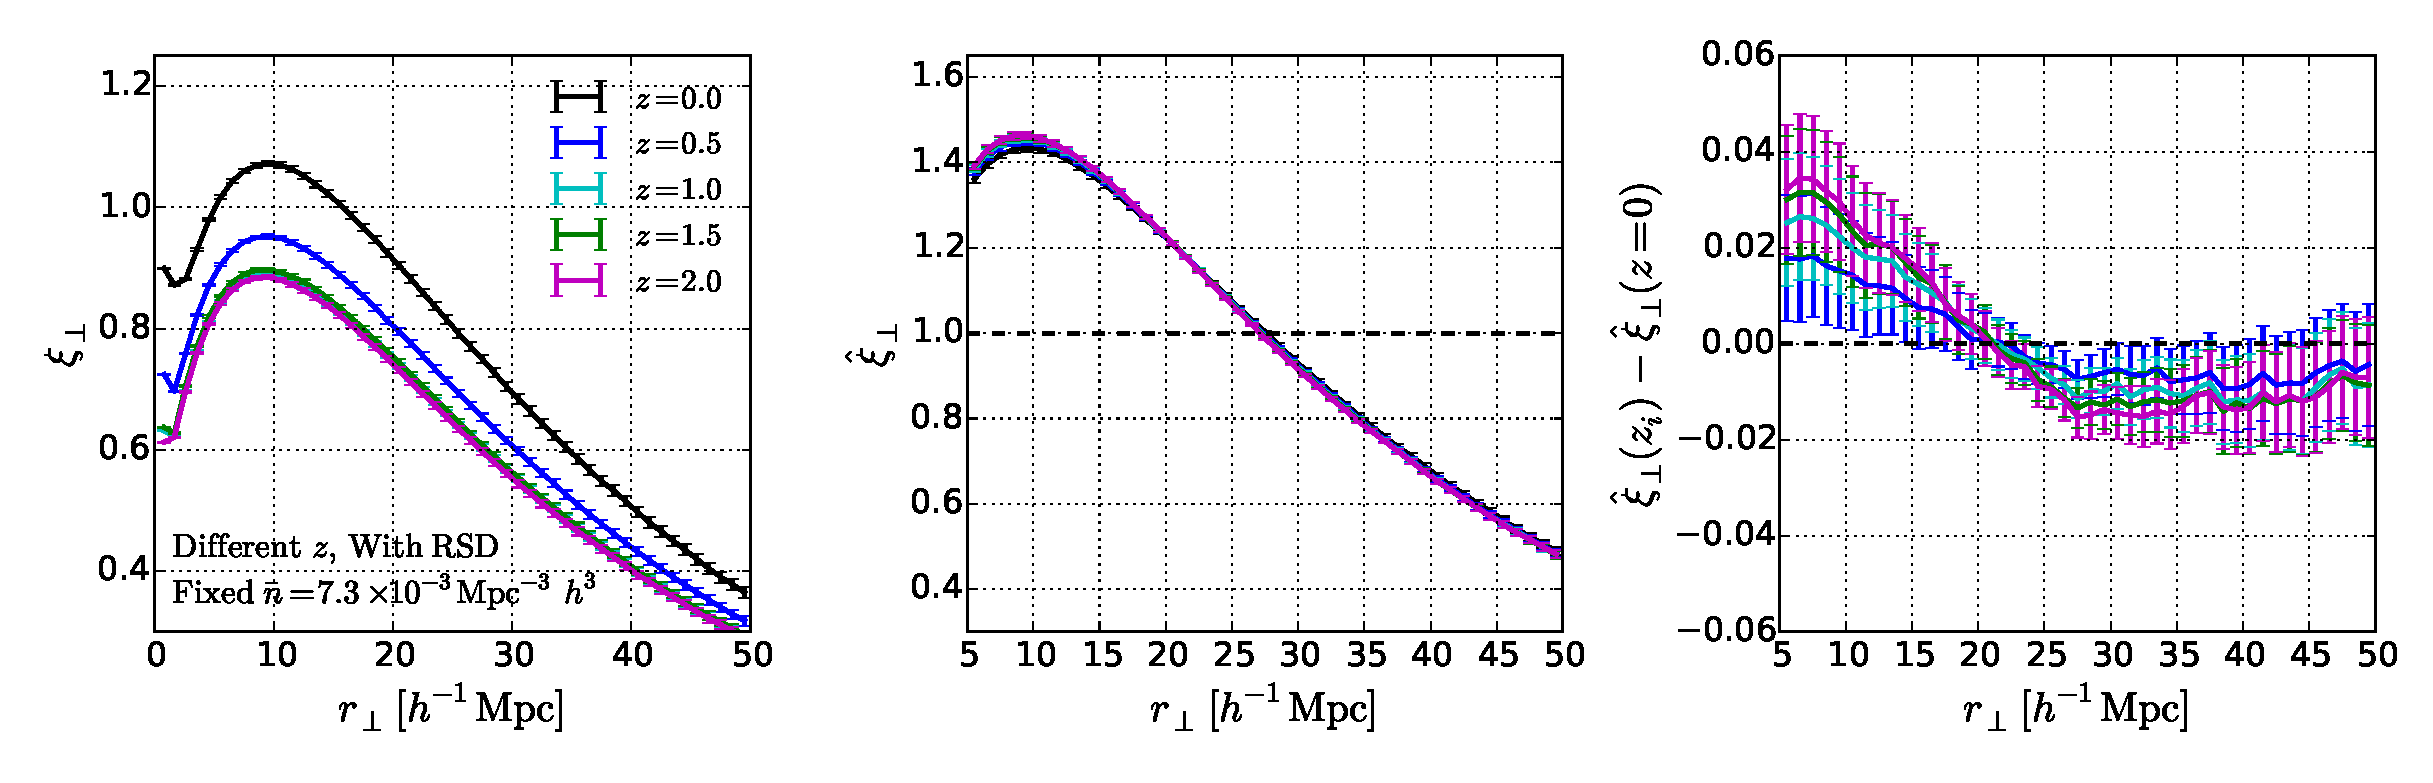
\includegraphics[width=2\columnwidth]{fig4_d.eps}
   }
   \caption{\label{fig_sys}
  First row: $\xi_{r_\perp}$ (left), $\hat{\xi}_{r_\perp}$ (middle), and $\hat\xi_{r_\perp}(z=z_i)-\hat\xi_{r_\perp}(z=0)$ (right) calculated with the RSD effect included.
  Second row: $\xi_{r_\perp}$ (left) and $\hat{\xi}_{r_\perp}$ (middle) are shown for four different halo-mass-cuts, $3\times 10^{11},~1\times 10^{12},~4\times 10^{12},~\&~1\times 10^{13}~M_\odot$, 
  below which we remove from 2pCF calculation. 
  The right panel shows the difference in $\hat{\xi}_{r_\perp}$ between the $3\times 10^{11}~M_\odot$ mass-cut case and the other mass-cut cases. 
  Third row: The same as the second row panels, except that the RSD effect is considered.
  Fourth row: The redshift evolution in case of using {\it samples with constant number density} $\bar n=7.3\times 10^{-3} {\rm Mpc}^{-3}h^3$, 
  and the RSD effect is considered. } 
\end{figure*}



In Sec. \ref{sec_2pCF_diffz} we showed that $\hat \xi_{r_\perp}$ measured from the
constant mass cut samples at different redshifts show good agreement.
The gravitational growth of structure will not have a large impact on $\hat \xi_{r_\perp}$ on scales $\gtrsim5 h^{-1}$ Mpc,
yet there are many other factors that may induce redshift evolution
including galaxy bias, RSD, redshift error, and 
the redshift evolution of galaxies properties 
such as mass, morphology, color, concentration. 
Here we test two ``major'' systematical effects;  the RSD effect and galaxy bias.

%The same as \cite{Li2014,Li2015,Li2016} we need to correct for the redshift evolution of $r_\perp\xi$ caused by effects other than the cosmological effect.

%Figure \ref{fig_diffz} already shows that, the growth of structure, especially in low redshift and on non-linear scales, 
%changes the shape of $r_\perp\xi$ and caused relative enhancement on $r\lesssim2 h^{-1}\rm Mpc$.
%So we limit the region of scale to $r>5h^{-1}\rm Mpc$ to minimize its effect.

\subsubsection{Redshift Space Distortion}


\begin{figure*}
   \centering{
%   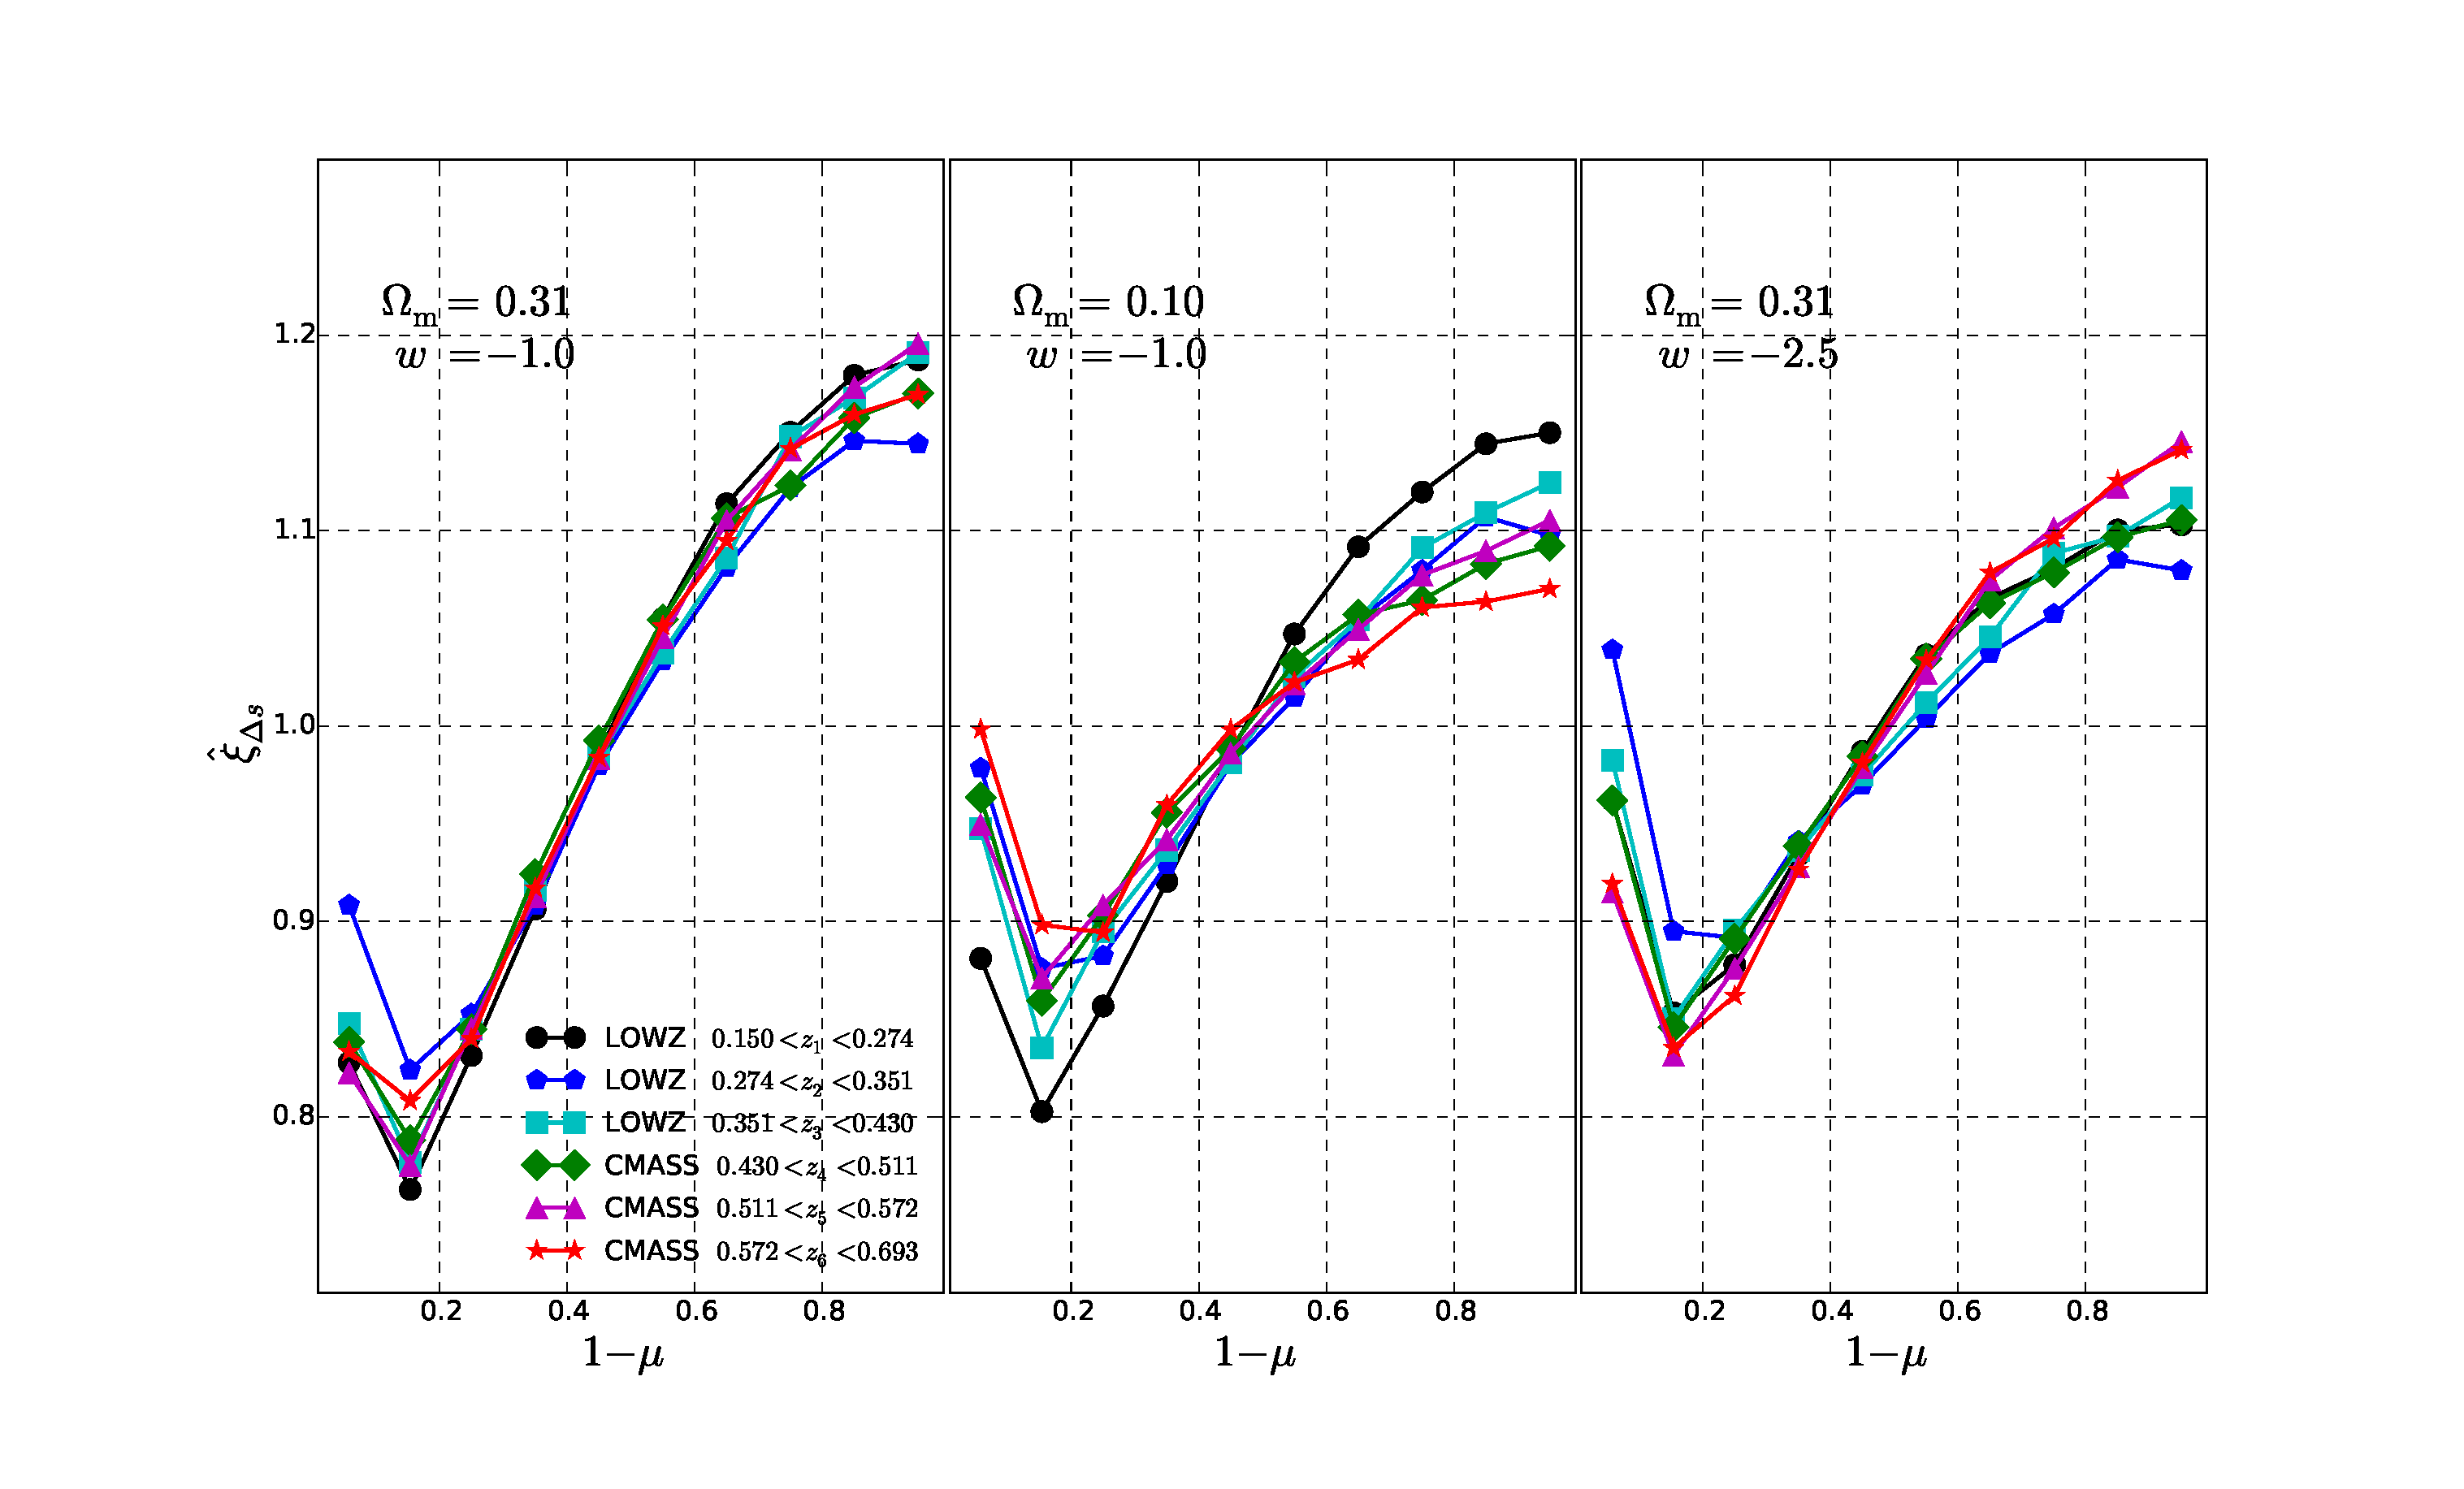
\includegraphics[width=18cm]{fig9_0.eps}
%   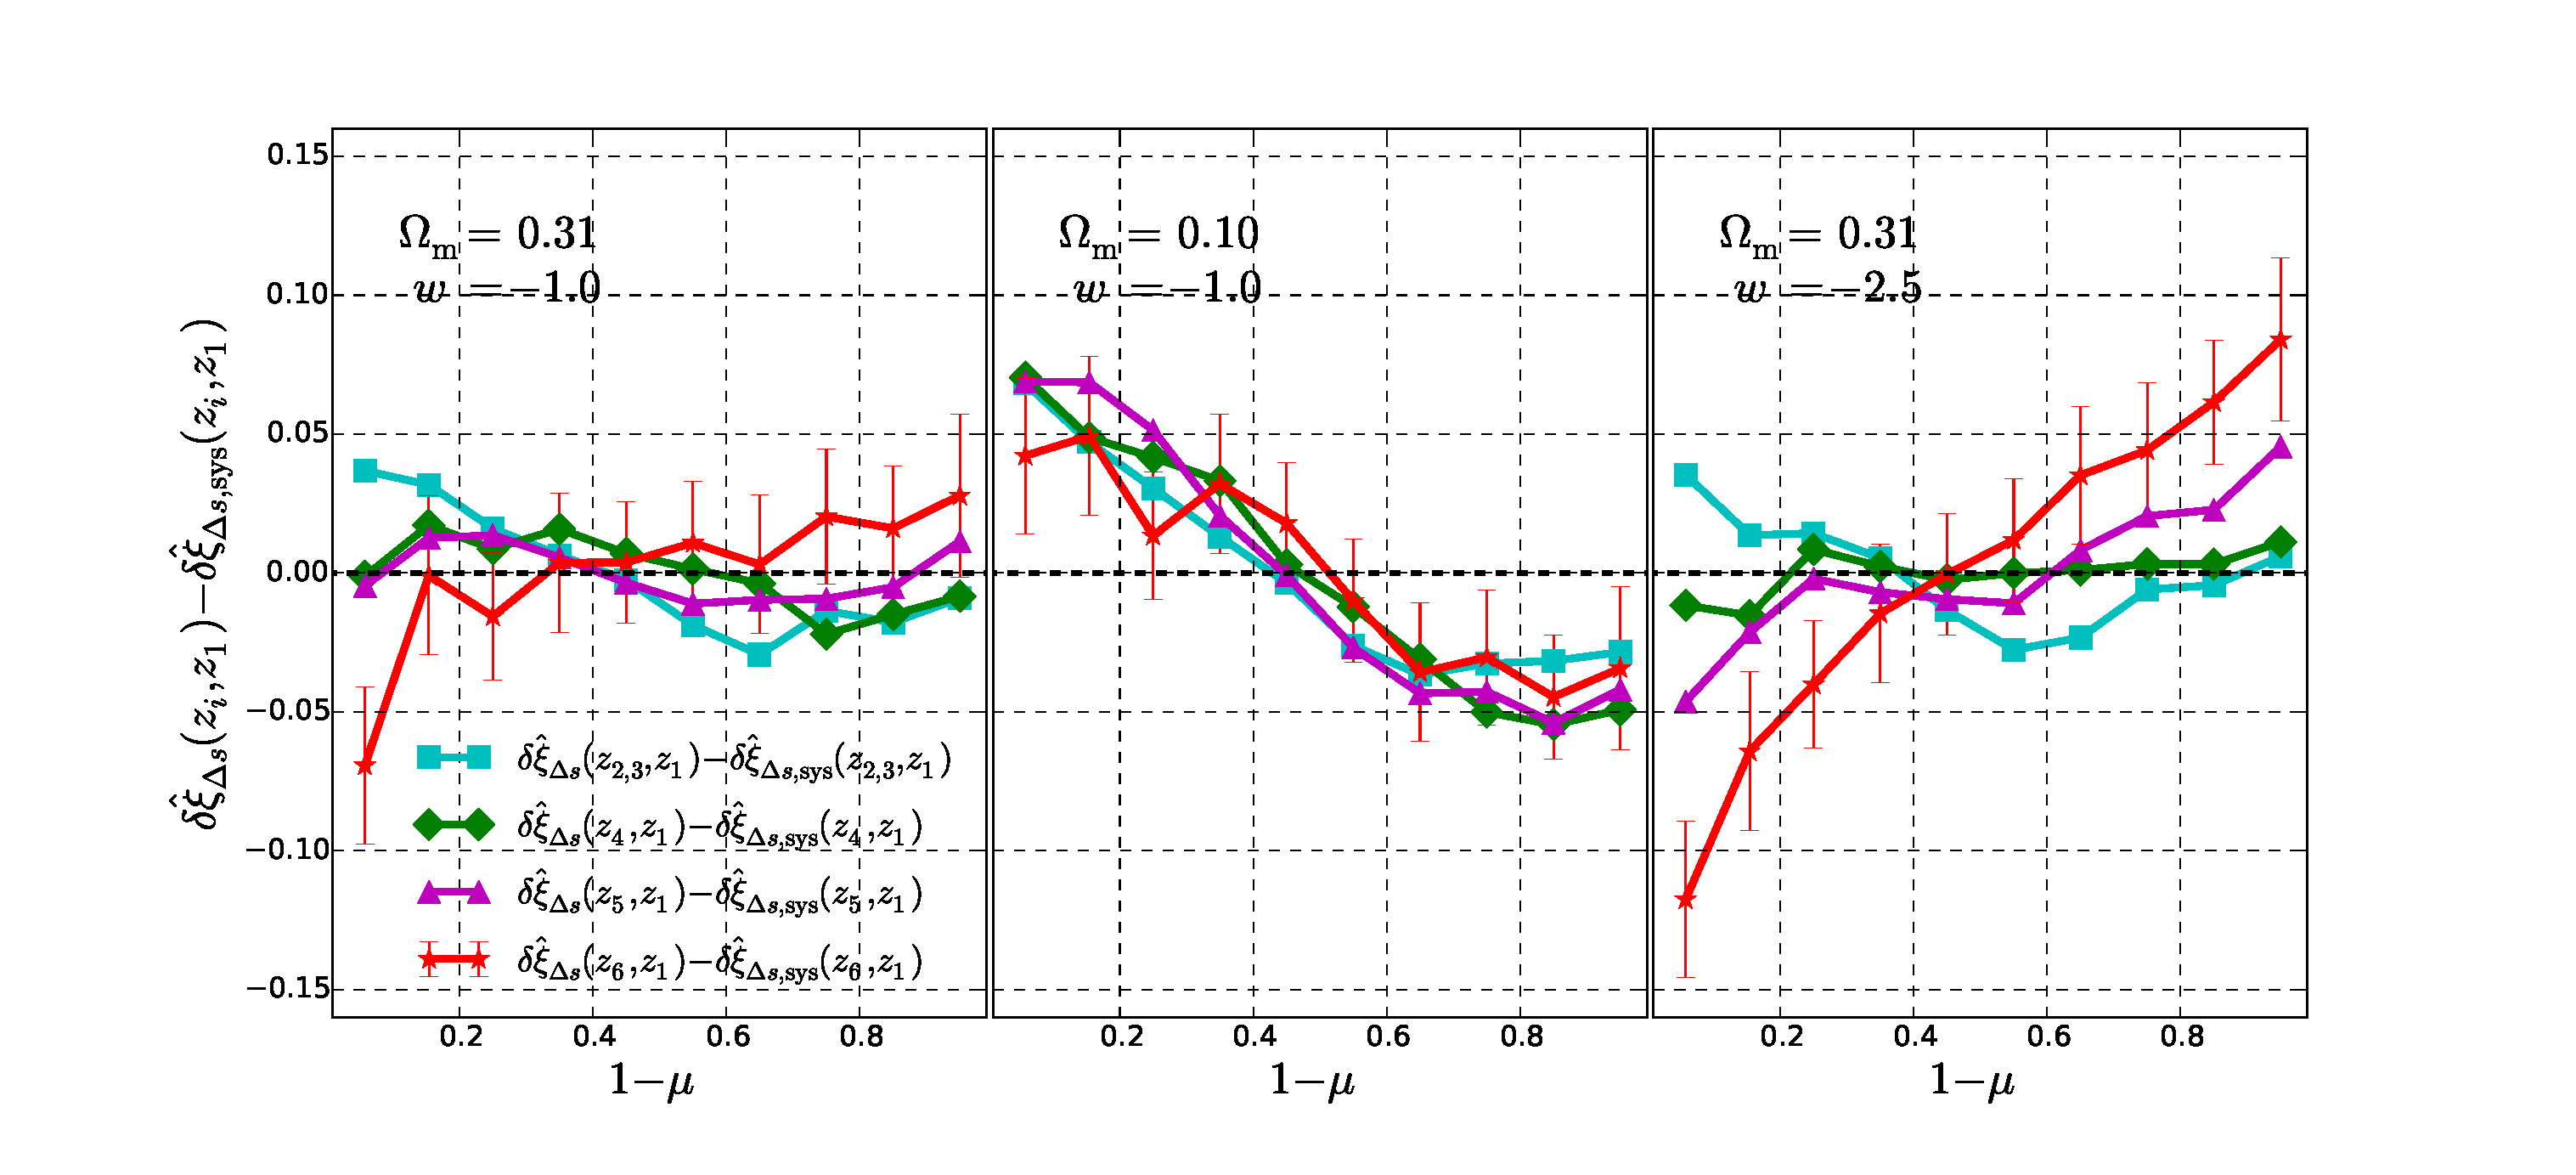
\includegraphics[width=18cm]{fig9_1.eps}
%   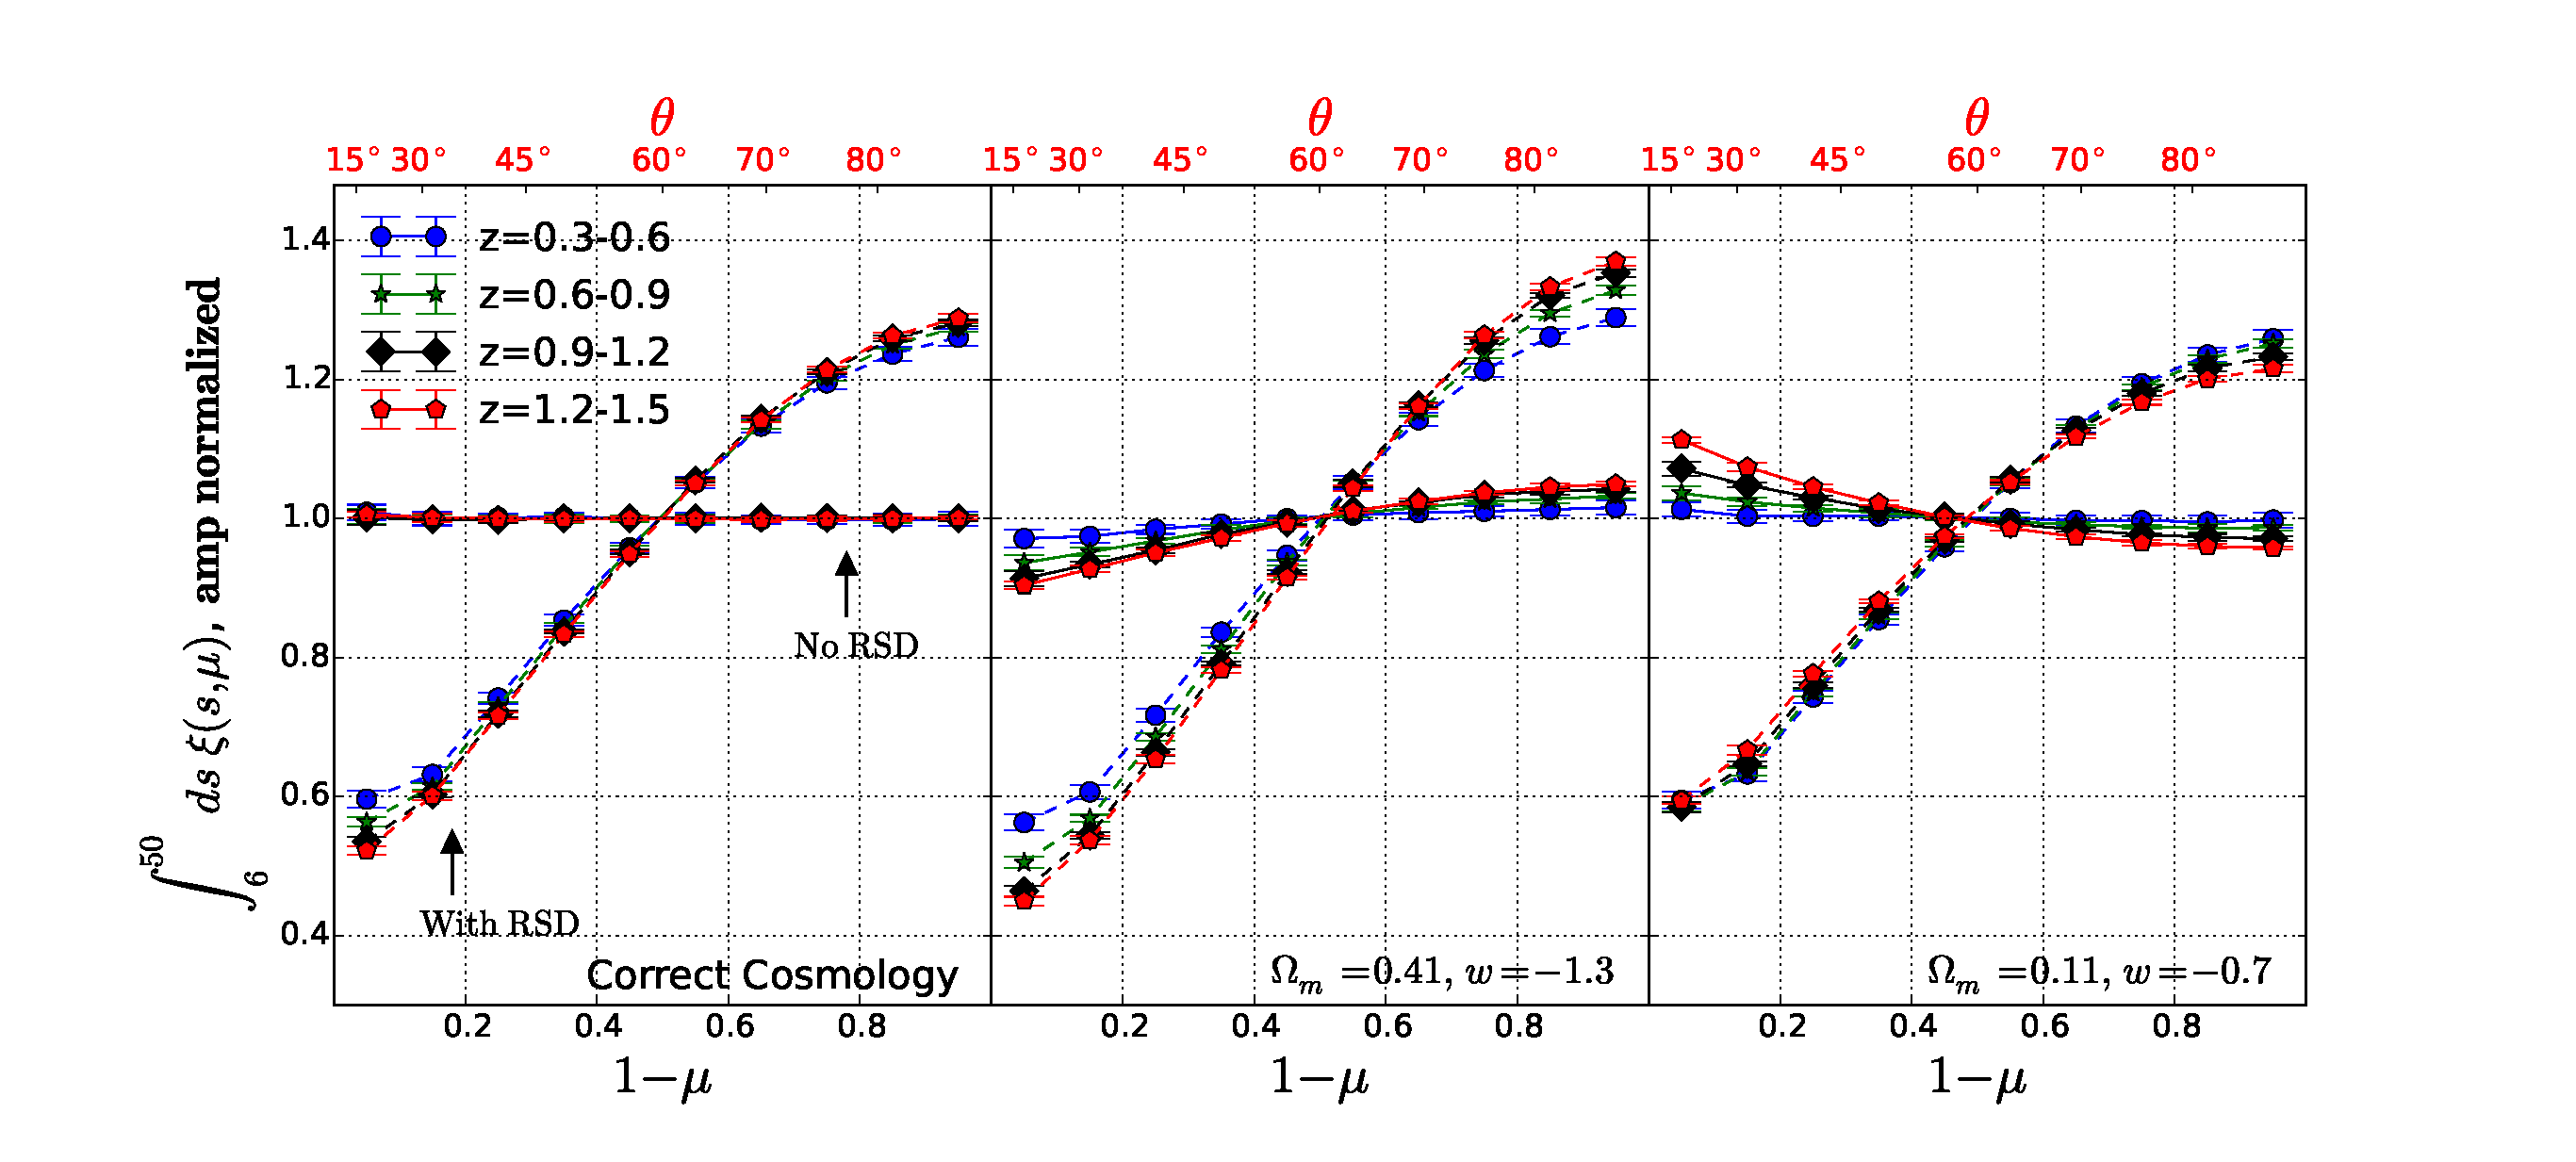
\includegraphics[height=8cm]{Tpcf--plot--Normed.eps}
%    \includegraphics[height=8cm]{smu.eps}
    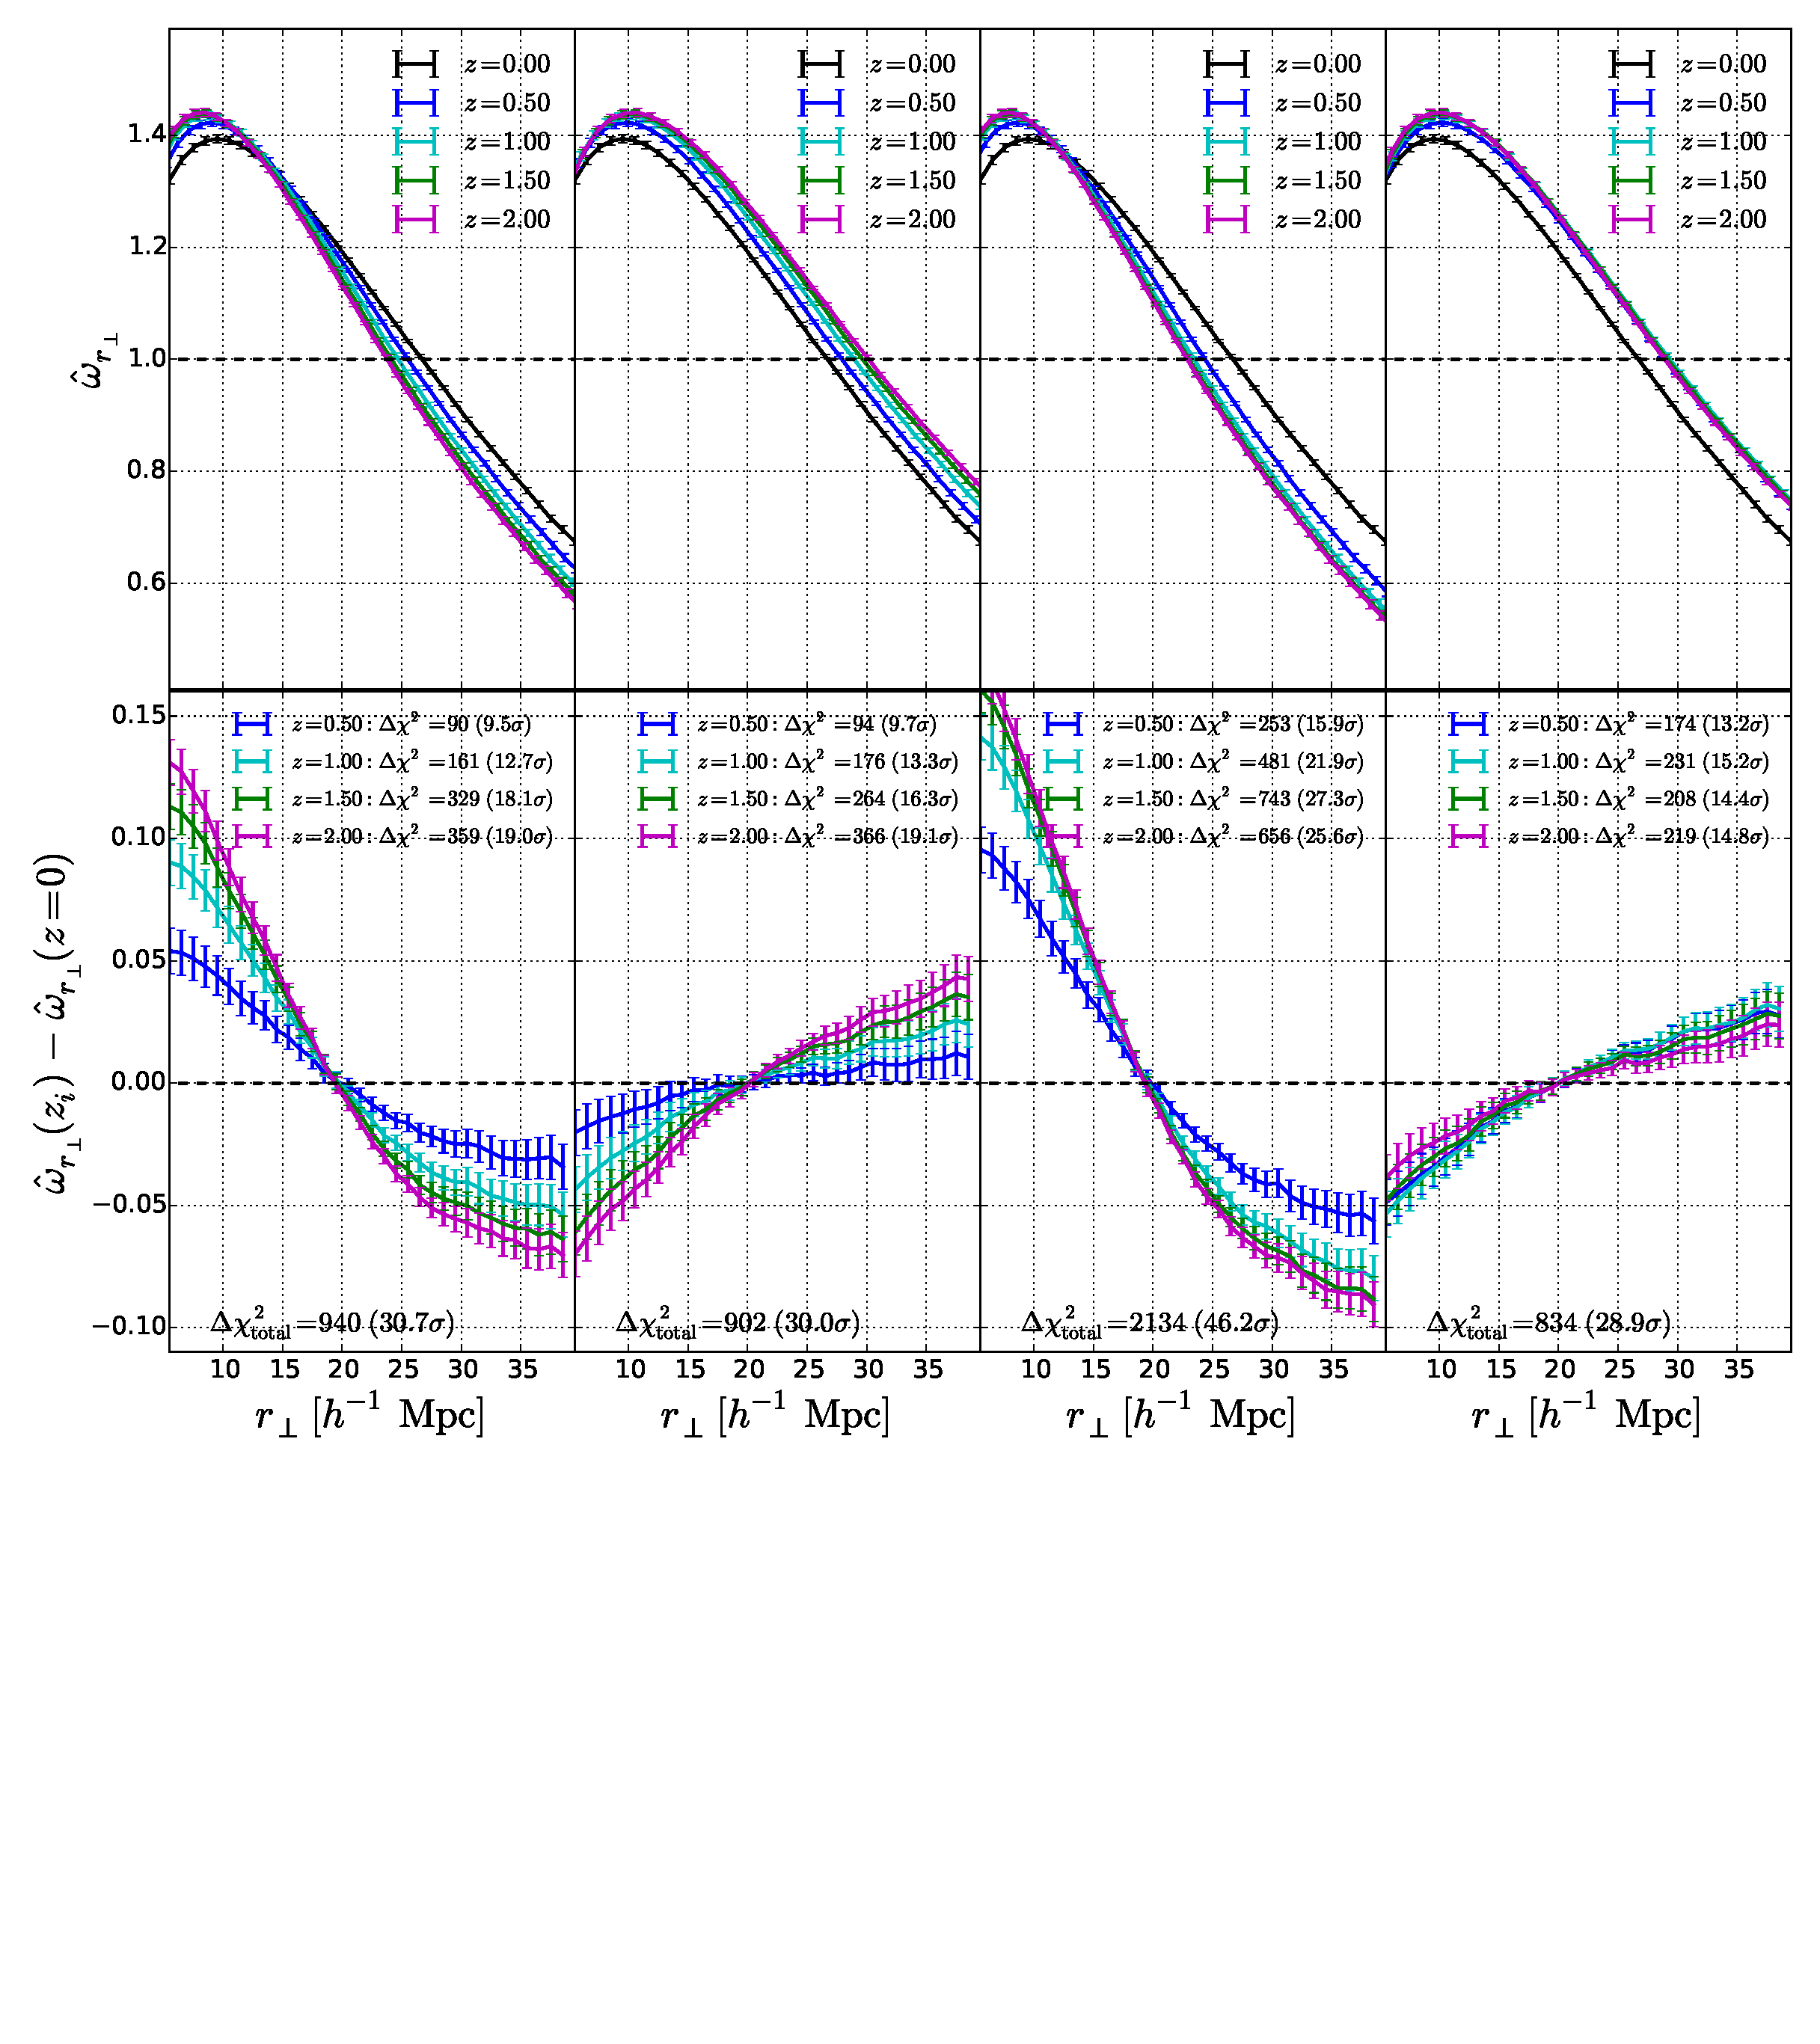
\includegraphics[width=2\columnwidth]{fig5.eps}
   }
   \caption{\label{fig_cosmo}
    $\hat{\xi}_{r_\perp}$ (upper panels) and $\hat{\xi}_{r_\perp}(z=z_i) - \hat{\xi}_{r_\perp}(z=0)$ (lower panels) at several redshifts,
    for four wrong cosmologies.
    The redshift evolution of the $\hat\xi_{r_{\perp}}$ shape in these wrong cosmologies are detected at high CL.
   }
\end{figure*}

The galaxy peculiar velocity contaminates the observed redshift and distorts 
the inferred galaxy radial position.
It is the major systematic in our previous works \citep{Li2014,Li2015,Li2016}
of statistical analysis on the 3D galaxy distribution.

The effect of RSD is much milder in this work. 
The angular positions of galaxies are not shifted by RSD at all;
the only effect of RSD enter in the procedure of 
splitting galaxies into redshift shells.
The galaxies observed in a survey are split into shells of subsamples, 
with different redshift ranges. This allows us to obtain 2pCF measurement at various redshifts.
RSD distorts the galaxy redshift and as a result some galaxies 
(especially those close to the boundaries of shells) are assigned to the wrong redshift shells.

We shift the radial coordinates of galaxies according to the relation 
\begin{equation}\label{eq:zvpeu}
\Delta z = (1+z) \frac{v_{{\rm Z}}}{c},
\end{equation}
where $v_{{\rm Z}}$ (Z is the third coordinate of the galaxy in the box, treated as the radial direction in this analysis) 
is the galaxy peculiar velocity in the LOS direction.
This lead to {\it misclassification} of some galaxies when we split the box into slices.
%Then we split the whole box into 30 slices with thickness $105h^{-1}\rm Mpc$, 
%and measure the angular 2pCF.

The upper panel of Figure \ref{fig_sys} shows how it affects on the 2pCF.
Comparing this plot with Figure \ref{fig_diffz} one can clearly see the effect of RSD.
The amplitude of the measured 2pCF is enhanced by $\sim 10\%$ when considering the RSD effect 
and the slop of $\hat\xi_{r_\perp}$ is suppressed.
However, the redshift evolution of $\hat\xi_{r_\perp}$ remains small,  $\lesssim4\%$ at $0.5\leq z \leq 2$.
Therefore RSD should not significantly affect the application of our method, as long as its redshift evolution is small;
the small effect of RSD can be precisely modelled by simulations and corrected.
%If looking at the redshift evolution,
%the curves $\hat{r_\perp\xi} - \hat{r_\perp\xi}(z=0)$ displayed in the right panel,
%they changed a lot compared with the case of no RSD effect (the right panel of Figure \ref{fig_diffz}),
%but do not become much larger. %But RSD effect does not introduce large redshfit evolution, although the shape of  is 

Similar to RSD, redshift errors of galaxies
also results in fuzzy boundaries of redshift shells.
Thankfully, there are some methods for mitigating this effect in photometric surveys using, for example, pair-center binning \citep{2010MNRAS.407..520N, 2011MNRAS.415.2193R}. 

\subsubsection{Galaxy Bias}

\begin{figure*}
   \centering{
   %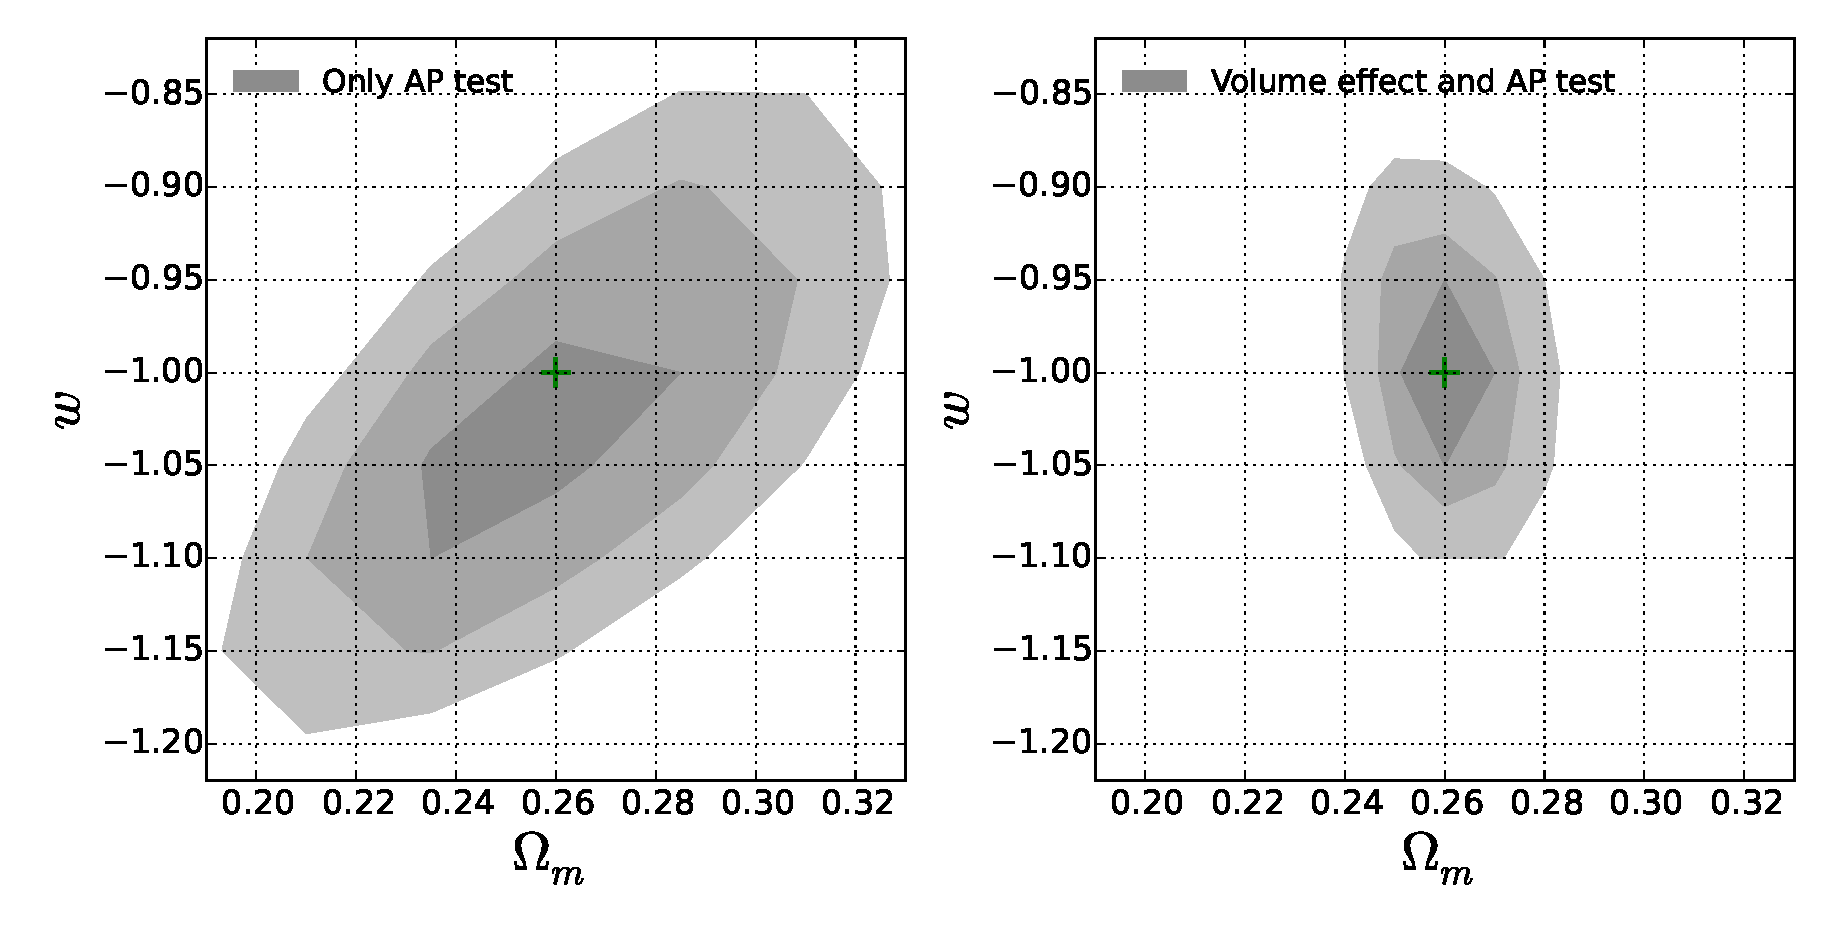
\includegraphics[width=7cm]{Tpcf--contour.eps}
   %\includegraphics[width=16cm]{Tpcf--contour-others.eps}
   %\includegraphics[width=16cm,natwidth=52,natheight=40]{fig10.eps}
   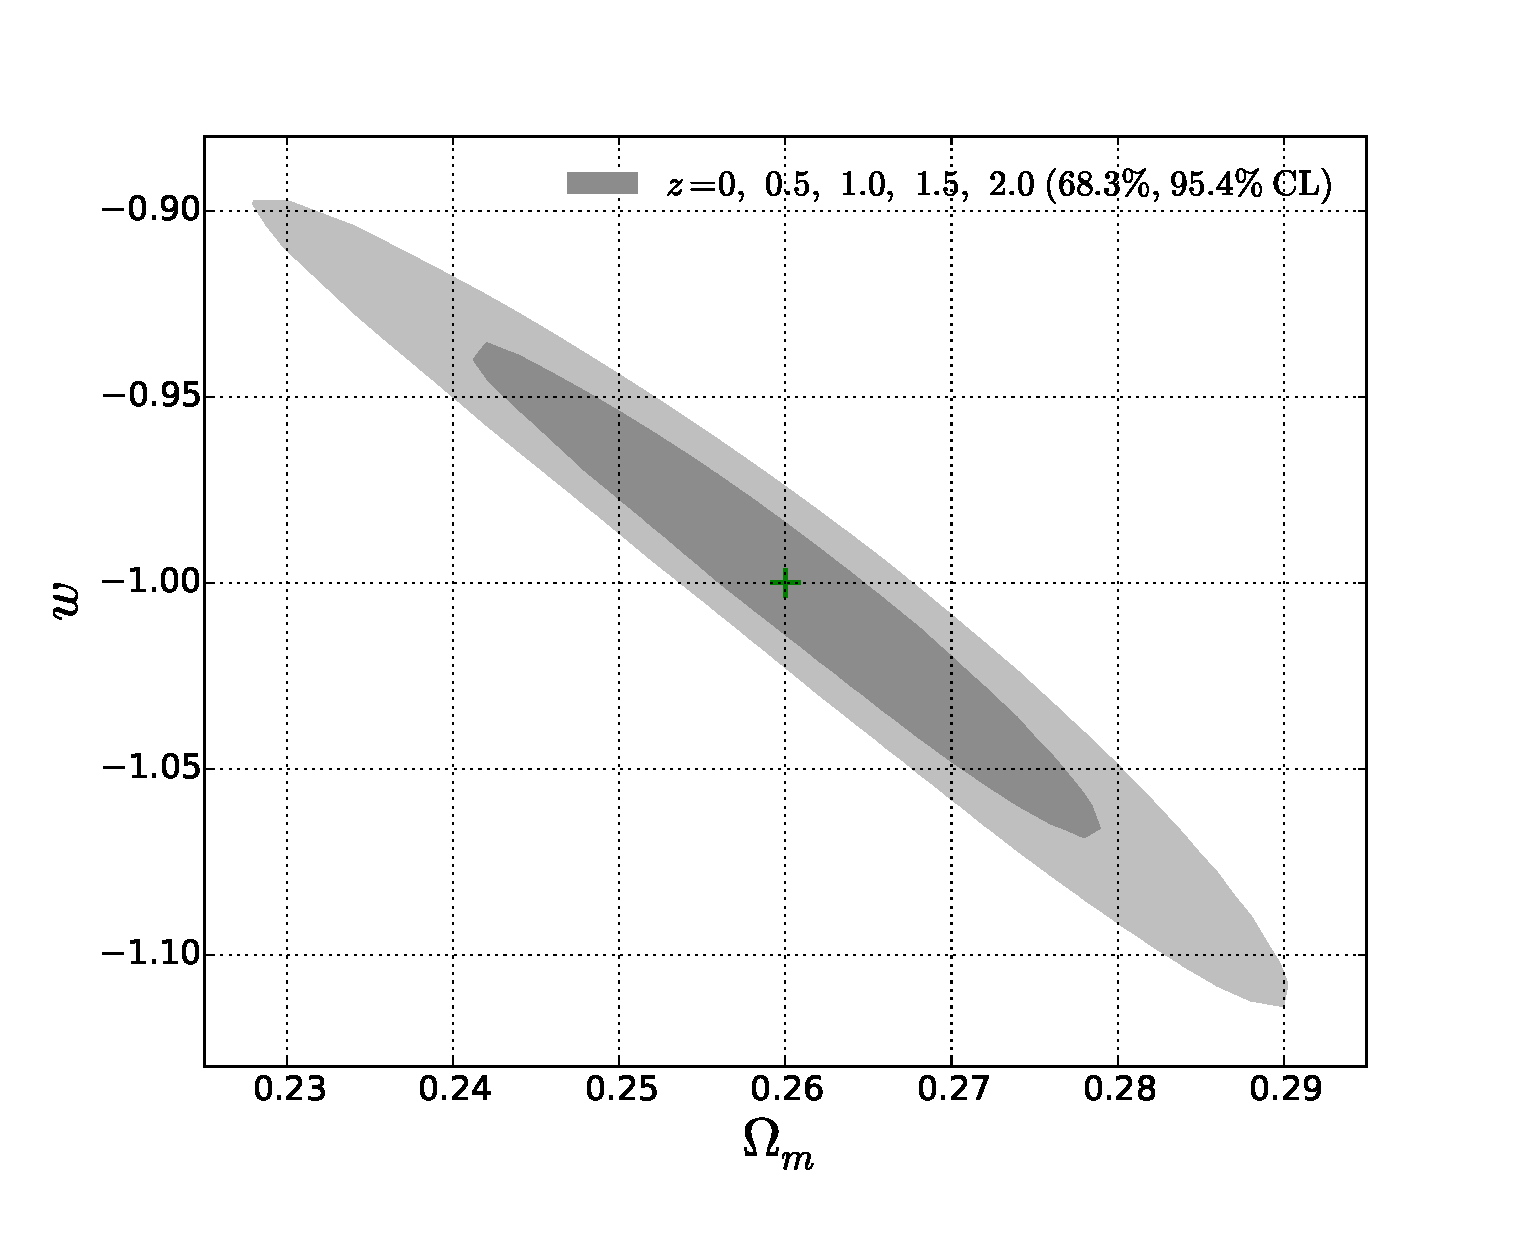
\includegraphics[width=8cm]{fig9_a.eps}
   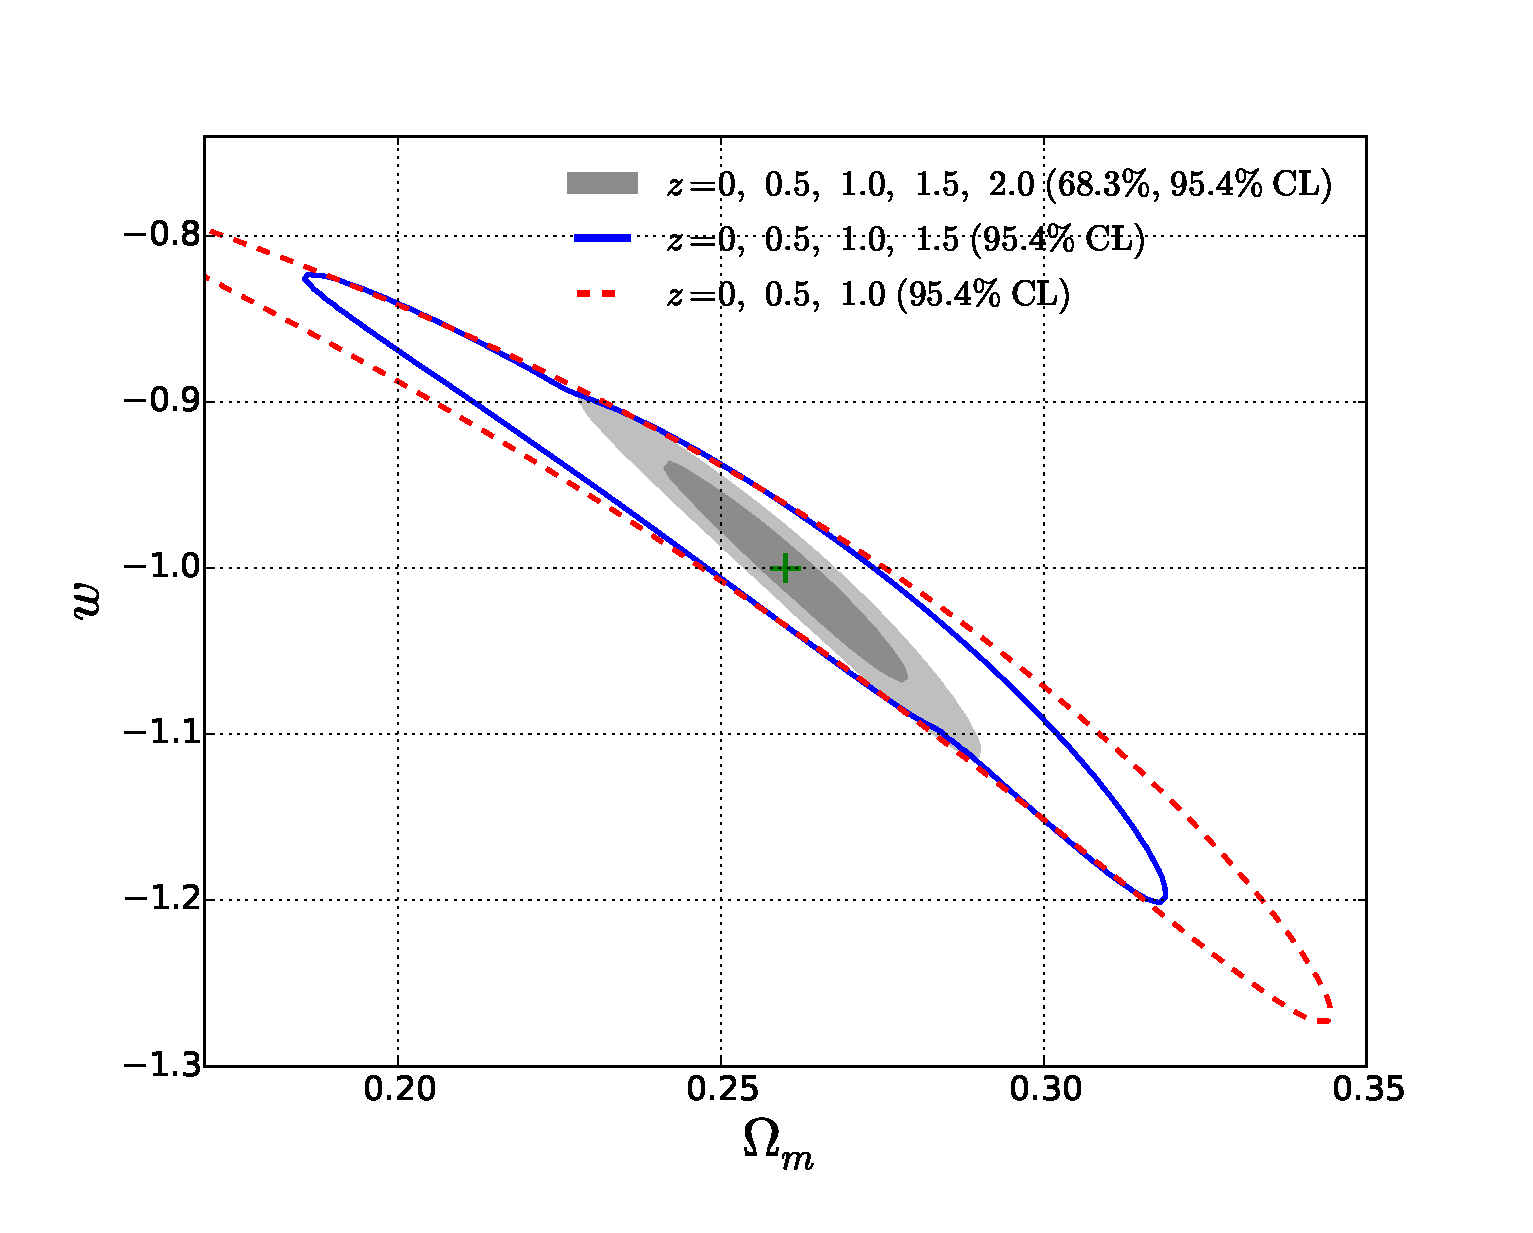
\includegraphics[width=8cm]{fig9_b.eps}
   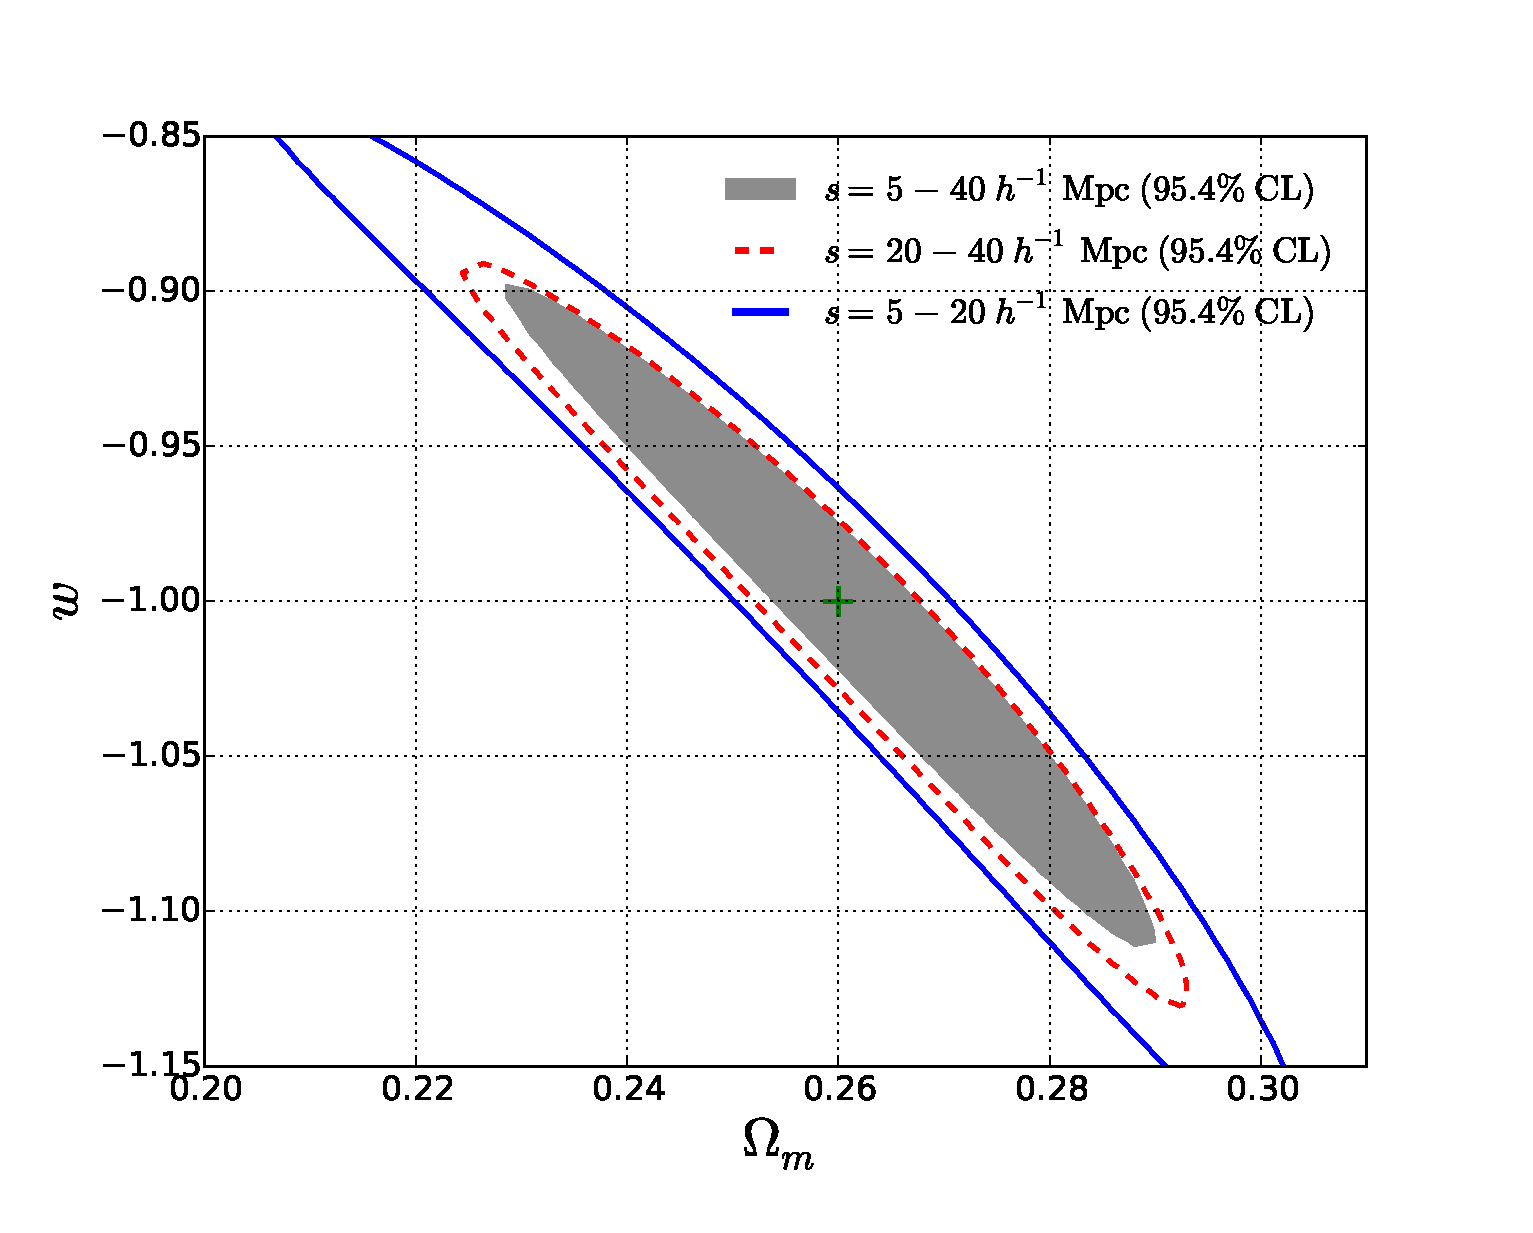
\includegraphics[width=8cm]{fig9_c.eps}
   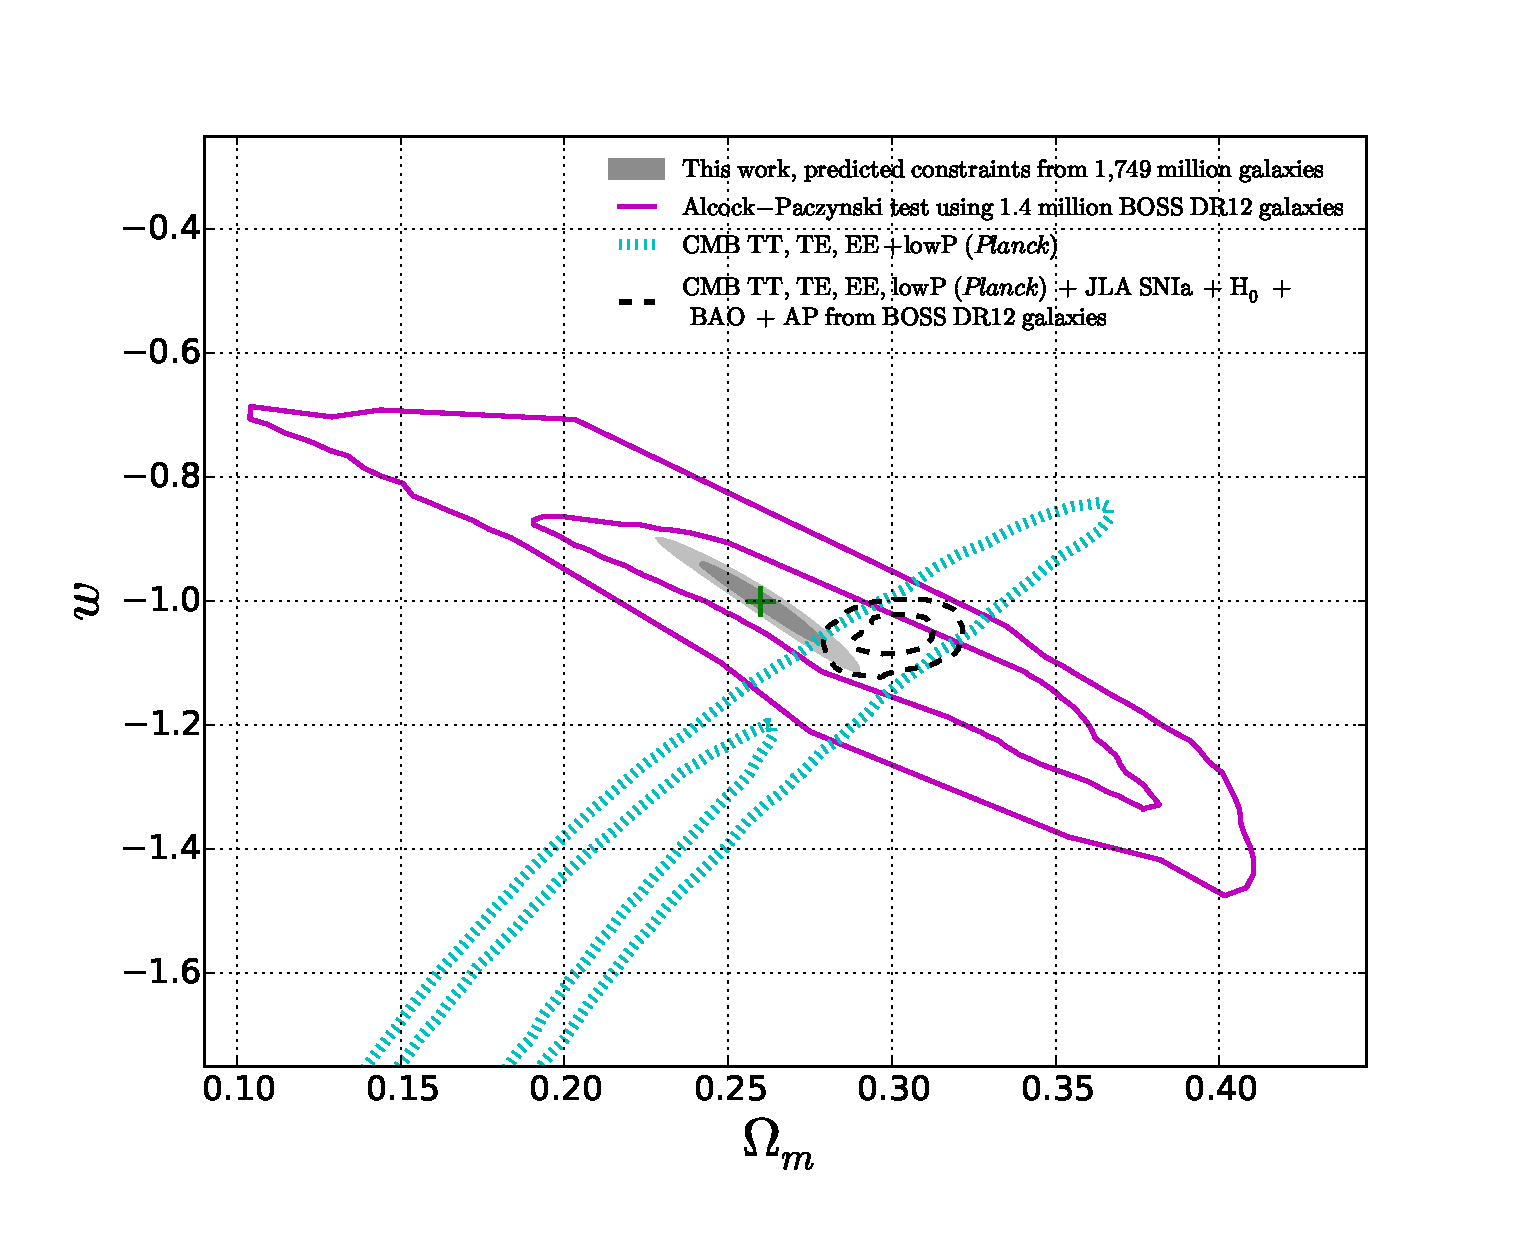
\includegraphics[width=8cm]{fig9_d.eps}
   }
   \caption{\label{fig_contours}
   Upper left: Likelihood contours (68.3\%, 95.4\%) in the $\Omega_m-w$ plane from our method, 
   based on the redshift evolution of the angular 2pCF shape $\hat\omega_{r_\perp}$.
   The green point denotes our fiducial cosmological model and the contours denote the statistical error.
   Utilizing the HR4 snapshots data (containing hundreds of millions of galaxies at redshifts 0, 0.5, 1, 1.5, 2),
   the method lead to very tight cosmological constraint.
   Upper right: The constraints in case that one or two high redshift bins are not used.
   Lower left: The 95.4\% likelihood contours using different clustering scales.
   Lower right: A comparison of the constraint with the cosmological constraints from the current observational data.
   }
\end{figure*}

Galaxies are biased tracers of the dark matter field;
more massive galaxies reside in regions with higher density contrast
and exhibit stronger clustering (i.e. larger bias).
%In large scale structure surveys, the bias of the galaxy sample is an important fator affecting on the clustering properties of the sample.

We vary the mass cut and check the effect of galaxy bias on $\hat \xi_{r_\perp}$.
The second row of Figure \ref{fig_sys} displays the 2pCF measured from galaxies within a $3150\times3150\times105$ $(h^{-1}\rm Mpc)^3$ volume, taken from the $z=0$ snapshot.
Four values of minimal mass limits, $3\times 10^{11} M_{\odot}$, $1\times 10^{12} M_{\odot}$, $4\times 10^{12} M_{\odot}$ and $1\times 10^{13} M_{\odot}$,
are imposed to create samples with different galaxy biases.
The measured 2pCF across the line-of-sight are displayed.

Different mass cuts result in large variation in the amplitude of the 2pCF (left panel);
but the shape of the normalised 2pCF remains less affected (middle panel).
Compared with the sample of $M>3\times 10^{11} M_{\odot}$,
samples with mass limits of $1\times 10^{12} M_{\odot}$, $4\times 10^{12} M_{\odot}$ and $1\times 10^{13} M_{\odot}$
have amplitude of 2pCFs enhanced by $10\%,\ 50\%$ and $100\%$, 
while the change in the shape is only $0.5\%,\ 2\%$ and $4\%$, respectively.
The effect of galaxy bias becomes much less significant by utilizing the shape of the 2pCF rather than the amplitude.

% {\bf 
The combined effect of galaxy bias and RSD results in larger systematics.
Galaxies that are more biased predominantly reside within nonlinear, over-dense regions and thus have larger larger peculiar velocities.
The third row of Figure \ref{fig_sys} shows that, 
the difference of $\hat \xi_{r_\perp}$ among different mass cut samples reaches $1.5\%,\ 4\%$ and $8\%$ in the case when including the RSD effect.

Finally, the fourth row of the Figure displays the 
redshift evolution in case of using samples with constant number density $\bar n=7.3\times 10^{-3} {\rm Mpc}^{-3}h^3$, 
with the RSD effect considered. %(the error bar is a bit larger since for an illustration purpose we only do the computation for 1/30 of the whole sample).
We see the redshift evolution of $\hat \xi_{r_\perp}$ is as small as $\lesssim3\%$.

%In summary, the effect of RSD and galaxy bias on the shape of the galaxy correlation function across the line-of-sight is not large, but is non-negligible.
%When dealing with real observational data, one should construct simulation mocks in which these effects are reliably modelled, 
%so that the systematics are corrected and will not lead to significant bias in the derived cosmological constraints.

%In \cite{Li2014,Li2015,Li2016}, the systematic effects contributing to the redshfit evolution of galaxy clusterings 
%are modeled in mock surveys and subtracted.
%Similar treatment could be conducted here.
%One shall construct mock surveys with the above effects included for the correction of systematics.


%The outer boundary of the mock survey becomes fuzzy due to the peculiar velocity effect 
%on the galaxy redshifts (Eq. (\ref{eq:zvpeu})).
%A population of galaxies, that are expected to enter the $z<0.7$ region from the outside, is missing.
%(these $z>0.7$ galaxies have a peculiar velocity toward us and 
%their observed redshfits become lower than 0.7).
%To avoid this problem we set the maximal redshift at 0.693, 
%23.3 $h^{-1}{\rm Mpc}$ away from $z=0.7$.


%3.000e11', '1.000e12', '4.000e12',  '1.000e13



\subsubsection{More discussion}

In summary, we aim to minimise the redshift evolution of the shape of the normalised  2-point correlation function across the line-of-sight; 
the shape change is dramatic when considering a cosmological model significantly different from the fiducial model.
However even in the case of the correct cosmology there remains a small signal, due to growth of structures, RSD and galaxy bias. 
These systematics are removed with the aid of simulations.
The procedure of the correction of systematics is similar to what was implemented in our previous papers \cite{Li2014,Li2015,Li2016}.

The systematics are estimated from a simulation conducted using a particular cosmology. 
Thus there could be a bias in their estimation if the simulation cosmology is different from the true cosmological model/. 
The bias would not be serious if the simulation cosmology is consistent with the best-fit cosmological parameters obtained from the analysis \cite{Li2016}. 
In the case that there is a large discrepancy between the simulation cosmology and the best-fit cosmology, one needs to adjust the simulation cosmology and re-do the analysis.

A more precise approach would involve estimating the systematic effect from a set of simulations covering the relevant volume of the parameter space. 
This would remove the remaining uncertainty associated with the cosmological dependence. 
This approach would also enable the estimation of the $systematic\ error$, 
which could be important when the sample size is large enough and the systematic error becomes as small as the $statistical\ error$.

The third row of Figure \ref{fig_sys} shows that, 
if having a large difference in galaxy bias between the samples,
there is a large systematic variation on small scales. 
This means that accurate modelling of systematics from simulations is required. 
In an effort to mitigate this problem, one can conduct the analysis using a volume-limited galaxy sample, 
where the redshift evolution of galaxy properties is small and the systematic effect from RSD and galaxy bias is also small,
as shown by the fourth row of Figure \ref{fig_sys}.

To avoid the large systematics in the nonlinear regime, 
another solution would be to increase the scale of analysis to larger separations where the non-linear effect is becoming subdominant. 
Figure \ref{fig_sys} shows that, 
on scales of $s=20-50 h^{-1} {\rm Mpc}$ the systematic effect is 2-3 times smaller than that of $s=5-20 h^{-1} {\rm Mpc}$. 
Actually, we tested and found that, using $s = 5-40 h^{-1} {\rm Mpc}$ and $20-40 h^{-1} {\rm Mpc}$, 
yields cosmological constraints that are pretty close to each other (see \S 4). 

We do not consider the systematic effects in case of non-standard cosmological scenarios such as modified gravity and warm dark energy. 
These topics go beyond the scope of this work, however they are worthy future investigations.


\subsection{Likelihood Analysis}


Adopting the correct cosmological model will result in minimal evolution of the normalised 2pCF.
Thus we proceed to construct a quantitative likelihood estimator that reflects this property.
The procedure here is very similar to \cite{Li2014,Li2015,Li2016}.
We compare the high redshift $\hat\xi_{r_\perp}$ and the lowest redshift measurement,
\begin{equation}
 \delta \hat{\xi_{r_\perp}}(z_i,z_1) \equiv \hat{\xi_{r_\perp}}(z_i) - \hat{\xi_{r_\perp}}(z_1),
\end{equation}
and design the likelihood function to quantify
the redshift evolution of $\hat\xi_{r_\perp}$:
\begin{equation}\label{eq:chisq1}
\chi^2\equiv \sum_{i=2}^{n_{z}} \sum_{j_1=1}^{n_{r}} \sum_{j_2=1}^{n_{r}} {\bf p}(z_i,r_{j_1}) ({\bf Cov}_{i}^{-1})_{j_1,j_2}  {\bf p}(z_i,r_{j_2}),
\end{equation}
where $n_z$ is the number of redshifts bins, which is 5 in this analysis, 
$n_r$ is number of binning in $\hat{\xi}_{r_\perp}(r_\perp)$,
which is 35 since we have $r_\perp$ bins 
with width $1h^{-1}\rm Mpc$ in a range of $5h^{-1}{\rm Mpc}\leq r_\perp\leq 40h^{-1}{\rm Mpc}$.
${\bf p}(z_i,r_{j})$ is the redshift evolution of the correlation function shape with systematic effects subtracted
\begin{eqnarray}\label{eq:bfp}
 {\bf p}(z_i,r_{j}) \equiv&\ \delta \hat{\xi_\perp}(z_i,z_1,r_j) - \delta \hat{\xi}_{r_\perp,\rm sys}(z_i,z_1,r_j)
\end{eqnarray}
${\bf Cov}_i$ is the covariance matrix estimated from the ${\bf p}(z_i,r_{j})$ measured from 120 subsamples.
%It is difficult to conduct the 2pCF of the whole snapshot box with hundreds of millions of galaxies.
%We split the box into 120 subsamples with $X,Y,Z$ sizes of $1575h^{-1}{\rm Mpc},1575h^{-1}{\rm Mpc}, 105h^{-1}{\rm Mpc}$
%and measure the angular 2pCF in the $X-Y$ plan in these subsamples. 
%The average of the 2pCFs are taken as the 2pCF of the whole box.
%The covariance matrix is also estimated from the redshift evolution of these subsamples.
As mentioned previously, for a robust estimation of the covariance matrix, 
we always compare slices at different locations to 
include the cosmic variance.

The covariance matrix inferred from a finite number of samples
is always a biased estimate of the true matrix \citep{Hartlap}.
This can be corrected by rescaling the inverse covariance matrix as 
\begin{equation}
 {\bf Cov}^{-1}_{ij,\rm Hartlap} = \frac{N_s - n_{r}-2}{N_s-1} {\bf Cov}^{-1}_{ij},
\end{equation}
where $N_s=120$ is the number of mocks used in covariance estimation.
For this analysis the rescaling is as large as 1.43.
In the case that one has 2\,000 mocks the rescaling is less than 1.02.


%estimated from the 72 sets of PSB mock galaxies identified from HR3 N-body simulation.


Figure \ref{fig_cosmo} displays the 2pCF and the likelihood values when adopting 
the four incorrect cosmologies used in Figure \ref{fig_xyquan}.
For the cosmologies $\Omega_m=0.4,w=-1$ and $\Omega_m=0.26,w=-0.5$,
the compression shifts the clustering patterns to smaller scales
at higher redshift and make the 2pCFs steeper.
%and also becomes more significant at higher redshift.
%We get 2pCFs with steeper slope and the higher redshift the steeper.
For the cosmologies $\Omega_m=0.15,w=-1$ and $\Omega_m=0.26,w=-1.5$,
the stretch of structure leads to a shallower slope of $\hat{\xi}_{r_\perp}$ at higher redshift.
%the shallower.
In all cosmologies there is significant detection of redshift evolution.
We compute the $\chi^2$ values according to Equation \ref{eq:chisq1}, 
and find that these cosmologies are disfavored 
at $\gtrsim30\sigma$ CL.






\section{Cosmological constraint}


We constrain $\Omega_m$ and $w$ through a Bayesian analysis (\cite{Bayesian}; also see \cite{LB2002,Li2016}).
We assume that the likelihood takes the form
\begin{equation}\label{eq:like}
 \mathcal{L} \propto \exp\left[-\frac{\chi^2}{2}\right],
\end{equation}
and scan the parameter space in the $\Omega_m-w$ plane to obtain the 68.3\% and 95.4\% CL regions.
The result is displayed in the left panel Figure \ref{fig_contours}.


We obtain tight constraints on the two parameters.
The 2$\sigma$ contour lies within the region $0.23<\Omega_m<0.29$, $-1.1<w<-0.9$.
The two parameters are very strongly degenerated with each other,
and the area of constrained region is quite small.
The thin shape of the contour implies that, 
when combining with other observational data with a different direction of degeneracy (e.g. CMB, BAO),
a very tight combined constraint can be obtained.

In the case of fixing one parameter at its best-fit value and constraining the other,
one obtains very small 1$\sigma$ uncertainties of $\delta\Omega_m\approx0.003,\delta w\approx0.01$.

The simulation sample used in this analysis reaches $z=2$.
The constraint becomes weaker if we limit the highest redshift of the samples.
The upper right panel displays that, 
in case that we exclude the $z=2$ galaxies, 
the 2$\sigma$ uncertainties of $\delta\Omega_m\approx0.01,\\ \delta w\approx0.1$ (the other parameter fixed at its best-fit value).
The area of contour is further enlarged by $\approx 50\%$ if we only use galaxies at $z=$0, 0.5 and 1.

So far we simply follow the convention of \cite{Li2016} and adopt $5\hMpc <s< 40\hMpc$ as our analysis scale. 
As discussed in the \S 4.3.3, one may want to avoid large systematics in the non-linear regime. 
In this case one may adopt $20\hMpc<s<40\hMpc$,
which significantly reduces the systematic effects but does not degrade the power of the parameter constraints,
as shown by the lower left panel of Figure \ref{fig_contours}.

The choice of the redshift width $105 \hMpc$ is also slightly little arbitrary. 
It should be larger than the distance distortion from the RSD and redshift errors.
The optimistic scheme of clustering scales and redshift width should depend on the specific galaxy sample used in the analysis. 
One could adjust them to have a good balance between the power of cosmological constraint and the size of systematic effect.

Finally, to be connected with the real observations, 
the lower right panel displays the constraints from Planck CMB (dotted blue, \cite{Planck2015}),
the AP analysis using BOSS DR12 galaxies (solid magenta, \cite{Li2016}),
and the joint constraint $\Omega_m = 0.301 \pm 0.006,\ w=-1.054 \pm 0.025$ 
obtained using the CMB+SNIa+BAO+AP (dashed black, \cite{6dFGS,MGS,Riess2011,JLA,Anderson2013,Li2016}).

The predicted constraints from this method clearly wins due to the large sample size.
The total number of galaxies used in this work is 1,749 million,
which is 1,000 times of the BOSS DR12 sample size.
So the constrained area is also $\sim 30$ times smaller.
Such a large sample size will be enabled by LSST (the Large Synoptic Survey Telescope) \footnote{https://www.lsst.org/}, 
which probe tens of billions of galaxies at $z\lesssim2$.


%combined with an AP analysis using BOSS DR12 galaxies. This represents the current scenario of cosmological constraints from observations. A new plot is added to compare it with the constraint from our method.
%the JLA SNIa sample (green area, ),
%the BAO measurement from BOSS DR11 galaxies (bright yellow, ),
%\footnote{The CMASS and LOWZ samples from BOSS DR11 have a sky coverage of 8\,377 $\rm deg^2$ and a completeness of 97\%.
%They are very close to the DR12 samples.},
%a combination of the BOSS DR11 BAO and the Hubble Space Telescope measurement of $H_0=70.6\pm3.3$ (dark yellow, ),
%and the full-mission Planck observations of temperature and polarization anisotropies, released in 2015 (blue, \cite{Planck2015})

\section{Concluding Remarks}
 
We have developed a method for constraining certain cosmological parameters by measuring the redshift evolution of the shape of the galaxy 2pCF across the line-of-sight, $\hat \xi_{r_\perp}$.
We found that a wrongly adopted cosmology results in a redshift-dependent mis-scaling in the constructed galaxy distribution,
which in turn leads to a redshift-dependent rescaling of $\hat \xi_{r_\perp}(r_\perp)$.
The redshift dependent effect is sensitive to cosmology while being relatively insensitive to the gravitational growth of structure,
the galaxy bias, and the RSD effect.
We tested our method on the HR4 mock galaxies having 457, 406, 352, 306 and 228 million galaxies at redshifts 0, 0.5, 1, 1.5, 2.
Analyzing the redshift evolution of $\hat \xi_{r_\perp}(r_\perp)$ 
on scales $5  h^{-1} {\rm Mpc} \leq r_\perp \leq 40 h^{-1} {\rm Mpc}$, 
we derive tight constraints on $\Omega_m$ and $w$.

 
In this analysis we restrict our focus to the rescaling in the direction perpendicular to line-of-sight .
%The angular correlation function is adopted as a statistical tool to probing the scaling effect in the angular direction.
One can also use the 2D 2pCF $\xi(s,\mu)$ 
as a function of both angular and radial scale to fully probe the scaling effect in the 3D galaxy distribution.

In our early work of \cite{Li2015,Li2016}, 
we proposed to use the angular-dependence of the galaxy clustering to apply an AP test and derive cosmological constraints. 
In contrast, in this work we focus on the scale-dependence of the clustering. 
The two methods focus on different parts of the clustering information, and the constraints derived from the them should be fairly independent.
However, it is advisable to have an estimation of the covariance between them in the case there one is using both methods in combination.
An alternative way is to investigate the redshift evolution of the correlation map $\xi(s,\mu)$ as a function of both scale and direction, which captures all the information.

There are already works using the angular 2pCF to constrain cosmology
by directly comparing the theoretical 2pCF and the observed one \citep{Salvador2014,Salvador2016}.
Our method is simpler and just uses the fact that in the correct cosmology the shape of the 2pCF across the line-of-sight
does not exhibit significant redshift evolution.
%is insensitive to redshift in correct cosmology.
Our method is complementary to these works in that
it does not require accurate analytic modeling, 
and could be applicable on smaller scales. 
%The two different approaches can be combined together to fully extract the cosmological information.
 

\cite{Li2015,Li2016} shows that using the redshift dependence of the AP effect, 
one can derive very tight cosmological constraints.
The method presented in this paper studies the redshift evolution of the volume effect.
%We hope this method also.
These two methods probe different information encoded in the 2pCF 
and can be combined to give a complete geometric probe of the LSS galaxy distribution.
%Or one can also use the redshift evolution of 2D 2pCF xi(s,mu) to have all information included.

This method is designed to be applied to current and future LSS surveys,
with a particular emphasis on {\it photometric surveys}.
The galaxy 2pCF across the line-of-sight in redshift shells is much less affected by the large redshift errors compared wit the 3D 2pCF.
The Dark Energy Survey will probe hundreds of millions of galaxies at $z\lesssim1.5$
\footnote{https://www.darkenergysurvey.org/}, 
and LSST will probe tens of billions of galaxies at $z\lesssim2$.
We expect very tight cosmological constraints from these surveys.
%and the redshift error will not quite affect the angular 2pCF measurement 
%as long as the redshift dependence of the photometric redshift can be reliably understood.


Our series of works \cite{Li2014,Li2015,Li2016}, together with this analysis, 
and also \cite{topology,MS2016},
are introducing a new strategy to constrain cosmology from galaxy clustering.
We utilize a statistical pattern which remains constant at all redshifts;
this invariance is broken when incorrect cosmologies are adopted to construct the galaxy distribution
and introduces redshift evolution of geometric distortion.
The systematic effects can be corrected by performing an N-body simulation 
in a cosmology with values of parameters close enough to the underlying correct one.
This avoids the difficulty in the analytical modeling the galaxy clustering, galaxy bias and RSD,
and enables reliable cosmological constraint on relatively small clustering scales.
We hope these methods play an important role in deriving cosmological constraints from future LSS surveys.

 
 
\section*{Acknowledgments}

We thank the Korea Institute for Advanced Study for providing computing resources (KIAS Center for Advanced Computation Linux Cluster System).
%We thank Seokcheon Lee and Graziano Rossi for many helpful discussions.
We would like to thank Stephen Appleby and Yi Zheng for kind helps and valuable comments.
This work was partially supported by the
Supercomputing Center/Korea Institute of Science and
Technology Information with supercomputing resources
including technical support (KSC-2013-G2-003).

%\appendix
%\

\begin{thebibliography}{}

\bibitem[Ade et al. (2015)]{Planck2015}
Ade, P.A.R., Aghanim, N., \& Arnaud, M., et al. arXiv:1502.01589

\bibitem[Alam et al.(2016)]{Alam2016}
Alam, S., Ata, M., \& Bailey, S., et al. 2016,
submitted to MNRAS (arXiv:1607.03155)

%\bibitem[{{Alam} {et~al}\mbox{.}(2015{\natexlab{a}}){Alam}, {Albareti},
%  {Allende Prieto}, {Anders}, {Anderson}, {Anderton}, {Andrews}, {Armengaud},
%  {Aubourg}, {Bailey}, \& et~al.}]{dr12}
%{Alam} S., Albareti, F.D.,\& Allende Prieto, C., {et~al.}, 2015,  ApJS, 219, 12

\bibitem[Alcock \& Paczynski(1979)]{AP1979}
Alcock, C., \& Paczynski, B. 1979, Nature, 281, 358  

%\bibitem[Anderson et al.(2012)]{2012MNRAS.427.3435A} 
%Anderson, L., Aubourg, E., Bailey, S., et al.\ 2012, MNRAS, 427, 3435

\bibitem[Anderson et al.(2013)]{Anderson2013}
Anderson, L., Aubourg, \'E., \& Bailey, S. et al. 2014, MNRAS, 441, 24  
  
%\bibitem[Bassett et al.(2002)]{Bassett2002}
%Bassett, B.A., Kunz, M., Silk, J., \& Ungarelli, C. 2002, MNRAS, 336, 1217

\bibitem[Ballinger, Peacock \& Heavens 1996]{Ballinger1996}
Ballinger, W.E., Peacock, J.A., \& Heavens, A.F. 1996, MNRAS, 282, 877  

\bibitem[Betoule et al.(2014)]{JLA}
Betoule, M., Kessler, R., \& Guy, J., et al. 2014, A\&A, 568, 32


\bibitem[Beutler et al.(2011)]{6dFGS}
Beutler, F., Blake, C., \& Colless, M., et al. 2011, MNRAS, 416, 3017

\bibitem[Beutler et al.(2013)]{Beutler2013}
Beutler, F., Saito, S., \& Seo, H.-J., et al. 2013, MNRAS, 443, 1065

\bibitem[Beutler et al.(2016)]{Beutler2016}
Beutler, F., Seo, H.-J., \& Saito, S., et al. 2016,
arXiv:1607.03150

\bibitem[Bernardeaua et al.(2002)]{BCGS2001}
Bernardeaua, F., Colombib, S., Gaztañagac, E., \& Scoccimarro, R. 
2002, Phys.Rept., 367, 1

\bibitem[Blake \& Glazebrook (2003)]{BG03}
Blake, C., \& Glazebrook, K. 2003, ApJ, 594, 665


\bibitem[Blake et al.(2011)]{Blake2011}
Blake, C., Glazebrook, K., \& Davis, T. M., 2011, MNRAS, 418, 1725  

%\bibitem[Blake et al.(2013)]{WiggleZtopoloy}
%Blake, C., James, J.B., \& Poole, G.B. 2013, MNRAS, 437, 2488

%\bibitem[Bolton et al.(2012)]{Bolton2012}
%Bolton, A.S., Schlegel, \& D.J., Aubourg E., et al. 2012, AJ, 144, 144

%\bibitem[Boylan-Kolchin et al.(2008)]{B08}
%Boylan-Kolchin, M., Ma, C.-P., \& Quataert, E. 2008, MNRAS, 383, 93


\bibitem[Bueno Belloso et al. (2012)]{BB2012}
Bueno Belloso, A., Pettinari, G.W., Meures, N., \& Percival, W.J. 2012, Phys. Rev. D, 86, 023530

%\bibitem[Chevallier \& Polarski(2001)]{CP2001}
%Chevallier, M., Polarski, D. 2001, Int. J. Mod. Phys. D, 10, 213


%\bibitem[Choi et al.(2010)]{choi 2010}
%Choi, Y.-Y., Park, C., Kim, J., Gott, J.R., 
%Weinberg, D.H., Vogeley, M.S., \& Kim, S.S. 2010, ApJS, 190, 181

\bibitem[Christensen et al.(2001)]{Bayesian}
Christensen, N., Meyer, R., Knox, L., \& Luey, B. 2001, Class. Quant. Grav., 18, 2677

%\bibitem[Chuang et al.(2013)]{Chuang2013}
%Chuang, C.-H., Prada, F., Beutler, F., et al. 2013, arXiv:1312.4889  

\bibitem[Chuang \& Wang(2012)]{ChuangWang2012}
Chuang, C.-H., \& Wang, Y. 2012, MNRAS, 426, 226  


%\bibitem[Corasaniti \& Copeland(2003)]{Corasaniti2003}
%Corasaniti, P.S., Copeland, E.J. 2003, Phys. Rev. D, 67, 063521

%eBOSS: 
%http://arxiv.org/abs/1508.04473
%\bibitem[Dawson et al.(2015)]{eBOSS}
%Dawson, K.S., Kneib, J.P., \& Percival, W.J., et al. 2015, accepted AJ

%\bibitem[Dawson et al.(2012)]{Dawson et al. 2012}
%Dawson, K.S., Schlegel, D.J., \& Ahn, C.P., et al. 2012, AJ, 145, 10

%\bibitem[Efstathiou (2014)]{E14H}
%Efstathiou, G. 2014, MNRAS, 440, 1138

\bibitem[Eisenstein et al. (1998)]{EHT1998}
Eisenstein, D.J., Hu, W., \& Tegmark, M. 1998, ApJ, 504, L57


%\bibitem[Eisenstein et al.(2011)]{Eisenstein et al. 2011}
%Eisenstein, D.J.,  Weinberg, D.H., \& Agolet, E., et al. 2011, AJ, 142, 72



%\bibitem[Feldman, Kaiser \& Peacock (1994)]{1994ApJ...426...23F} 
%Feldman, H.A., Kaiser, N., \& Peacock, J.A.\ 1994, ApJ, 426, 23 

%\bibitem[Fukugita et al. (1996)]{Fukugita1996}
%Fukugita, M., Ichikawa, T., \& Gunn, J.E., et al. 1996, AJ, 111, 1748
%Publication:	
%Astronomical Journal v.111, p.1748 

%\bibitem[Gingold \& Monaghan(1977)]{GM1977}
%Gingold, R.A., \& Monaghan, J.J. 1977, MNRAS, 181, 375  

%\bibitem[Gott et al.(2009)]{gott 2009}
%Gott, J.R., Choi, Y.-Y., Park, C., \& Kim, J. 2009, ApJ, 695, L45  

%\bibitem[Gott et al.(2008)]{gott 2008}
%Gott, J.R., Hambrick, D.C., Vogeley, M.S., Kim, J., Park, C., Choi, Y.-Y.,
%Cen, R., Ostriker, J.P., \& Nagamine, K. 2008, ApJ, 675, 16  


%\bibitem[Gunn et al. (1998)]{Gunn1998}	
%Gunn, J.E., Carr, M., \& Rockosi, C. et al. 1998, AJ, 116, 3040

%\bibitem[Gunn et al.(2006)]{Gunn et al. 2006}
%Gunn, J.E., Siegmund, W.A., \& Mannery, E.J., et al. 2006, AJ, 131, 2332

%\bibitem[Guzzo et al.(2008)]{Guzzo2008}
%Guzzo, L., Pierleoni, M., \& Meneux, B., et al. 2008, Nature, 451, 541

\bibitem[Hartlap et al.(2006)]{Hartlap}
Hartlap J., Simon P. \& Schneider P. [astro-ph/0608064].


\bibitem[Hong et al.(2016)]{hong2016}
Hong, S.E., Park, C.,\&  Kim, J. 2016, ApJ, 823, 103

\bibitem[Jackson (1972)]{FOG}
Jackson, J., 1972, MNRAS, 156, 1

\bibitem[Jennings et al.(2011)]{Jennings2011}
Jennings, E., Baugh, C.M., \& Pascoli, S. 2011, MNRAS, 420, 1079  

\bibitem[Jeong et al.(2014)]{Jeong2014}
Jeong, D., Dai, L., Kamionkowski, M., \& Szalay, A.S. 2014, arXiv:1408.4648

\bibitem[Jiang et al.(2008)]{jiang2008}
Jiang, C.Y., Jing, Y. P., \& Faltenbacher, A., et al. 2008, ApJ, 675, 1095

\bibitem[Kaiser (1987)]{Kaiser1987}
Kaiser, N. 1987, MNRAS, 227, 1


%\bibitem[Kim \& Park(2006)]{kim and park 2006}
%Kim, J., \& Park, C. 2006, ApJ, 639, 600  

%\bibitem[Kim et al.(2009)]{2009ApJ...701.1547K} 
%Kim, J., Park, C., Gott, J.R., III, \& Dubinski, J.\ 2009, ApJ, 701, 1547 

\bibitem[Kim et al.(2015)]{hr4}
Kim, J., Park, C., L'Huillier, B., \& Hong, S. E. 2015, JKAS, 48, 213

\bibitem[Kim et al.(2011)]{horizonrun}
Kim, J., Park, C., Rossi, G., Lee, S.M., \& Gott, J.R. 2011, JKAS, 44, 217  


\bibitem[Nock et al.(2010)]{2010MNRAS.407..520N} Nock, K., Percival, W.~J., \& Ross, A.~J.\ 2010, \mnras, 407, 520 

%\bibitem[Kitaura et al.(2015)]{MDPATCHY}
%Kitaura, F.S., Rodrı\'{i}guez-Torres, S., Chuang, C.-H., et al. arXiv:1509.06400

\bibitem[Komatsu et al.(2011)]{komatsu 2011}
Komatsu, E., Smith, K. M., \& Dunkley, J., et al. 2011, ApJS, 192, 18  

%\bibitem[Lacey \& Cole(1993)]{LC93}
%Lacey, C., \& Cole, S. 1993, MNRAS, 262, 627


\bibitem[Landy \& Szalay(1993)]{1993ApJ...412...64L} 
Landy, S.D., \& Szalay, A.S.\ 1993, ApJ, 412, 64 

%EUCLID:
%http://arxiv.org/abs/1110.3193
%\bibitem[Laureijs et al.(2011)]{EUCLID}
%Laureijs, R., Amiaux, J., \& Arduini, S., et al. 2011, arXiv:1110.3193

\bibitem[Lavaux \& Wandelt(2012)]{LavausWandelt1995}
Lavaux, G., \& Wandelt, B.D. 2012, ApJ, 754, 109  

%\bibitem[Levi et al.(2013)]{2013arXiv1308.0847L} 
%Levi, M., Bebek, C., Beers, T., et al.\ 2013, arXiv:1308.0847 

\bibitem[Lewis \& Bridle (2002)]{LB2002}
Lewis, A., \& Bridle, S. 2002, Phys. Rev. D, 66, 103511

%\bibitem[L'Huillier et al.(2014)]{2014NewA...30...79L} 
%L'Huillier, B., Park, C., \& Kim, J.\ 2014, New Astronomy, 30, 79 

\bibitem[Li et al.(2011)]{Li2011}
Li, M., Li, X.-D., Wang, S., \& Wang, Y. 2011, Commun. Theor. Phys., 56, 525

\bibitem[Li et al.(2014)]{Li2014}
Li, X.-D., Park, C., Forero-Romero, J., \& Kim, J. 2014, ApJ, 796, 137

\bibitem[Li et al.(2015)]{Li2015}
Li, X.-D., Park, C., Sabiu, C.G., \& Kim, J. 2015, MNRAS, 450, 807 

\bibitem[Li et al.(2016)]{Li2016}
Li, X.-D., Park, C., Sabiu, C.G., \& Kim, J. 2016, submitted to ApJ


%\bibitem[Linder(2003)]{Linder2003}
%Linder, E.V. 2003, Phys. Rev. Lett., 90, 091301

\bibitem[Linder et al.(2014)]{Linder2013}
Linder, E.V., Minji, O., Okumura, T., Sabiu, C.G., \& Song, Y.-S. 2014, Phys. Rev. D, 89, 063525  

\bibitem[L{\'o}pez-Corredoira(2014)]{2014ApJ...781...96L} 
L{\'o}pez-Corredoira, M.\ 2014, ApJ, 781, 96 

\bibitem[Mao et al. (2016)]{Qingqing2016}
Mao, Q., Berlind, A.A., Scherrer, R.J., et al. 2016, submitted to ApJ

\bibitem[Marinoni \& Buzzi(2010)]{Marinoni2010}
Marinoni, C., \& Buzzi, A. 2010, Nature, 468, 539  

\bibitem[Matsubara \& Suto(1996)]{Matsubara1996}
Matsubara T., \& Suto, Y. 1996, ApJ, 470, L1  

%\bibitem[McCavana et al.(2012)]{M12}
%McCavana, T., Micic, M., Lewis, G. F., et al. 2012, MNRAS, 424, 361


\bibitem[Morandi \& Sun (2016)]{MS2016}
Morandi, A., \& Sun, M. arXiv:1601.03741


\bibitem[Outram et al.(2004)]{Outram2004}
Outram, P.J., Shanks, T., Boyle, B.J., Croom, S.M., Hoyle, F., Loaring, N.S., 
Miller, L., \& Smith, R.J. 2004, MNRAS, 348, 745  

\bibitem[Parejko et al.(2013)]{Parejko2013}
Parejko J.K., et al., 2013, MNRAS, 429, 98

%\bibitem[Parihar et al. (2014)]{CMASSLSS2014}
%Parihar, P., Vogeley, M.S., \& Gott, J.R., et al. 2014, ApJ, 796, 86

%\bibitem[Park et al.(2005)]{park 2005}
%Park, C., Kim, J., \& Gott, J.R. 2005, ApJ, 633, 1  

\bibitem[Park \& Kim(2010)]{topology}
Park, C., \& Kim, Y.-R. 2010, ApJL, 715, L185  

%\bibitem[Park et al. (2012)]{Park2012}
%Park, C., Choi, Y.-Y., Kim, J., Gott, J.R., Kim, S.S., \&
%Kim, K.-S. 2012, ApJ, 759, 7

%\bibitem[Park et al. (2015)]{Park2015}
%Park, C., Song, H., Einasto, M., Lietzen, H., \&
%Heinamaki, P. 2015, JKAS, 48, 75

%\bibitem[Peebles \& Ratra(2003)]{PR2003}
%Peebles, P.J.E., \& Ratra, B. 2003, Reviews of Modern Physics, 75, 559

%\bibitem[Percival et al.(2014)]{Percival2014}
%Percival, W.J., Ross, A.J., \& S\'{a}nchez, A.G., et al. 2014, MNRAS, 439, 2531

\bibitem[Perlmutter et al.(1999)]{Perl1999}
Perlmutter, S., Aldering, G., \& Goldhaber, G., et al. 1999, ApJ, 517, 565  

\bibitem[Press \& Shechter(1974)]{PS1974}
Press, W.H., \& Schechter, P.L. 1974, ApJ, 187, 425

\bibitem[Reid et al.(2012)]{Reid2012}
Reid, B., Samushia, L., \& White, M., et al. 2012, MNRAS, 426, 2719  

%\bibitem[Reid et al.(2016)]{Reidetal:2016}
%Reid, B., Ho, S., \& Padmanabhan, N., et al.  2016, MNRAS, 455, 1553

\bibitem[Riess et al.(1998)]{Riess1998}
Riess, A.G., Filippenko, A.V., \& Challis, P., et al. 1998, AJ, 116, 1009  

\bibitem[Riess et al.(2011)]{Riess2011}
Riess, A.G., Macri, L., \& Casertano, S., et al. 2011, ApJ, 730, 119
%A 3\% Solution: Determination of the Hubble Constant with the Hubble Space Telescope and Wide Field Camera

%\bibitem[Ross et al.(2012)]{2012MNRAS.424..564R} 
%Ross, A.J., Percival, W.J., \& S{\'a}nchez, A.G. et al.\ 2012, MNRAS, 424, 564 
\bibitem[Ross et al.(2011)]{2011MNRAS.415.2193R} Ross, A.~J., Percival, W.~J., Crocce, M., Cabr{\'e}, A., \& Gazta{\~n}aga, E.\ 2011, \mnras, 415, 2193 

\bibitem[Ross et al.(2015)]{MGS}
Ross, A.J., Samushia, L., \& Howlett, C., et al. 2015, MNRAS, 449, 835

\bibitem[Ross et al.(2016)]{2016MNRAS.tmp.1473R} Ross, A.~J., Beutler, F., Chuang, C.-H., et al.\ 2016, \mnras,  

\bibitem[Ryden(1995)]{Ryden1995}
Ryden, B.S. 1995, ApJ, 452, 25  

%\bibitem[Samushia et al.(2014)]{Samushia2014}
%Samushia, L., Reid, B. A., White, M., et al. 2014, MNRAS, 439, 3504  

%\bibitem[Sanchez et al.(2013)]{Sanchez2013}
%Sanchez, A. G., Kazin, E. A., Beutler, F., et al. 2013, MNRAS, 433, 1202  

\bibitem[Sabiu \& Song(2016)]{2016arXiv160302389S} Sabiu, C.~G., \& Song, Y.-S.\ 2016, arXiv:1603.02389 

\bibitem[Salvador et al. (2014)]{Salvador2014}
Salvador, S.A., S\'{a}nchez, A.G., Padilla, N.D., \& Baugh, C.M. 2014, MNRAS, 443, 2612

\bibitem[Salvador et al. (2016)]{Salvador2016}
Salvador, S.A., S\'{a}nchez, A.G., \& Grieb, J.N., et al. 2016, submitted to MNRAS

\bibitem[S\'{a}chez et al. (2006)]{Sanchez2006}
S\'{a}chez, A.G., Baugh, C.M., \& Percival, W.J. et al. 2006, MNRAS, 366, 187

\bibitem[S\'{a}nchez et al. (2009)]{Sanchez2009}
S\'{a}nchez, A. G., Crocce, M., Cabr\'{e}, A., Baugh, C.M., \& Gaztaaga, E. 2009, MNRAS, 400, 1643

\bibitem[Sanchez et al.(2016)]{Sanchez2016}
S\'{a}nchez, A. G., Scoccimarro, R., \& Crocce, M., et al.
arXiv:1607.03147

%\bibitem[Schlafly et al.(2010)]{Schlafly2010}
%Schlafly E.F., Finkbeiner D.P., Schlegel D.J., et al. 2010, ApJ, 725, 1175

%\bibitem[Schlafly \& Finkbeiner(2011)]{SF2011}
%Schlafly E.F., \& Finkbeiner D.P. 2011, ApJ, 737, 103


%DESI:
%http://arxiv.org/abs/1106.1706
%\bibitem[Schlegel et al.(2011)]{DESI}
%Schlegel, D., Abdalla, F., \& Abraham, T., et al. 2011, arXiv:1106.1706


\bibitem[Seo \& Eisenstein (2003)]{SE03}
Seo, H.-J., \& Eisenstein, D.J. 2003, ApJ, 598, 720


%\bibitem[Smee et al.(2013)]{Smee2013}
%Smee, S.A., Gunn, J.E., \& Uomoto, A., et al. 2013, AJ, 146, 32

\bibitem[Song et al.(2014)]{2014arXiv1407.2257S} 
Song, Y.S., Sabiu, C.G., 
Okumura, T., Oh, M., \& Linder, E.V.\ 2014, JCAP, 12, 005 

\bibitem[Sutter et al.(2014)]{Sutter2014}
Sutter, P.M., Pisani, A., Wandelt, B.D., \& Weinberg, D.H. 2014, MNRAS, 443, 2983

%\bibitem[Speare et al. (2015)]{Speare2015}
%Speare, R., Gott, J.R., Kim, J., \& Park, C.
%2015, ApJ, 799, 176

%\bibitem[Tojeiro \& Percival(2011)]{Tojeiro2011}
%Tojeiro R., \& Percivial W.J. 2011, MNRAS, 417, 1114  

%\bibitem[Tojeiro et al.(2012)]{Tojeiro2012}
%Tojeiro, R., Percival, W. J., Wake, D. A., et al. 2012, MNRAS, 424, 136 

\bibitem[Vargas-Maga{\~n}a et al.(2014)]{2014MNRAS.445....2V} Vargas-Maga{\~n}a, M., Ho, S., Xu, X., et al.\ 2014, \mnras, 445, 2 

\bibitem[Viana \& Liddle(1996)]{VL1996}
Viana, P.T.P., \& Liddle, A.R. 1996, MNRAS, 281, 323

%\bibitem[Villalobos et al.(2013)]{V13}
%Villalobos, \'{A}., ́De Lucia, G., Weinmann, S.M., Borgani, S., \& Murante, G. 2013, MNRAS, 433, L49


\bibitem[Weinberg (1989)]{SW1989}
Weinberg, S. 1989, Reviews of Modern Physics, 61, 1

\bibitem[Weinberg et al. (2013)]{DHW2013}
Weinberg, D.H, Mortonson, M.J., Eisenstein, D.J., et al. 2013, Physics Reports, 530, 87


%\bibitem[White (2011)]{White2011}
%White M., et al. 2011, ApJ, 728, 126

\bibitem[Yoo \& Watanabe(2012)]{2012IJMPD..2130002Y} Yoo, J., \& Watanabe, Y.\ 2012, International Journal of Modern Physics D, 21, 1230002 

%\bibitem[York et al.(2000)]{York et al. 2000}
%York, D.G., Adelman, J., \& Anderson, J.E., et al. 2000, AJ, 120, 1579

\bibitem[Zehavi et al.(2011)]{zehavi2011}
Zehavi, I., Zheng, Z., \& Weinberg, D.H., et al. 2011, ApJ, 736, 59




\end{thebibliography}


\end{document}
